% Owner: Kashaf Ali / Member A. Complete rewrite authorized 5 October 2026.
% Local font encoding restores the template's Times regular/bold faces under XeTeX.
\begingroup
\renewcommand{\encodingdefault}{T1}
\fontencoding{T1}\selectfont
\chapter{Software Requirement Specifications}

Software requirements define observable functions, expected qualities and the conditions under which a system operates. The following sections organise features, requirements, use cases, interfaces, data relationships and risks into a consistent specification for development and verification.

\section{List of Features}
\begin{itemize}
\item Physician registration, login and logout.
\item Physician-specific patient listing, selection and information review.
\item Encounter history review and encounter selection.
\item Real-time consultation transcription into structured notes.
\item Physician review and correction of consultation notes.
\item Imaging, laboratory and medication input handling.
\item Longitudinal patient history retrieval through hybrid memory.
\item Specialised imaging, laboratory and medication analysis.
\item Clinical guideline retrieval with citations and supporting passages.
\item Draft diagnosis and treatment plan generation.
\item Safety and consistency review through the critic agent.
\item Physician approval, modification and rejection of clinical drafts.
\item Recording of explicitly approved clinical decisions.
\item Approved decision and audit history review.
\item Comparative evaluation of baseline, memory and full-system variants.
\end{itemize}

\section{Functional Requirements}

Tables~\ref{tab:kashaf:fr-access} through~\ref{tab:kashaf:fr-review} specify clinical functions; Table~\ref{tab:kashaf:research-requirements} specifies comparative evaluation.

\begin{reporttable}
\centering
\small
\caption{Physician access and patient navigation.}
\label{tab:kashaf:fr-access}
\begin{tabular}{|p{0.1\textwidth}|p{0.14\textwidth}|p{0.65\textwidth}|}
\hline
ID & User/actor & Required behaviour \\ \hline
FR01 & Physician & The system shall allow a physician to sign up using their name, email and password. \\ \hline
FR02 & System & The system shall validate registration fields and reject invalid or duplicate email addresses. \\ \hline
FR03 & System & The system shall create a valid account and direct the physician to Log In. \\ \hline
FR04 & System & The system shall associate each patient record with its responsible physician. \\ \hline
FR05 & System & The system shall reject access or processing of another physician's patient records. \\ \hline
FR06 & Physician & The system shall allow the physician to log in using a registered account. \\ \hline
FR07 & Physician & The system shall allow the physician to log out and end the current session. \\ \hline
FR08 & System & The system shall reject invalid login credentials without establishing a session. \\ \hline
FR09 & Physician & The system shall allow the physician to view only the patients belonging to the logged-in physician. \\ \hline
FR10 & Physician & The system shall allow the physician to select a patient from the patient list. \\ \hline
FR11 & Physician & The system shall display the selected patient's information. \\ \hline
FR12 & Physician & The system shall display the selected patient's encounter history. \\ \hline
FR13 & Physician & The system shall allow the physician to open a selected encounter for consultation and review. \\ \hline
\end{tabular}
\end{reporttable}

\begin{reporttable}
\centering
\small
\caption{Consultation recording and clinical inputs.}
\label{tab:kashaf:fr-input}
\begin{tabular}{|p{0.1\textwidth}|p{0.14\textwidth}|p{0.65\textwidth}|}
\hline
ID & User/actor & Required behaviour \\ \hline
FR14 & Physician & The system shall allow the physician to start consultation audio capture. \\ \hline
FR15 & Physician & The system shall allow the physician to stop consultation audio capture. \\ \hline
FR16 & System & The system shall convert consultation audio into structured clinical notes. \\ \hline
FR17 & Physician & The system shall display the structured consultation notes for physician review. \\ \hline
FR18 & Physician & The system shall allow the physician to correct and save structured consultation notes. \\ \hline
FR19 & Physician & The system shall allow the physician to supply an imaging input for the selected encounter. \\ \hline
FR20 & Physician & The system shall allow the physician to supply laboratory information for the selected encounter. \\ \hline
FR21 & Physician & The system shall allow the physician to supply medication context for the selected encounter. \\ \hline
FR22 & System & The system shall reject unsupported or unusable clinical inputs with an explanatory message. \\ \hline
\end{tabular}
\end{reporttable}

\begin{reporttable}
\centering
\small
\caption{Memory and specialised case processing.}
\label{tab:kashaf:fr-processing}
\begin{tabular}{|p{0.1\textwidth}|p{0.14\textwidth}|p{0.65\textwidth}|}
\hline
ID & User/actor & Required behaviour \\ \hline
FR23 & System & The system shall retain patient information across encounters using relational records and semantic representations. \\ \hline
FR24 & System & The system shall retrieve relevant history for the selected patient and current encounter. \\ \hline
FR25 & System & The system shall organise current inputs and retrieved history into the clinical case. \\ \hline
FR26 & System & The system shall analyse supported imaging inputs using an existing validated pre-trained classification model. \\ \hline
FR27 & System & The system shall process supplied laboratory information through the Laboratory Agent. \\ \hline
FR28 & System & The system shall assess medication context through the Medication Safety Agent and an established knowledge resource. \\ \hline
FR29 & Physician & The system shall display imaging, laboratory and medication findings with their input sources. \\ \hline
FR30 & System & The system shall display the processing status or failure of a requested clinical analysis. \\ \hline
\end{tabular}
\end{reporttable}

\begin{reporttable}
\centering
\small
\caption{Draft generation, evidence and critic review.}
\label{tab:kashaf:fr-reasoning}
\begin{tabular}{|p{0.1\textwidth}|p{0.14\textwidth}|p{0.65\textwidth}|}
\hline
ID & User/actor & Required behaviour \\ \hline
FR31 & Physician & The system shall allow the physician to request generation of a clinical draft for the selected encounter. \\ \hline
FR32 & System & The system shall retrieve relevant clinical guidelines through the Evidence and RAG Agent. \\ \hline
FR33 & System & The system shall generate a draft diagnosis from the prepared case and retrieved evidence. \\ \hline
FR34 & System & The system shall generate a draft treatment plan for physician review. \\ \hline
FR35 & System & The system shall submit the clinical draft to the Safety and Critic Agent before physician presentation. \\ \hline
FR36 & Physician & The system shall display guideline citations and supporting passages alongside the clinical draft. \\ \hline
FR37 & Physician & The system shall display critic findings alongside the clinical draft. \\ \hline
\end{tabular}
\end{reporttable}

\begin{reporttable}
\centering
\small
\caption{Physician decisions and audit history.}
\label{tab:kashaf:fr-review}
\begin{tabular}{|p{0.1\textwidth}|p{0.14\textwidth}|p{0.65\textwidth}|}
\hline
ID & User/actor & Required behaviour \\ \hline
FR38 & Physician & The system shall allow the physician to explicitly approve a selected clinical draft. \\ \hline
FR39 & Physician & The system shall allow the physician to edit and save a revised clinical draft. \\ \hline
FR40 & Physician & The system shall allow the physician to reject a selected clinical draft. \\ \hline
FR41 & System & The system shall record the explicitly approved draft revision as a clinical decision. \\ \hline
FR42 & System & The system shall record physician review actions with the actor, time, draft revision and encounter context. \\ \hline
FR43 & Physician & The system shall allow the physician to inspect the encounter's audit history. \\ \hline
FR44 & Physician & The system shall allow the physician to view approved decisions for their selected patient and encounter. \\ \hline
\end{tabular}
\end{reporttable}

\begin{reporttable}
\centering
\small
\caption{Research requirements for comparing the contribution of system components.}
\label{tab:kashaf:research-requirements}
\begin{tabular}{|p{0.1\textwidth}|p{0.79\textwidth}|}
\hline
ID & Required behaviour \\ \hline
RR01 & The evaluation framework shall support a single-LLM baseline, a memory-augmented variant and the full Zeest system. \\ \hline
RR02 & The evaluation framework shall use the same case inputs and reference process for comparisons between variants. \\ \hline
RR03 & The evaluation framework shall record the configuration and output associated with each evaluated variant. \\ \hline
RR04 & The evaluation framework shall support controlled comparisons of critic review and multimodal input contributions. \\ \hline
\end{tabular}
\end{reporttable}

% Finish this section's floats before the next heading.

\section{Quality Attributes}

\subsection{Usability}

The physician interface must make patient review, consultation capture and clinical decisions easy to follow. Patient and encounter context should remain visible so that the physician can identify which case is being reviewed. Navigation must use consistent labels for patient history, consultation and review actions. Structured notes need a readable presentation and a clear means of correcting transcription errors before processing. Specialist findings and retrieved evidence should be distinguishable from the generated diagnosis and treatment draft. The physician must understand whether a draft is pending, modified, rejected or approved. Approval, modification and rejection controls require clear labels because they produce different outcomes. Messages should explain unusable inputs and failed operations without suggesting that analysis succeeded. The interface should make the next available action understandable without showing internal framework labels or requirement codes as application content. Empty states should indicate what information is unavailable and which user action can supply it.

\subsection{Reliability and Integrity}

Zeest must preserve the association between each patient, encounter, input and recorded review action. Information retrieved from earlier encounters must retain its source and must not become associated with a different patient during case preparation. Processing components need to return identifiable results or failures so that incomplete analysis cannot be mistaken for completed findings. A generated draft must remain separate from an approved clinical decision, including when the physician edits or rejects it. Approval must refer to the saved revision that the physician reviewed, and the recorded content must match that revision. Audit entries need to preserve the actor, action and context. These relationships make the outcome of each operation understandable and protect the continuity of the case. Failed requests must leave an understandable state without creating a partial accepted decision. Repeated approval attempts must not create duplicate decisions. Saved outcomes must remain distinguishable from pending operations and rejected requests.

\subsection{Security and Confidentiality}

Clinical operations require a valid authenticated physician session, and each physician can access only their own patient records. Ownership checks apply to patient details, encounters, clinical inputs, drafts, approved decisions and audit history. A request for another physician's record must not reveal its information or permit processing. Registration validates account information, login establishes access and logout ends the session. All stored passwords require salted hashing rather than plaintext storage.~\cite{zeestA:owaspPasswords} Development and evaluation use de-identified or synthetic cases. Account restrictions and data-handling practices address different aspects of confidentiality, and both apply across consultation documentation, specialised analysis and physician review rather than only on the login screen. Ownership must be enforced by application services as well as by the visible patient list. Changing a patient or encounter identifier in a request must not bypass these restrictions. Error responses should avoid exposing another physician's record, and clinical data permissions must be checked separately.

\subsection{Performance}

The consultation workflow requires timely transcription, history retrieval and clinical processing so that the physician can follow the progress of the encounter. Audio transcription should proceed incrementally without waiting until the whole consultation has finished. Other processing stages must expose their state so that a pending operation is distinguishable from a completed result or a failure. Performance depends on the selected language model, imaging model, knowledge resources and execution environment. It must be assessed through measurements, including transcription delay and the time required for retrieval and analysis. The application must avoid presenting incomplete output as a final result merely to appear responsive. Numerical acceptance limits require an agreed environment and workload before evaluation. Measurements must record the workload, service configuration and stage boundaries so comparisons remain interpretable. Pending tasks should not prevent the physician from understanding the encounter state. Performance checks must therefore identify each stage and its completion state.

\subsection{Maintainability and Reusability}

The components of Zeest need responsibilities and consistent interfaces so that the integration can be understood and maintained. Transcription, memory retrieval, specialised analysis, evidence retrieval and reasoning should exchange identifiable inputs, outputs and failure information. A problem in one stage must be distinguishable from a failure elsewhere in the workflow. Existing diagnostic models and knowledge resources form the supporting groundwork, while the integration connects their results to patient context and physician review. Maintaining that connection requires changes to preserve the patient and encounter associations used by downstream components. Reusability concerns retaining these interfaces when a compatible supporting component is replaced. It does not require every model or knowledge resource to be interchangeable without adaptation. Versioned contracts and source identifiers help isolate the effect of an integration change. Each component should expose its resource restrictions and errors through the same application boundary. Documented contracts provide the basis for targeted integration checks.

\subsection{Extensibility}

Zeest must accommodate compatible clinical data and diagnostic models within its established workflow. Extending clinical coverage depends on suitable case information and a validated model for the task, rather than on the language model's ability to discuss a condition. A new input or model must supply findings that can be associated with the correct patient, encounter and source. The Clinical Case Agent must be able to organise those findings alongside the historical context. Evidence retrieval, clinical reasoning and critic review must continue to operate on identifiable information, and physician approval must remain necessary before a decision is recorded. Extensibility concerns adding compatible capabilities while preserving the relationships and controls already required by the system. New coverage must preserve evidence visibility and explicit failure states. Supporting a broader topic in generated text alone does not establish validated clinical analysis. Compatibility requires documented inputs, outputs and preserved decision boundaries for every extension.

\subsection{Traceability}

The physician must be able to relate a displayed finding or recommendation to the information used in producing it. Clinical inputs need identifiable patient, encounter and source associations, while retrieved guidelines require citations and supporting passages. Specialist findings must remain linked to their input sources so that the physician can distinguish an imaging result from a laboratory or medication finding. The generated diagnosis and treatment draft must retain its supporting evidence and critic findings during review. Physician actions require identifiable context, including the reviewed revision and the content accepted through approval. An audit entry records what action occurred; it does not itself establish that a draft became an approved decision. Source relationships must remain available after note corrections or draft modifications. Findings and citations refer to the revision used, while the approval action identifies the content accepted. Source identifiers must survive retrieval, presentation and later inspection of the reviewed case.

\section{Non-Functional Requirements}

Tables~\ref{tab:kashaf:nfr} and~\ref{tab:kashaf:nfr-integrity} define the constraints supporting these attributes.

\begin{reporttable}
\centering
\small
\caption{Non-functional requirements for interaction, traceability and component quality.}
\label{tab:kashaf:nfr}
\begin{tabular}{|p{0.1\textwidth}|p{0.19\textwidth}|p{0.6\textwidth}|}
\hline
ID & Concern & Required constraint \\ \hline
NFR01 & Performance & The system shall support incremental consultation transcription without waiting for the entire consultation to end. \\ \hline
NFR02 & Usability & The interface shall use consistent navigation and terminology across patient, consultation and review views. \\ \hline
NFR03 & Decision integrity & The system shall exclude pending and rejected drafts from approved clinical decisions. \\ \hline
NFR04 & Traceability & Displayed findings, citations and review actions shall retain their source and encounter relationships. \\ \hline
NFR05 & Confidentiality & Development and evaluation case information shall be de-identified or synthetic. \\ \hline
NFR06 & Maintainability & Processing components shall expose defined input, output and failure contracts. \\ \hline
NFR07 & Extensibility & A new clinical domain shall require compatible case data and a validated existing diagnostic model. \\ \hline
NFR08 & Access control & Protected clinical operations shall require authentication and ownership of the selected patient record. \\ \hline
\end{tabular}
\end{reporttable}

\begin{reporttable}
\centering
\small
\caption{Non-functional requirements for access, persistence, performance and decision integrity.}
\label{tab:kashaf:nfr-integrity}
\begin{tabular}{|p{0.1\textwidth}|p{0.19\textwidth}|p{0.6\textwidth}|}
\hline
ID & Concern & Required constraint \\ \hline
NFR09 & Credential protection & Stored passwords shall use salted password hashing rather than plaintext storage. \\ \hline
NFR10 & Case integrity & Processing and retrieval shall preserve physician ownership and patient/encounter associations. \\ \hline
NFR11 & Failure handling & Failed processing or record persistence shall not display a success outcome or create a falsely approved decision. \\ \hline
NFR12 & Revision integrity & Approval shall identify the exact saved draft revision and its reviewed content. \\ \hline
NFR13 & Timing observability & Transcription delay, history retrieval time and analysis duration shall be separately measurable. \\ \hline
NFR14 & Capacity specification & The supported concurrent-user limit shall be declared for the agreed execution environment. \\ \hline
NFR15 & Review clarity & The interface shall visibly distinguish pending, approved and rejected clinical drafts. \\ \hline
NFR16 & Reuse & Replacing a specialist integration shall preserve its agreed interface and the physician-approval boundary. \\ \hline
\end{tabular}
\end{reporttable}

% Finish this section's floats before the next heading.

\section{Assumptions}

\begin{itemize}
\item Physicians register before accessing protected patient records.
\item Each patient belongs to a responsible physician and has identified encounters.
\item Physicians can interpret findings and review clinical drafts.
\item An audio device and recording permission are available for consultation capture.
\item Clinical inputs match the formats supported by the selected components.
\item Required processing services and knowledge resources are accessible.
\item Permitted de-identified or synthetic cases cover the selected clinical domain.
\end{itemize}

\section{Use Cases}

Figure~\ref{fig:kashaf:usecases} shows actor participation and included or conditional behaviour. Tables~\ref{tab:kashaf:uc01} through~\ref{tab:kashaf:uc22} describe the complete identified workflow.

\begin{figure}[!htbp]
\centering
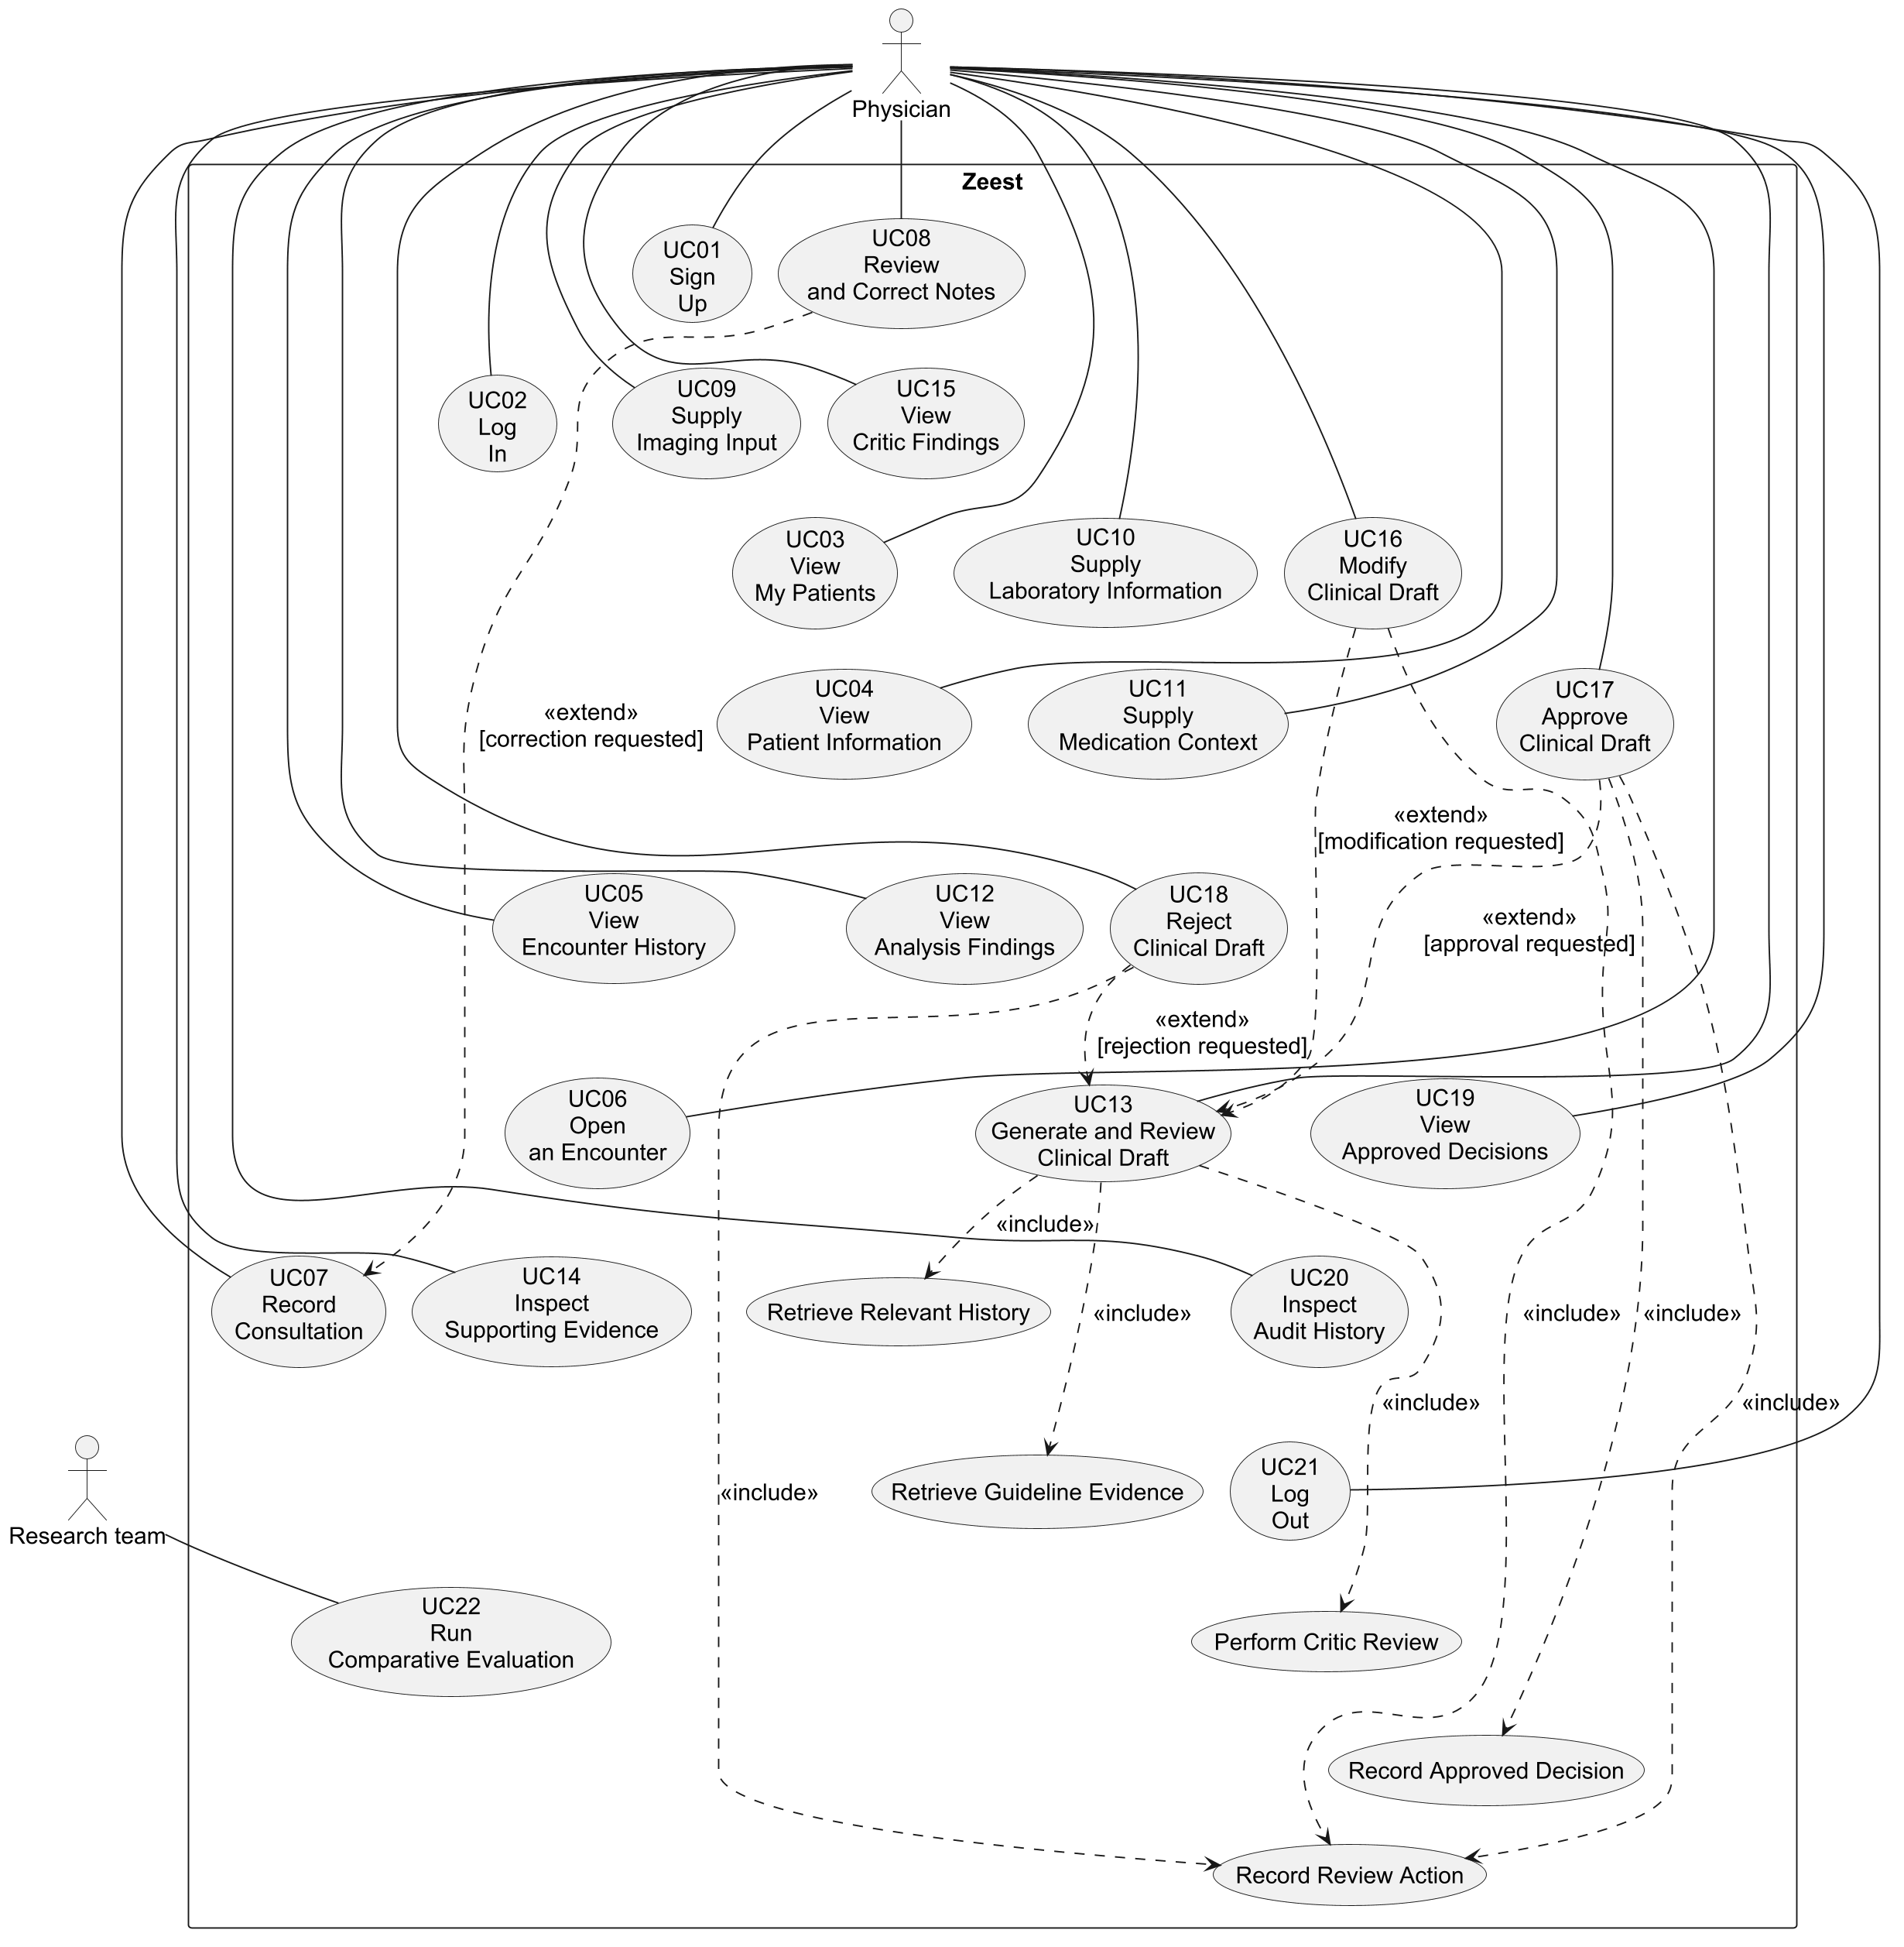
\includegraphics[width=0.96\textwidth,height=0.78\textheight,keepaspectratio]{Figures/kashaf_D01_doctor_use_cases.png}
\caption{Zeest use cases inside one system boundary, with Physician and Research team actors outside. Dashed arrows distinguish mandatory included processing from conditional review actions.}
\label{fig:kashaf:usecases}
\end{figure}

\begin{reporttable}
\centering
\small
\caption{UC01: Sign Up.}
\label{tab:kashaf:uc01}
\begin{tabular}{|p{0.035\textwidth}|p{0.19\textwidth}|p{0.18\textwidth}|p{0.035\textwidth}|p{0.36\textwidth}|}
\hline
\multicolumn{2}{|p{\dimexpr0.225\textwidth+2\tabcolsep+\arrayrulewidth\relax}|}{Name} & \multicolumn{3}{p{\dimexpr0.575\textwidth+4\tabcolsep+2\arrayrulewidth\relax}|}{UC01: Sign Up} \\ \hline
\multicolumn{2}{|p{\dimexpr0.225\textwidth+2\tabcolsep+\arrayrulewidth\relax}|}{Actors} & \multicolumn{3}{p{\dimexpr0.575\textwidth+4\tabcolsep+2\arrayrulewidth\relax}|}{Physician} \\ \hline
\multicolumn{2}{|p{\dimexpr0.225\textwidth+2\tabcolsep+\arrayrulewidth\relax}|}{Summary} & \multicolumn{3}{p{\dimexpr0.575\textwidth+4\tabcolsep+2\arrayrulewidth\relax}|}{The physician creates an account using their registration information.} \\ \hline
\multicolumn{2}{|p{\dimexpr0.225\textwidth+2\tabcolsep+\arrayrulewidth\relax}|}{Pre-Conditions} & \multicolumn{3}{p{\dimexpr0.575\textwidth+4\tabcolsep+2\arrayrulewidth\relax}|}{The physician is not logged in and registration is available.} \\ \hline
\multicolumn{2}{|p{\dimexpr0.225\textwidth+2\tabcolsep+\arrayrulewidth\relax}|}{Post-Conditions} & \multicolumn{3}{p{\dimexpr0.575\textwidth+4\tabcolsep+2\arrayrulewidth\relax}|}{An account is created and the login page is displayed.} \\ \hline
\multicolumn{2}{|p{\dimexpr0.225\textwidth+2\tabcolsep+\arrayrulewidth\relax}|}{Special Requirements} & \multicolumn{3}{p{\dimexpr0.575\textwidth+4\tabcolsep+2\arrayrulewidth\relax}|}{Valid email address; required name and password; securely stored password.} \\ \hline
\multicolumn{5}{|c|}{Basic Flow} \\ \hline
\multicolumn{3}{|c|}{Actor Action} & \multicolumn{2}{c|}{System Response} \\ \hline
1 & \multicolumn{2}{p{\dimexpr0.37\textwidth+2\tabcolsep+\arrayrulewidth\relax}|}{Selects Sign Up.} & 2 & Displays the registration form. \\ \hline
3 & \multicolumn{2}{p{\dimexpr0.37\textwidth+2\tabcolsep+\arrayrulewidth\relax}|}{Enters name, email and password and submits.} & 4 & Validates the information, creates the account and displays Log In. \\ \hline
\multicolumn{5}{|c|}{Alternative Flow} \\ \hline
3 & \multicolumn{2}{p{\dimexpr0.37\textwidth+2\tabcolsep+\arrayrulewidth\relax}|}{Submits incomplete or invalid information.} & 4-A & Identifies the invalid or missing fields without creating an account. \\ \hline
3 & \multicolumn{2}{p{\dimexpr0.37\textwidth+2\tabcolsep+\arrayrulewidth\relax}|}{Uses an email already registered.} & 4-B & Explains that the email is already registered without creating another account. \\ \hline
\end{tabular}
\end{reporttable}

\begin{reporttable}
\centering
\small
\caption{UC02: Log In.}
\label{tab:kashaf:uc02}
\begin{tabular}{|p{0.035\textwidth}|p{0.19\textwidth}|p{0.18\textwidth}|p{0.035\textwidth}|p{0.36\textwidth}|}
\hline
\multicolumn{2}{|p{\dimexpr0.225\textwidth+2\tabcolsep+\arrayrulewidth\relax}|}{Name} & \multicolumn{3}{p{\dimexpr0.575\textwidth+4\tabcolsep+2\arrayrulewidth\relax}|}{UC02: Log In} \\ \hline
\multicolumn{2}{|p{\dimexpr0.225\textwidth+2\tabcolsep+\arrayrulewidth\relax}|}{Actors} & \multicolumn{3}{p{\dimexpr0.575\textwidth+4\tabcolsep+2\arrayrulewidth\relax}|}{Physician} \\ \hline
\multicolumn{2}{|p{\dimexpr0.225\textwidth+2\tabcolsep+\arrayrulewidth\relax}|}{Summary} & \multicolumn{3}{p{\dimexpr0.575\textwidth+4\tabcolsep+2\arrayrulewidth\relax}|}{The physician accesses their account and patient records.} \\ \hline
\multicolumn{2}{|p{\dimexpr0.225\textwidth+2\tabcolsep+\arrayrulewidth\relax}|}{Pre-Conditions} & \multicolumn{3}{p{\dimexpr0.575\textwidth+4\tabcolsep+2\arrayrulewidth\relax}|}{The physician has a registered account and is not logged in.} \\ \hline
\multicolumn{2}{|p{\dimexpr0.225\textwidth+2\tabcolsep+\arrayrulewidth\relax}|}{Post-Conditions} & \multicolumn{3}{p{\dimexpr0.575\textwidth+4\tabcolsep+2\arrayrulewidth\relax}|}{An authenticated session is established.} \\ \hline
\multicolumn{2}{|p{\dimexpr0.225\textwidth+2\tabcolsep+\arrayrulewidth\relax}|}{Special Requirements} & \multicolumn{3}{p{\dimexpr0.575\textwidth+4\tabcolsep+2\arrayrulewidth\relax}|}{Valid registered email and password.} \\ \hline
\multicolumn{5}{|c|}{Basic Flow} \\ \hline
\multicolumn{3}{|c|}{Actor Action} & \multicolumn{2}{c|}{System Response} \\ \hline
1 & \multicolumn{2}{p{\dimexpr0.37\textwidth+2\tabcolsep+\arrayrulewidth\relax}|}{Selects Log In.} & 2 & Displays the login form. \\ \hline
3 & \multicolumn{2}{p{\dimexpr0.37\textwidth+2\tabcolsep+\arrayrulewidth\relax}|}{Enters email and password and submits.} & 4 & Authenticates the account and opens its patient list. \\ \hline
\multicolumn{5}{|c|}{Alternative Flow} \\ \hline
3 & \multicolumn{2}{p{\dimexpr0.37\textwidth+2\tabcolsep+\arrayrulewidth\relax}|}{Enters invalid credentials.} & 4-A & Displays an invalid-credentials message without establishing a session. \\ \hline
\end{tabular}
\end{reporttable}

\begin{reporttable}
\centering
\small
\caption{UC03: View My Patients.}
\label{tab:kashaf:uc03}
\begin{tabular}{|p{0.035\textwidth}|p{0.19\textwidth}|p{0.18\textwidth}|p{0.035\textwidth}|p{0.36\textwidth}|}
\hline
\multicolumn{2}{|p{\dimexpr0.225\textwidth+2\tabcolsep+\arrayrulewidth\relax}|}{Name} & \multicolumn{3}{p{\dimexpr0.575\textwidth+4\tabcolsep+2\arrayrulewidth\relax}|}{UC03: View My Patients} \\ \hline
\multicolumn{2}{|p{\dimexpr0.225\textwidth+2\tabcolsep+\arrayrulewidth\relax}|}{Actors} & \multicolumn{3}{p{\dimexpr0.575\textwidth+4\tabcolsep+2\arrayrulewidth\relax}|}{Physician} \\ \hline
\multicolumn{2}{|p{\dimexpr0.225\textwidth+2\tabcolsep+\arrayrulewidth\relax}|}{Summary} & \multicolumn{3}{p{\dimexpr0.575\textwidth+4\tabcolsep+2\arrayrulewidth\relax}|}{The physician views and selects from their patient records.} \\ \hline
\multicolumn{2}{|p{\dimexpr0.225\textwidth+2\tabcolsep+\arrayrulewidth\relax}|}{Pre-Conditions} & \multicolumn{3}{p{\dimexpr0.575\textwidth+4\tabcolsep+2\arrayrulewidth\relax}|}{The physician is logged in.} \\ \hline
\multicolumn{2}{|p{\dimexpr0.225\textwidth+2\tabcolsep+\arrayrulewidth\relax}|}{Post-Conditions} & \multicolumn{3}{p{\dimexpr0.575\textwidth+4\tabcolsep+2\arrayrulewidth\relax}|}{The physician's patient list is displayed.} \\ \hline
\multicolumn{2}{|p{\dimexpr0.225\textwidth+2\tabcolsep+\arrayrulewidth\relax}|}{Special Requirements} & \multicolumn{3}{p{\dimexpr0.575\textwidth+4\tabcolsep+2\arrayrulewidth\relax}|}{Only records belonging to the logged-in physician are accessible.} \\ \hline
\multicolumn{5}{|c|}{Basic Flow} \\ \hline
\multicolumn{3}{|c|}{Actor Action} & \multicolumn{2}{c|}{System Response} \\ \hline
1 & \multicolumn{2}{p{\dimexpr0.37\textwidth+2\tabcolsep+\arrayrulewidth\relax}|}{Opens My Patients.} & 2 & Retrieves and displays only the physician's patient records. \\ \hline
3 & \multicolumn{2}{p{\dimexpr0.37\textwidth+2\tabcolsep+\arrayrulewidth\relax}|}{Selects a patient.} & 4 & Retains the selected patient and provides access to their information. \\ \hline
\multicolumn{5}{|c|}{Alternative Flow} \\ \hline
1 & \multicolumn{2}{p{\dimexpr0.37\textwidth+2\tabcolsep+\arrayrulewidth\relax}|}{Opens a list without assigned patients.} & 2-A & Displays an empty patient-list message. \\ \hline
\end{tabular}
\end{reporttable}

\begin{reporttable}
\centering
\small
\caption{UC04: View Patient Information.}
\label{tab:kashaf:uc04}
\begin{tabular}{|p{0.035\textwidth}|p{0.19\textwidth}|p{0.18\textwidth}|p{0.035\textwidth}|p{0.36\textwidth}|}
\hline
\multicolumn{2}{|p{\dimexpr0.225\textwidth+2\tabcolsep+\arrayrulewidth\relax}|}{Name} & \multicolumn{3}{p{\dimexpr0.575\textwidth+4\tabcolsep+2\arrayrulewidth\relax}|}{UC04: View Patient Information} \\ \hline
\multicolumn{2}{|p{\dimexpr0.225\textwidth+2\tabcolsep+\arrayrulewidth\relax}|}{Actors} & \multicolumn{3}{p{\dimexpr0.575\textwidth+4\tabcolsep+2\arrayrulewidth\relax}|}{Physician} \\ \hline
\multicolumn{2}{|p{\dimexpr0.225\textwidth+2\tabcolsep+\arrayrulewidth\relax}|}{Summary} & \multicolumn{3}{p{\dimexpr0.575\textwidth+4\tabcolsep+2\arrayrulewidth\relax}|}{The physician reviews the selected patient's available information.} \\ \hline
\multicolumn{2}{|p{\dimexpr0.225\textwidth+2\tabcolsep+\arrayrulewidth\relax}|}{Pre-Conditions} & \multicolumn{3}{p{\dimexpr0.575\textwidth+4\tabcolsep+2\arrayrulewidth\relax}|}{The physician is logged in and one of their own patients is selected.} \\ \hline
\multicolumn{2}{|p{\dimexpr0.225\textwidth+2\tabcolsep+\arrayrulewidth\relax}|}{Post-Conditions} & \multicolumn{3}{p{\dimexpr0.575\textwidth+4\tabcolsep+2\arrayrulewidth\relax}|}{Patient information is displayed.} \\ \hline
\multicolumn{2}{|p{\dimexpr0.225\textwidth+2\tabcolsep+\arrayrulewidth\relax}|}{Special Requirements} & \multicolumn{3}{p{\dimexpr0.575\textwidth+4\tabcolsep+2\arrayrulewidth\relax}|}{Physician ownership must be checked before displaying the record.} \\ \hline
\multicolumn{5}{|c|}{Basic Flow} \\ \hline
\multicolumn{3}{|c|}{Actor Action} & \multicolumn{2}{c|}{System Response} \\ \hline
1 & \multicolumn{2}{p{\dimexpr0.37\textwidth+2\tabcolsep+\arrayrulewidth\relax}|}{Opens the selected patient.} & 2 & Checks ownership and displays patient information. \\ \hline
3 & \multicolumn{2}{p{\dimexpr0.37\textwidth+2\tabcolsep+\arrayrulewidth\relax}|}{Reviews the information.} & 4 & Keeps the selected patient context for subsequent actions. \\ \hline
\multicolumn{5}{|c|}{Alternative Flow} \\ \hline
1 & \multicolumn{2}{p{\dimexpr0.37\textwidth+2\tabcolsep+\arrayrulewidth\relax}|}{Requests another physician's patient record.} & 2-A & Denies access without displaying the record. \\ \hline
\end{tabular}
\end{reporttable}

\begin{reporttable}
\centering
\small
\caption{UC05: View Encounter History.}
\label{tab:kashaf:uc05}
\begin{tabular}{|p{0.035\textwidth}|p{0.19\textwidth}|p{0.18\textwidth}|p{0.035\textwidth}|p{0.36\textwidth}|}
\hline
\multicolumn{2}{|p{\dimexpr0.225\textwidth+2\tabcolsep+\arrayrulewidth\relax}|}{Name} & \multicolumn{3}{p{\dimexpr0.575\textwidth+4\tabcolsep+2\arrayrulewidth\relax}|}{UC05: View Encounter History} \\ \hline
\multicolumn{2}{|p{\dimexpr0.225\textwidth+2\tabcolsep+\arrayrulewidth\relax}|}{Actors} & \multicolumn{3}{p{\dimexpr0.575\textwidth+4\tabcolsep+2\arrayrulewidth\relax}|}{Physician} \\ \hline
\multicolumn{2}{|p{\dimexpr0.225\textwidth+2\tabcolsep+\arrayrulewidth\relax}|}{Summary} & \multicolumn{3}{p{\dimexpr0.575\textwidth+4\tabcolsep+2\arrayrulewidth\relax}|}{The physician reviews the selected patient's previous encounters.} \\ \hline
\multicolumn{2}{|p{\dimexpr0.225\textwidth+2\tabcolsep+\arrayrulewidth\relax}|}{Pre-Conditions} & \multicolumn{3}{p{\dimexpr0.575\textwidth+4\tabcolsep+2\arrayrulewidth\relax}|}{The physician is logged in and one of their own patients is selected.} \\ \hline
\multicolumn{2}{|p{\dimexpr0.225\textwidth+2\tabcolsep+\arrayrulewidth\relax}|}{Post-Conditions} & \multicolumn{3}{p{\dimexpr0.575\textwidth+4\tabcolsep+2\arrayrulewidth\relax}|}{Historical encounter information is displayed.} \\ \hline
\multicolumn{2}{|p{\dimexpr0.225\textwidth+2\tabcolsep+\arrayrulewidth\relax}|}{Special Requirements} & \multicolumn{3}{p{\dimexpr0.575\textwidth+4\tabcolsep+2\arrayrulewidth\relax}|}{History must retain its patient, encounter and source relationships.} \\ \hline
\multicolumn{5}{|c|}{Basic Flow} \\ \hline
\multicolumn{3}{|c|}{Actor Action} & \multicolumn{2}{c|}{System Response} \\ \hline
1 & \multicolumn{2}{p{\dimexpr0.37\textwidth+2\tabcolsep+\arrayrulewidth\relax}|}{Selects Encounter History.} & 2 & Displays the patient's previous encounters. \\ \hline
3 & \multicolumn{2}{p{\dimexpr0.37\textwidth+2\tabcolsep+\arrayrulewidth\relax}|}{Selects a previous encounter.} & 4 & Displays available notes and clinical information with their sources. \\ \hline
\multicolumn{5}{|c|}{Alternative Flow} \\ \hline
1 & \multicolumn{2}{p{\dimexpr0.37\textwidth+2\tabcolsep+\arrayrulewidth\relax}|}{Opens history with no previous encounters.} & 2-A & Displays an empty-history message. \\ \hline
\end{tabular}
\end{reporttable}

\begin{reporttable}
\centering
\small
\caption{UC06: Open an Encounter.}
\label{tab:kashaf:uc06}
\begin{tabular}{|p{0.035\textwidth}|p{0.19\textwidth}|p{0.18\textwidth}|p{0.035\textwidth}|p{0.36\textwidth}|}
\hline
\multicolumn{2}{|p{\dimexpr0.225\textwidth+2\tabcolsep+\arrayrulewidth\relax}|}{Name} & \multicolumn{3}{p{\dimexpr0.575\textwidth+4\tabcolsep+2\arrayrulewidth\relax}|}{UC06: Open an Encounter} \\ \hline
\multicolumn{2}{|p{\dimexpr0.225\textwidth+2\tabcolsep+\arrayrulewidth\relax}|}{Actors} & \multicolumn{3}{p{\dimexpr0.575\textwidth+4\tabcolsep+2\arrayrulewidth\relax}|}{Physician} \\ \hline
\multicolumn{2}{|p{\dimexpr0.225\textwidth+2\tabcolsep+\arrayrulewidth\relax}|}{Summary} & \multicolumn{3}{p{\dimexpr0.575\textwidth+4\tabcolsep+2\arrayrulewidth\relax}|}{The physician opens the encounter used for consultation and review.} \\ \hline
\multicolumn{2}{|p{\dimexpr0.225\textwidth+2\tabcolsep+\arrayrulewidth\relax}|}{Pre-Conditions} & \multicolumn{3}{p{\dimexpr0.575\textwidth+4\tabcolsep+2\arrayrulewidth\relax}|}{The physician is logged in and one of their own patients is selected. An encounter record exists.} \\ \hline
\multicolumn{2}{|p{\dimexpr0.225\textwidth+2\tabcolsep+\arrayrulewidth\relax}|}{Post-Conditions} & \multicolumn{3}{p{\dimexpr0.575\textwidth+4\tabcolsep+2\arrayrulewidth\relax}|}{The encounter becomes the context for clinical actions.} \\ \hline
\multicolumn{2}{|p{\dimexpr0.225\textwidth+2\tabcolsep+\arrayrulewidth\relax}|}{Special Requirements} & \multicolumn{3}{p{\dimexpr0.575\textwidth+4\tabcolsep+2\arrayrulewidth\relax}|}{The encounter must belong to the selected patient and physician.} \\ \hline
\multicolumn{5}{|c|}{Basic Flow} \\ \hline
\multicolumn{3}{|c|}{Actor Action} & \multicolumn{2}{c|}{System Response} \\ \hline
1 & \multicolumn{2}{p{\dimexpr0.37\textwidth+2\tabcolsep+\arrayrulewidth\relax}|}{Selects an encounter.} & 2 & Checks its patient and physician associations. \\ \hline
3 & \multicolumn{2}{p{\dimexpr0.37\textwidth+2\tabcolsep+\arrayrulewidth\relax}|}{Opens the encounter.} & 4 & Displays its consultation workspace and existing inputs. \\ \hline
\multicolumn{5}{|c|}{Alternative Flow} \\ \hline
1 & \multicolumn{2}{p{\dimexpr0.37\textwidth+2\tabcolsep+\arrayrulewidth\relax}|}{Selects an unavailable or unauthorised encounter.} & 2-A & Rejects the selection without exposing its information. \\ \hline
\end{tabular}
\end{reporttable}

\begin{reporttable}
\centering
\small
\caption{UC07: Record Consultation.}
\label{tab:kashaf:uc07}
\begin{tabular}{|p{0.035\textwidth}|p{0.19\textwidth}|p{0.18\textwidth}|p{0.035\textwidth}|p{0.36\textwidth}|}
\hline
\multicolumn{2}{|p{\dimexpr0.225\textwidth+2\tabcolsep+\arrayrulewidth\relax}|}{Name} & \multicolumn{3}{p{\dimexpr0.575\textwidth+4\tabcolsep+2\arrayrulewidth\relax}|}{UC07: Record Consultation} \\ \hline
\multicolumn{2}{|p{\dimexpr0.225\textwidth+2\tabcolsep+\arrayrulewidth\relax}|}{Actors} & \multicolumn{3}{p{\dimexpr0.575\textwidth+4\tabcolsep+2\arrayrulewidth\relax}|}{Physician} \\ \hline
\multicolumn{2}{|p{\dimexpr0.225\textwidth+2\tabcolsep+\arrayrulewidth\relax}|}{Summary} & \multicolumn{3}{p{\dimexpr0.575\textwidth+4\tabcolsep+2\arrayrulewidth\relax}|}{The physician captures audio and obtains structured consultation notes.} \\ \hline
\multicolumn{2}{|p{\dimexpr0.225\textwidth+2\tabcolsep+\arrayrulewidth\relax}|}{Pre-Conditions} & \multicolumn{3}{p{\dimexpr0.575\textwidth+4\tabcolsep+2\arrayrulewidth\relax}|}{The physician is logged in and an encounter for one of their own patients is open.} \\ \hline
\multicolumn{2}{|p{\dimexpr0.225\textwidth+2\tabcolsep+\arrayrulewidth\relax}|}{Post-Conditions} & \multicolumn{3}{p{\dimexpr0.575\textwidth+4\tabcolsep+2\arrayrulewidth\relax}|}{Captured consultation content is presented as structured notes.} \\ \hline
\multicolumn{2}{|p{\dimexpr0.225\textwidth+2\tabcolsep+\arrayrulewidth\relax}|}{Special Requirements} & \multicolumn{3}{p{\dimexpr0.575\textwidth+4\tabcolsep+2\arrayrulewidth\relax}|}{Working microphone, recording permission and supported transcription service.} \\ \hline
\multicolumn{5}{|c|}{Basic Flow} \\ \hline
\multicolumn{3}{|c|}{Actor Action} & \multicolumn{2}{c|}{System Response} \\ \hline
1 & \multicolumn{2}{p{\dimexpr0.37\textwidth+2\tabcolsep+\arrayrulewidth\relax}|}{Selects Start Recording.} & 2 & Checks audio access and begins capture and transcription. \\ \hline
3 & \multicolumn{2}{p{\dimexpr0.37\textwidth+2\tabcolsep+\arrayrulewidth\relax}|}{Conducts the consultation.} & 4 & Transcribes incoming audio into structured notes. \\ \hline
5 & \multicolumn{2}{p{\dimexpr0.37\textwidth+2\tabcolsep+\arrayrulewidth\relax}|}{Selects Stop Recording.} & 6 & Stops capture and presents the resulting notes. \\ \hline
\multicolumn{5}{|c|}{Alternative Flow} \\ \hline
1 & \multicolumn{2}{p{\dimexpr0.37\textwidth+2\tabcolsep+\arrayrulewidth\relax}|}{Cannot grant microphone permission.} & 2-A & Reports the access problem without recording. \\ \hline
3 & \multicolumn{2}{p{\dimexpr0.37\textwidth+2\tabcolsep+\arrayrulewidth\relax}|}{Continues when transcription fails.} & 4-A & Reports the failure and identifies incomplete notes. \\ \hline
\end{tabular}
\end{reporttable}

\begin{reporttable}
\centering
\small
\caption{UC08: Review and Correct Notes.}
\label{tab:kashaf:uc08}
\begin{tabular}{|p{0.035\textwidth}|p{0.19\textwidth}|p{0.18\textwidth}|p{0.035\textwidth}|p{0.36\textwidth}|}
\hline
\multicolumn{2}{|p{\dimexpr0.225\textwidth+2\tabcolsep+\arrayrulewidth\relax}|}{Name} & \multicolumn{3}{p{\dimexpr0.575\textwidth+4\tabcolsep+2\arrayrulewidth\relax}|}{UC08: Review and Correct Notes} \\ \hline
\multicolumn{2}{|p{\dimexpr0.225\textwidth+2\tabcolsep+\arrayrulewidth\relax}|}{Actors} & \multicolumn{3}{p{\dimexpr0.575\textwidth+4\tabcolsep+2\arrayrulewidth\relax}|}{Physician} \\ \hline
\multicolumn{2}{|p{\dimexpr0.225\textwidth+2\tabcolsep+\arrayrulewidth\relax}|}{Summary} & \multicolumn{3}{p{\dimexpr0.575\textwidth+4\tabcolsep+2\arrayrulewidth\relax}|}{The physician reviews and saves corrections to consultation notes.} \\ \hline
\multicolumn{2}{|p{\dimexpr0.225\textwidth+2\tabcolsep+\arrayrulewidth\relax}|}{Pre-Conditions} & \multicolumn{3}{p{\dimexpr0.575\textwidth+4\tabcolsep+2\arrayrulewidth\relax}|}{The physician is logged in and an encounter for one of their own patients is open. Structured notes are available.} \\ \hline
\multicolumn{2}{|p{\dimexpr0.225\textwidth+2\tabcolsep+\arrayrulewidth\relax}|}{Post-Conditions} & \multicolumn{3}{p{\dimexpr0.575\textwidth+4\tabcolsep+2\arrayrulewidth\relax}|}{The reviewed notes are retained for the encounter.} \\ \hline
\multicolumn{2}{|p{\dimexpr0.225\textwidth+2\tabcolsep+\arrayrulewidth\relax}|}{Special Requirements} & \multicolumn{3}{p{\dimexpr0.575\textwidth+4\tabcolsep+2\arrayrulewidth\relax}|}{Corrections must preserve the encounter association.} \\ \hline
\multicolumn{5}{|c|}{Basic Flow} \\ \hline
\multicolumn{3}{|c|}{Actor Action} & \multicolumn{2}{c|}{System Response} \\ \hline
1 & \multicolumn{2}{p{\dimexpr0.37\textwidth+2\tabcolsep+\arrayrulewidth\relax}|}{Opens the notes.} & 2 & Displays the available structured notes. \\ \hline
3 & \multicolumn{2}{p{\dimexpr0.37\textwidth+2\tabcolsep+\arrayrulewidth\relax}|}{Edits the notes and selects Save.} & 4 & Validates and saves the corrected content. \\ \hline
\multicolumn{5}{|c|}{Alternative Flow} \\ \hline
3 & \multicolumn{2}{p{\dimexpr0.37\textwidth+2\tabcolsep+\arrayrulewidth\relax}|}{Submits unusable note content.} & 4-A & Requests correction and retains the prior saved content. \\ \hline
\end{tabular}
\end{reporttable}

\begin{reporttable}
\centering
\small
\caption{UC09: Supply Imaging Input.}
\label{tab:kashaf:uc09}
\begin{tabular}{|p{0.035\textwidth}|p{0.19\textwidth}|p{0.18\textwidth}|p{0.035\textwidth}|p{0.36\textwidth}|}
\hline
\multicolumn{2}{|p{\dimexpr0.225\textwidth+2\tabcolsep+\arrayrulewidth\relax}|}{Name} & \multicolumn{3}{p{\dimexpr0.575\textwidth+4\tabcolsep+2\arrayrulewidth\relax}|}{UC09: Supply Imaging Input} \\ \hline
\multicolumn{2}{|p{\dimexpr0.225\textwidth+2\tabcolsep+\arrayrulewidth\relax}|}{Actors} & \multicolumn{3}{p{\dimexpr0.575\textwidth+4\tabcolsep+2\arrayrulewidth\relax}|}{Physician} \\ \hline
\multicolumn{2}{|p{\dimexpr0.225\textwidth+2\tabcolsep+\arrayrulewidth\relax}|}{Summary} & \multicolumn{3}{p{\dimexpr0.575\textwidth+4\tabcolsep+2\arrayrulewidth\relax}|}{The physician supplies imaging information for the selected encounter.} \\ \hline
\multicolumn{2}{|p{\dimexpr0.225\textwidth+2\tabcolsep+\arrayrulewidth\relax}|}{Pre-Conditions} & \multicolumn{3}{p{\dimexpr0.575\textwidth+4\tabcolsep+2\arrayrulewidth\relax}|}{The physician is logged in and an encounter for one of their own patients is open.} \\ \hline
\multicolumn{2}{|p{\dimexpr0.225\textwidth+2\tabcolsep+\arrayrulewidth\relax}|}{Post-Conditions} & \multicolumn{3}{p{\dimexpr0.575\textwidth+4\tabcolsep+2\arrayrulewidth\relax}|}{The supplied input is retained and submitted to its specialist agent.} \\ \hline
\multicolumn{2}{|p{\dimexpr0.225\textwidth+2\tabcolsep+\arrayrulewidth\relax}|}{Special Requirements} & \multicolumn{3}{p{\dimexpr0.575\textwidth+4\tabcolsep+2\arrayrulewidth\relax}|}{Input must meet the selected imaging model's supported format and task.} \\ \hline
\multicolumn{5}{|c|}{Basic Flow} \\ \hline
\multicolumn{3}{|c|}{Actor Action} & \multicolumn{2}{c|}{System Response} \\ \hline
1 & \multicolumn{2}{p{\dimexpr0.37\textwidth+2\tabcolsep+\arrayrulewidth\relax}|}{Opens the imaging input control.} & 2 & Displays the supported input requirements. \\ \hline
3 & \multicolumn{2}{p{\dimexpr0.37\textwidth+2\tabcolsep+\arrayrulewidth\relax}|}{Provides the input and submits.} & 4 & Validates the input and submits it for specialised processing. \\ \hline
\multicolumn{5}{|c|}{Alternative Flow} \\ \hline
3 & \multicolumn{2}{p{\dimexpr0.37\textwidth+2\tabcolsep+\arrayrulewidth\relax}|}{Submits missing or unsupported input.} & 4-A & Explains the validation problem without treating the input as processed. \\ \hline
\end{tabular}
\end{reporttable}

\begin{reporttable}
\centering
\small
\caption{UC10: Supply Laboratory Information.}
\label{tab:kashaf:uc10}
\begin{tabular}{|p{0.035\textwidth}|p{0.19\textwidth}|p{0.18\textwidth}|p{0.035\textwidth}|p{0.36\textwidth}|}
\hline
\multicolumn{2}{|p{\dimexpr0.225\textwidth+2\tabcolsep+\arrayrulewidth\relax}|}{Name} & \multicolumn{3}{p{\dimexpr0.575\textwidth+4\tabcolsep+2\arrayrulewidth\relax}|}{UC10: Supply Laboratory Information} \\ \hline
\multicolumn{2}{|p{\dimexpr0.225\textwidth+2\tabcolsep+\arrayrulewidth\relax}|}{Actors} & \multicolumn{3}{p{\dimexpr0.575\textwidth+4\tabcolsep+2\arrayrulewidth\relax}|}{Physician} \\ \hline
\multicolumn{2}{|p{\dimexpr0.225\textwidth+2\tabcolsep+\arrayrulewidth\relax}|}{Summary} & \multicolumn{3}{p{\dimexpr0.575\textwidth+4\tabcolsep+2\arrayrulewidth\relax}|}{The physician supplies laboratory information for the selected encounter.} \\ \hline
\multicolumn{2}{|p{\dimexpr0.225\textwidth+2\tabcolsep+\arrayrulewidth\relax}|}{Pre-Conditions} & \multicolumn{3}{p{\dimexpr0.575\textwidth+4\tabcolsep+2\arrayrulewidth\relax}|}{The physician is logged in and an encounter for one of their own patients is open.} \\ \hline
\multicolumn{2}{|p{\dimexpr0.225\textwidth+2\tabcolsep+\arrayrulewidth\relax}|}{Post-Conditions} & \multicolumn{3}{p{\dimexpr0.575\textwidth+4\tabcolsep+2\arrayrulewidth\relax}|}{The supplied input is retained and submitted to its specialist agent.} \\ \hline
\multicolumn{2}{|p{\dimexpr0.225\textwidth+2\tabcolsep+\arrayrulewidth\relax}|}{Special Requirements} & \multicolumn{3}{p{\dimexpr0.575\textwidth+4\tabcolsep+2\arrayrulewidth\relax}|}{Laboratory values must retain their supplied units and source context.} \\ \hline
\multicolumn{5}{|c|}{Basic Flow} \\ \hline
\multicolumn{3}{|c|}{Actor Action} & \multicolumn{2}{c|}{System Response} \\ \hline
1 & \multicolumn{2}{p{\dimexpr0.37\textwidth+2\tabcolsep+\arrayrulewidth\relax}|}{Opens the laboratory input control.} & 2 & Displays the supported input requirements. \\ \hline
3 & \multicolumn{2}{p{\dimexpr0.37\textwidth+2\tabcolsep+\arrayrulewidth\relax}|}{Provides the input and submits.} & 4 & Validates the input and submits it for specialised processing. \\ \hline
\multicolumn{5}{|c|}{Alternative Flow} \\ \hline
3 & \multicolumn{2}{p{\dimexpr0.37\textwidth+2\tabcolsep+\arrayrulewidth\relax}|}{Submits missing or unsupported input.} & 4-A & Explains the validation problem without treating the input as processed. \\ \hline
\end{tabular}
\end{reporttable}

\begin{reporttable}
\centering
\small
\caption{UC11: Supply Medication Context.}
\label{tab:kashaf:uc11}
\begin{tabular}{|p{0.035\textwidth}|p{0.19\textwidth}|p{0.18\textwidth}|p{0.035\textwidth}|p{0.36\textwidth}|}
\hline
\multicolumn{2}{|p{\dimexpr0.225\textwidth+2\tabcolsep+\arrayrulewidth\relax}|}{Name} & \multicolumn{3}{p{\dimexpr0.575\textwidth+4\tabcolsep+2\arrayrulewidth\relax}|}{UC11: Supply Medication Context} \\ \hline
\multicolumn{2}{|p{\dimexpr0.225\textwidth+2\tabcolsep+\arrayrulewidth\relax}|}{Actors} & \multicolumn{3}{p{\dimexpr0.575\textwidth+4\tabcolsep+2\arrayrulewidth\relax}|}{Physician} \\ \hline
\multicolumn{2}{|p{\dimexpr0.225\textwidth+2\tabcolsep+\arrayrulewidth\relax}|}{Summary} & \multicolumn{3}{p{\dimexpr0.575\textwidth+4\tabcolsep+2\arrayrulewidth\relax}|}{The physician supplies medication information for the selected encounter.} \\ \hline
\multicolumn{2}{|p{\dimexpr0.225\textwidth+2\tabcolsep+\arrayrulewidth\relax}|}{Pre-Conditions} & \multicolumn{3}{p{\dimexpr0.575\textwidth+4\tabcolsep+2\arrayrulewidth\relax}|}{The physician is logged in and an encounter for one of their own patients is open.} \\ \hline
\multicolumn{2}{|p{\dimexpr0.225\textwidth+2\tabcolsep+\arrayrulewidth\relax}|}{Post-Conditions} & \multicolumn{3}{p{\dimexpr0.575\textwidth+4\tabcolsep+2\arrayrulewidth\relax}|}{The supplied input is retained and submitted to its specialist agent.} \\ \hline
\multicolumn{2}{|p{\dimexpr0.225\textwidth+2\tabcolsep+\arrayrulewidth\relax}|}{Special Requirements} & \multicolumn{3}{p{\dimexpr0.575\textwidth+4\tabcolsep+2\arrayrulewidth\relax}|}{Medication information must remain linked to the selected patient and encounter.} \\ \hline
\multicolumn{5}{|c|}{Basic Flow} \\ \hline
\multicolumn{3}{|c|}{Actor Action} & \multicolumn{2}{c|}{System Response} \\ \hline
1 & \multicolumn{2}{p{\dimexpr0.37\textwidth+2\tabcolsep+\arrayrulewidth\relax}|}{Opens the medication input control.} & 2 & Displays the supported input requirements. \\ \hline
3 & \multicolumn{2}{p{\dimexpr0.37\textwidth+2\tabcolsep+\arrayrulewidth\relax}|}{Provides the input and submits.} & 4 & Validates the input and submits it for specialised processing. \\ \hline
\multicolumn{5}{|c|}{Alternative Flow} \\ \hline
3 & \multicolumn{2}{p{\dimexpr0.37\textwidth+2\tabcolsep+\arrayrulewidth\relax}|}{Submits missing or unsupported input.} & 4-A & Explains the validation problem without treating the input as processed. \\ \hline
\end{tabular}
\end{reporttable}

\begin{reporttable}
\centering
\small
\caption{UC12: View Analysis Findings.}
\label{tab:kashaf:uc12}
\begin{tabular}{|p{0.035\textwidth}|p{0.19\textwidth}|p{0.18\textwidth}|p{0.035\textwidth}|p{0.36\textwidth}|}
\hline
\multicolumn{2}{|p{\dimexpr0.225\textwidth+2\tabcolsep+\arrayrulewidth\relax}|}{Name} & \multicolumn{3}{p{\dimexpr0.575\textwidth+4\tabcolsep+2\arrayrulewidth\relax}|}{UC12: View Analysis Findings} \\ \hline
\multicolumn{2}{|p{\dimexpr0.225\textwidth+2\tabcolsep+\arrayrulewidth\relax}|}{Actors} & \multicolumn{3}{p{\dimexpr0.575\textwidth+4\tabcolsep+2\arrayrulewidth\relax}|}{Physician} \\ \hline
\multicolumn{2}{|p{\dimexpr0.225\textwidth+2\tabcolsep+\arrayrulewidth\relax}|}{Summary} & \multicolumn{3}{p{\dimexpr0.575\textwidth+4\tabcolsep+2\arrayrulewidth\relax}|}{The physician inspects specialist findings for the encounter.} \\ \hline
\multicolumn{2}{|p{\dimexpr0.225\textwidth+2\tabcolsep+\arrayrulewidth\relax}|}{Pre-Conditions} & \multicolumn{3}{p{\dimexpr0.575\textwidth+4\tabcolsep+2\arrayrulewidth\relax}|}{The physician is logged in and an encounter for one of their own patients is open. Clinical inputs have been submitted.} \\ \hline
\multicolumn{2}{|p{\dimexpr0.225\textwidth+2\tabcolsep+\arrayrulewidth\relax}|}{Post-Conditions} & \multicolumn{3}{p{\dimexpr0.575\textwidth+4\tabcolsep+2\arrayrulewidth\relax}|}{Available findings and processing states are displayed.} \\ \hline
\multicolumn{2}{|p{\dimexpr0.225\textwidth+2\tabcolsep+\arrayrulewidth\relax}|}{Special Requirements} & \multicolumn{3}{p{\dimexpr0.575\textwidth+4\tabcolsep+2\arrayrulewidth\relax}|}{Findings must identify their source; failures must not appear as successful results.} \\ \hline
\multicolumn{5}{|c|}{Basic Flow} \\ \hline
\multicolumn{3}{|c|}{Actor Action} & \multicolumn{2}{c|}{System Response} \\ \hline
1 & \multicolumn{2}{p{\dimexpr0.37\textwidth+2\tabcolsep+\arrayrulewidth\relax}|}{Opens Analysis Findings.} & 2 & Displays imaging, laboratory and medication results with processing states. \\ \hline
3 & \multicolumn{2}{p{\dimexpr0.37\textwidth+2\tabcolsep+\arrayrulewidth\relax}|}{Selects a finding.} & 4 & Displays its source and available analysis information. \\ \hline
\multicolumn{5}{|c|}{Alternative Flow} \\ \hline
1 & \multicolumn{2}{p{\dimexpr0.37\textwidth+2\tabcolsep+\arrayrulewidth\relax}|}{Requests findings while processing is incomplete.} & 2-A & Displays the pending or failed state rather than a completed result. \\ \hline
\end{tabular}
\end{reporttable}

\begin{reporttable}
\centering
\small
\caption{UC13: Generate and Review Clinical Draft.}
\label{tab:kashaf:uc13}
\begin{tabular}{|p{0.035\textwidth}|p{0.19\textwidth}|p{0.18\textwidth}|p{0.035\textwidth}|p{0.36\textwidth}|}
\hline
\multicolumn{2}{|p{\dimexpr0.225\textwidth+2\tabcolsep+\arrayrulewidth\relax}|}{Name} & \multicolumn{3}{p{\dimexpr0.575\textwidth+4\tabcolsep+2\arrayrulewidth\relax}|}{UC13: Generate and Review Clinical Draft} \\ \hline
\multicolumn{2}{|p{\dimexpr0.225\textwidth+2\tabcolsep+\arrayrulewidth\relax}|}{Actors} & \multicolumn{3}{p{\dimexpr0.575\textwidth+4\tabcolsep+2\arrayrulewidth\relax}|}{Physician} \\ \hline
\multicolumn{2}{|p{\dimexpr0.225\textwidth+2\tabcolsep+\arrayrulewidth\relax}|}{Summary} & \multicolumn{3}{p{\dimexpr0.575\textwidth+4\tabcolsep+2\arrayrulewidth\relax}|}{The physician requests a diagnosis and treatment draft for review.} \\ \hline
\multicolumn{2}{|p{\dimexpr0.225\textwidth+2\tabcolsep+\arrayrulewidth\relax}|}{Pre-Conditions} & \multicolumn{3}{p{\dimexpr0.575\textwidth+4\tabcolsep+2\arrayrulewidth\relax}|}{The physician is logged in and an encounter for one of their own patients is open. Case information is available.} \\ \hline
\multicolumn{2}{|p{\dimexpr0.225\textwidth+2\tabcolsep+\arrayrulewidth\relax}|}{Post-Conditions} & \multicolumn{3}{p{\dimexpr0.575\textwidth+4\tabcolsep+2\arrayrulewidth\relax}|}{An evidence-supported draft and critic findings are available for physician review.} \\ \hline
\multicolumn{2}{|p{\dimexpr0.225\textwidth+2\tabcolsep+\arrayrulewidth\relax}|}{Special Requirements} & \multicolumn{3}{p{\dimexpr0.575\textwidth+4\tabcolsep+2\arrayrulewidth\relax}|}{Relevant history, evidence retrieval and critic review precede presentation.} \\ \hline
\multicolumn{5}{|c|}{Basic Flow} \\ \hline
\multicolumn{3}{|c|}{Actor Action} & \multicolumn{2}{c|}{System Response} \\ \hline
1 & \multicolumn{2}{p{\dimexpr0.37\textwidth+2\tabcolsep+\arrayrulewidth\relax}|}{Selects Generate Draft.} & 2 & Prepares the case with inputs, specialist findings and relevant history. \\ \hline
3 & \multicolumn{2}{p{\dimexpr0.37\textwidth+2\tabcolsep+\arrayrulewidth\relax}|}{Waits for the requested draft.} & 4 & Retrieves evidence, generates the draft, performs critic review and presents the output. \\ \hline
5 & \multicolumn{2}{p{\dimexpr0.37\textwidth+2\tabcolsep+\arrayrulewidth\relax}|}{Reviews the presented draft, evidence and critic findings.} & 6 & Keeps the draft pending while the physician chooses a review action. \\ \hline
\multicolumn{5}{|c|}{Alternative Flow} \\ \hline
1 & \multicolumn{2}{p{\dimexpr0.37\textwidth+2\tabcolsep+\arrayrulewidth\relax}|}{Requests generation without usable case information.} & 2-A & Explains the missing inputs. \\ \hline
3 & \multicolumn{2}{p{\dimexpr0.37\textwidth+2\tabcolsep+\arrayrulewidth\relax}|}{Waits during a processing failure.} & 4-A & Reports the failed stage without presenting an unreviewed output as completed. \\ \hline
\end{tabular}
\end{reporttable}

\begin{reporttable}
\centering
\small
\caption{UC14: Inspect Supporting Evidence.}
\label{tab:kashaf:uc14}
\begin{tabular}{|p{0.035\textwidth}|p{0.19\textwidth}|p{0.18\textwidth}|p{0.035\textwidth}|p{0.36\textwidth}|}
\hline
\multicolumn{2}{|p{\dimexpr0.225\textwidth+2\tabcolsep+\arrayrulewidth\relax}|}{Name} & \multicolumn{3}{p{\dimexpr0.575\textwidth+4\tabcolsep+2\arrayrulewidth\relax}|}{UC14: Inspect Supporting Evidence} \\ \hline
\multicolumn{2}{|p{\dimexpr0.225\textwidth+2\tabcolsep+\arrayrulewidth\relax}|}{Actors} & \multicolumn{3}{p{\dimexpr0.575\textwidth+4\tabcolsep+2\arrayrulewidth\relax}|}{Physician} \\ \hline
\multicolumn{2}{|p{\dimexpr0.225\textwidth+2\tabcolsep+\arrayrulewidth\relax}|}{Summary} & \multicolumn{3}{p{\dimexpr0.575\textwidth+4\tabcolsep+2\arrayrulewidth\relax}|}{The physician reviews citations and passages supporting the draft.} \\ \hline
\multicolumn{2}{|p{\dimexpr0.225\textwidth+2\tabcolsep+\arrayrulewidth\relax}|}{Pre-Conditions} & \multicolumn{3}{p{\dimexpr0.575\textwidth+4\tabcolsep+2\arrayrulewidth\relax}|}{The physician is logged in and an encounter for one of their own patients is open. A generated draft is available.} \\ \hline
\multicolumn{2}{|p{\dimexpr0.225\textwidth+2\tabcolsep+\arrayrulewidth\relax}|}{Post-Conditions} & \multicolumn{3}{p{\dimexpr0.575\textwidth+4\tabcolsep+2\arrayrulewidth\relax}|}{Available supporting evidence is displayed.} \\ \hline
\multicolumn{2}{|p{\dimexpr0.225\textwidth+2\tabcolsep+\arrayrulewidth\relax}|}{Special Requirements} & \multicolumn{3}{p{\dimexpr0.575\textwidth+4\tabcolsep+2\arrayrulewidth\relax}|}{Citations and passages must retain their source and draft relationships.} \\ \hline
\multicolumn{5}{|c|}{Basic Flow} \\ \hline
\multicolumn{3}{|c|}{Actor Action} & \multicolumn{2}{c|}{System Response} \\ \hline
1 & \multicolumn{2}{p{\dimexpr0.37\textwidth+2\tabcolsep+\arrayrulewidth\relax}|}{Opens Supporting Evidence.} & 2 & Displays citations and retrieved passages. \\ \hline
3 & \multicolumn{2}{p{\dimexpr0.37\textwidth+2\tabcolsep+\arrayrulewidth\relax}|}{Selects an evidence item.} & 4 & Displays its source reference and supporting content. \\ \hline
\multicolumn{5}{|c|}{Alternative Flow} \\ \hline
1 & \multicolumn{2}{p{\dimexpr0.37\textwidth+2\tabcolsep+\arrayrulewidth\relax}|}{Reviews a draft with missing supporting evidence.} & 2-A & Identifies the missing support without inventing citations. \\ \hline
\end{tabular}
\end{reporttable}

\begin{reporttable}
\centering
\small
\caption{UC15: View Critic Findings.}
\label{tab:kashaf:uc15}
\begin{tabular}{|p{0.035\textwidth}|p{0.19\textwidth}|p{0.18\textwidth}|p{0.035\textwidth}|p{0.36\textwidth}|}
\hline
\multicolumn{2}{|p{\dimexpr0.225\textwidth+2\tabcolsep+\arrayrulewidth\relax}|}{Name} & \multicolumn{3}{p{\dimexpr0.575\textwidth+4\tabcolsep+2\arrayrulewidth\relax}|}{UC15: View Critic Findings} \\ \hline
\multicolumn{2}{|p{\dimexpr0.225\textwidth+2\tabcolsep+\arrayrulewidth\relax}|}{Actors} & \multicolumn{3}{p{\dimexpr0.575\textwidth+4\tabcolsep+2\arrayrulewidth\relax}|}{Physician} \\ \hline
\multicolumn{2}{|p{\dimexpr0.225\textwidth+2\tabcolsep+\arrayrulewidth\relax}|}{Summary} & \multicolumn{3}{p{\dimexpr0.575\textwidth+4\tabcolsep+2\arrayrulewidth\relax}|}{The physician reviews the safety and consistency assessment of the draft.} \\ \hline
\multicolumn{2}{|p{\dimexpr0.225\textwidth+2\tabcolsep+\arrayrulewidth\relax}|}{Pre-Conditions} & \multicolumn{3}{p{\dimexpr0.575\textwidth+4\tabcolsep+2\arrayrulewidth\relax}|}{The physician is logged in and an encounter for one of their own patients is open. A generated draft is available. Critic review has been performed.} \\ \hline
\multicolumn{2}{|p{\dimexpr0.225\textwidth+2\tabcolsep+\arrayrulewidth\relax}|}{Post-Conditions} & \multicolumn{3}{p{\dimexpr0.575\textwidth+4\tabcolsep+2\arrayrulewidth\relax}|}{Critic findings are displayed alongside the draft.} \\ \hline
\multicolumn{2}{|p{\dimexpr0.225\textwidth+2\tabcolsep+\arrayrulewidth\relax}|}{Special Requirements} & \multicolumn{3}{p{\dimexpr0.575\textwidth+4\tabcolsep+2\arrayrulewidth\relax}|}{The review must identify the draft it assessed and retain physician decision authority.} \\ \hline
\multicolumn{5}{|c|}{Basic Flow} \\ \hline
\multicolumn{3}{|c|}{Actor Action} & \multicolumn{2}{c|}{System Response} \\ \hline
1 & \multicolumn{2}{p{\dimexpr0.37\textwidth+2\tabcolsep+\arrayrulewidth\relax}|}{Opens Critic Findings.} & 2 & Displays the available safety and consistency findings. \\ \hline
3 & \multicolumn{2}{p{\dimexpr0.37\textwidth+2\tabcolsep+\arrayrulewidth\relax}|}{Reviews a finding.} & 4 & Keeps the finding associated with its assessed draft. \\ \hline
\multicolumn{5}{|c|}{Alternative Flow} \\ \hline
1 & \multicolumn{2}{p{\dimexpr0.37\textwidth+2\tabcolsep+\arrayrulewidth\relax}|}{Requests an unavailable critic review.} & 2-A & Displays its unavailable state without claiming a successful review. \\ \hline
\end{tabular}
\end{reporttable}

\begin{reporttable}
\centering
\small
\caption{UC16: Modify Clinical Draft.}
\label{tab:kashaf:uc16}
\begin{tabular}{|p{0.035\textwidth}|p{0.19\textwidth}|p{0.18\textwidth}|p{0.035\textwidth}|p{0.36\textwidth}|}
\hline
\multicolumn{2}{|p{\dimexpr0.225\textwidth+2\tabcolsep+\arrayrulewidth\relax}|}{Name} & \multicolumn{3}{p{\dimexpr0.575\textwidth+4\tabcolsep+2\arrayrulewidth\relax}|}{UC16: Modify Clinical Draft} \\ \hline
\multicolumn{2}{|p{\dimexpr0.225\textwidth+2\tabcolsep+\arrayrulewidth\relax}|}{Actors} & \multicolumn{3}{p{\dimexpr0.575\textwidth+4\tabcolsep+2\arrayrulewidth\relax}|}{Physician} \\ \hline
\multicolumn{2}{|p{\dimexpr0.225\textwidth+2\tabcolsep+\arrayrulewidth\relax}|}{Summary} & \multicolumn{3}{p{\dimexpr0.575\textwidth+4\tabcolsep+2\arrayrulewidth\relax}|}{The physician edits and saves a generated clinical draft.} \\ \hline
\multicolumn{2}{|p{\dimexpr0.225\textwidth+2\tabcolsep+\arrayrulewidth\relax}|}{Pre-Conditions} & \multicolumn{3}{p{\dimexpr0.575\textwidth+4\tabcolsep+2\arrayrulewidth\relax}|}{The physician is logged in and an encounter for one of their own patients is open. A generated draft is available. The draft is pending review.} \\ \hline
\multicolumn{2}{|p{\dimexpr0.225\textwidth+2\tabcolsep+\arrayrulewidth\relax}|}{Post-Conditions} & \multicolumn{3}{p{\dimexpr0.575\textwidth+4\tabcolsep+2\arrayrulewidth\relax}|}{A revised draft is saved and remains pending approval.} \\ \hline
\multicolumn{2}{|p{\dimexpr0.225\textwidth+2\tabcolsep+\arrayrulewidth\relax}|}{Special Requirements} & \multicolumn{3}{p{\dimexpr0.575\textwidth+4\tabcolsep+2\arrayrulewidth\relax}|}{Saving a modification must not record an approved decision.} \\ \hline
\multicolumn{5}{|c|}{Basic Flow} \\ \hline
\multicolumn{3}{|c|}{Actor Action} & \multicolumn{2}{c|}{System Response} \\ \hline
1 & \multicolumn{2}{p{\dimexpr0.37\textwidth+2\tabcolsep+\arrayrulewidth\relax}|}{Selects Modify.} & 2 & Displays editable draft content. \\ \hline
3 & \multicolumn{2}{p{\dimexpr0.37\textwidth+2\tabcolsep+\arrayrulewidth\relax}|}{Edits the content and selects Save.} & 4 & Stores the revised draft and modification action without approval. \\ \hline
\multicolumn{5}{|c|}{Alternative Flow} \\ \hline
3 & \multicolumn{2}{p{\dimexpr0.37\textwidth+2\tabcolsep+\arrayrulewidth\relax}|}{Cancels the edit.} & 4-A & Retains the previous saved revision. \\ \hline
\end{tabular}
\end{reporttable}

\begin{reporttable}
\centering
\small
\caption{UC17: Approve Clinical Draft.}
\label{tab:kashaf:uc17}
\begin{tabular}{|p{0.035\textwidth}|p{0.19\textwidth}|p{0.18\textwidth}|p{0.035\textwidth}|p{0.36\textwidth}|}
\hline
\multicolumn{2}{|p{\dimexpr0.225\textwidth+2\tabcolsep+\arrayrulewidth\relax}|}{Name} & \multicolumn{3}{p{\dimexpr0.575\textwidth+4\tabcolsep+2\arrayrulewidth\relax}|}{UC17: Approve Clinical Draft} \\ \hline
\multicolumn{2}{|p{\dimexpr0.225\textwidth+2\tabcolsep+\arrayrulewidth\relax}|}{Actors} & \multicolumn{3}{p{\dimexpr0.575\textwidth+4\tabcolsep+2\arrayrulewidth\relax}|}{Physician} \\ \hline
\multicolumn{2}{|p{\dimexpr0.225\textwidth+2\tabcolsep+\arrayrulewidth\relax}|}{Summary} & \multicolumn{3}{p{\dimexpr0.575\textwidth+4\tabcolsep+2\arrayrulewidth\relax}|}{The physician explicitly accepts the reviewed draft revision.} \\ \hline
\multicolumn{2}{|p{\dimexpr0.225\textwidth+2\tabcolsep+\arrayrulewidth\relax}|}{Pre-Conditions} & \multicolumn{3}{p{\dimexpr0.575\textwidth+4\tabcolsep+2\arrayrulewidth\relax}|}{The physician is logged in and an encounter for one of their own patients is open. A generated draft is available. The displayed revision is pending review.} \\ \hline
\multicolumn{2}{|p{\dimexpr0.225\textwidth+2\tabcolsep+\arrayrulewidth\relax}|}{Post-Conditions} & \multicolumn{3}{p{\dimexpr0.575\textwidth+4\tabcolsep+2\arrayrulewidth\relax}|}{The accepted content is recorded as an approved clinical decision.} \\ \hline
\multicolumn{2}{|p{\dimexpr0.225\textwidth+2\tabcolsep+\arrayrulewidth\relax}|}{Special Requirements} & \multicolumn{3}{p{\dimexpr0.575\textwidth+4\tabcolsep+2\arrayrulewidth\relax}|}{Approval must identify the exact saved revision and responsible physician.} \\ \hline
\multicolumn{5}{|c|}{Basic Flow} \\ \hline
\multicolumn{3}{|c|}{Actor Action} & \multicolumn{2}{c|}{System Response} \\ \hline
1 & \multicolumn{2}{p{\dimexpr0.37\textwidth+2\tabcolsep+\arrayrulewidth\relax}|}{Selects Approve.} & 2 & Displays the revision and content to confirm. \\ \hline
3 & \multicolumn{2}{p{\dimexpr0.37\textwidth+2\tabcolsep+\arrayrulewidth\relax}|}{Confirms approval.} & 4 & Records the accepted decision and corresponding audit action. \\ \hline
\multicolumn{5}{|c|}{Alternative Flow} \\ \hline
3 & \multicolumn{2}{p{\dimexpr0.37\textwidth+2\tabcolsep+\arrayrulewidth\relax}|}{Confirms after the revision has changed.} & 4-A & Requests review of the current saved revision before approval. \\ \hline
3 & \multicolumn{2}{p{\dimexpr0.37\textwidth+2\tabcolsep+\arrayrulewidth\relax}|}{Cancels confirmation.} & 4-B & Leaves the draft pending. \\ \hline
\end{tabular}
\end{reporttable}

\begin{reporttable}
\centering
\small
\caption{UC18: Reject Clinical Draft.}
\label{tab:kashaf:uc18}
\begin{tabular}{|p{0.035\textwidth}|p{0.19\textwidth}|p{0.18\textwidth}|p{0.035\textwidth}|p{0.36\textwidth}|}
\hline
\multicolumn{2}{|p{\dimexpr0.225\textwidth+2\tabcolsep+\arrayrulewidth\relax}|}{Name} & \multicolumn{3}{p{\dimexpr0.575\textwidth+4\tabcolsep+2\arrayrulewidth\relax}|}{UC18: Reject Clinical Draft} \\ \hline
\multicolumn{2}{|p{\dimexpr0.225\textwidth+2\tabcolsep+\arrayrulewidth\relax}|}{Actors} & \multicolumn{3}{p{\dimexpr0.575\textwidth+4\tabcolsep+2\arrayrulewidth\relax}|}{Physician} \\ \hline
\multicolumn{2}{|p{\dimexpr0.225\textwidth+2\tabcolsep+\arrayrulewidth\relax}|}{Summary} & \multicolumn{3}{p{\dimexpr0.575\textwidth+4\tabcolsep+2\arrayrulewidth\relax}|}{The physician rejects a pending clinical draft.} \\ \hline
\multicolumn{2}{|p{\dimexpr0.225\textwidth+2\tabcolsep+\arrayrulewidth\relax}|}{Pre-Conditions} & \multicolumn{3}{p{\dimexpr0.575\textwidth+4\tabcolsep+2\arrayrulewidth\relax}|}{The physician is logged in and an encounter for one of their own patients is open. A generated draft is available. The draft is pending review.} \\ \hline
\multicolumn{2}{|p{\dimexpr0.225\textwidth+2\tabcolsep+\arrayrulewidth\relax}|}{Post-Conditions} & \multicolumn{3}{p{\dimexpr0.575\textwidth+4\tabcolsep+2\arrayrulewidth\relax}|}{The draft is marked rejected and the action is logged.} \\ \hline
\multicolumn{2}{|p{\dimexpr0.225\textwidth+2\tabcolsep+\arrayrulewidth\relax}|}{Special Requirements} & \multicolumn{3}{p{\dimexpr0.575\textwidth+4\tabcolsep+2\arrayrulewidth\relax}|}{Rejected content must not become an approved decision.} \\ \hline
\multicolumn{5}{|c|}{Basic Flow} \\ \hline
\multicolumn{3}{|c|}{Actor Action} & \multicolumn{2}{c|}{System Response} \\ \hline
1 & \multicolumn{2}{p{\dimexpr0.37\textwidth+2\tabcolsep+\arrayrulewidth\relax}|}{Selects Reject.} & 2 & Requests confirmation for the selected draft. \\ \hline
3 & \multicolumn{2}{p{\dimexpr0.37\textwidth+2\tabcolsep+\arrayrulewidth\relax}|}{Confirms rejection.} & 4 & Records rejection and its audit action without recording a clinical decision. \\ \hline
\multicolumn{5}{|c|}{Alternative Flow} \\ \hline
3 & \multicolumn{2}{p{\dimexpr0.37\textwidth+2\tabcolsep+\arrayrulewidth\relax}|}{Cancels rejection.} & 4-A & Leaves the existing draft state unchanged. \\ \hline
\end{tabular}
\end{reporttable}

\begin{reporttable}
\centering
\small
\caption{UC19: View Approved Decisions.}
\label{tab:kashaf:uc19}
\begin{tabular}{|p{0.035\textwidth}|p{0.19\textwidth}|p{0.18\textwidth}|p{0.035\textwidth}|p{0.36\textwidth}|}
\hline
\multicolumn{2}{|p{\dimexpr0.225\textwidth+2\tabcolsep+\arrayrulewidth\relax}|}{Name} & \multicolumn{3}{p{\dimexpr0.575\textwidth+4\tabcolsep+2\arrayrulewidth\relax}|}{UC19: View Approved Decisions} \\ \hline
\multicolumn{2}{|p{\dimexpr0.225\textwidth+2\tabcolsep+\arrayrulewidth\relax}|}{Actors} & \multicolumn{3}{p{\dimexpr0.575\textwidth+4\tabcolsep+2\arrayrulewidth\relax}|}{Physician} \\ \hline
\multicolumn{2}{|p{\dimexpr0.225\textwidth+2\tabcolsep+\arrayrulewidth\relax}|}{Summary} & \multicolumn{3}{p{\dimexpr0.575\textwidth+4\tabcolsep+2\arrayrulewidth\relax}|}{The physician reviews accepted decisions for their selected patient.} \\ \hline
\multicolumn{2}{|p{\dimexpr0.225\textwidth+2\tabcolsep+\arrayrulewidth\relax}|}{Pre-Conditions} & \multicolumn{3}{p{\dimexpr0.575\textwidth+4\tabcolsep+2\arrayrulewidth\relax}|}{The physician is logged in and one of their own patients is selected.} \\ \hline
\multicolumn{2}{|p{\dimexpr0.225\textwidth+2\tabcolsep+\arrayrulewidth\relax}|}{Post-Conditions} & \multicolumn{3}{p{\dimexpr0.575\textwidth+4\tabcolsep+2\arrayrulewidth\relax}|}{Approved decision content and its encounter context are displayed.} \\ \hline
\multicolumn{2}{|p{\dimexpr0.225\textwidth+2\tabcolsep+\arrayrulewidth\relax}|}{Special Requirements} & \multicolumn{3}{p{\dimexpr0.575\textwidth+4\tabcolsep+2\arrayrulewidth\relax}|}{Only explicitly approved decisions belonging to the physician's patient may be displayed.} \\ \hline
\multicolumn{5}{|c|}{Basic Flow} \\ \hline
\multicolumn{3}{|c|}{Actor Action} & \multicolumn{2}{c|}{System Response} \\ \hline
1 & \multicolumn{2}{p{\dimexpr0.37\textwidth+2\tabcolsep+\arrayrulewidth\relax}|}{Opens Approved Decisions.} & 2 & Displays the patient's approved decisions grouped by encounter. \\ \hline
3 & \multicolumn{2}{p{\dimexpr0.37\textwidth+2\tabcolsep+\arrayrulewidth\relax}|}{Selects a decision.} & 4 & Displays accepted content and its approval context. \\ \hline
\multicolumn{5}{|c|}{Alternative Flow} \\ \hline
1 & \multicolumn{2}{p{\dimexpr0.37\textwidth+2\tabcolsep+\arrayrulewidth\relax}|}{Opens a patient with no approved decisions.} & 2-A & Displays an empty approved-decisions message. \\ \hline
\end{tabular}
\end{reporttable}

\begin{reporttable}
\centering
\small
\caption{UC20: Inspect Audit History.}
\label{tab:kashaf:uc20}
\begin{tabular}{|p{0.035\textwidth}|p{0.19\textwidth}|p{0.18\textwidth}|p{0.035\textwidth}|p{0.36\textwidth}|}
\hline
\multicolumn{2}{|p{\dimexpr0.225\textwidth+2\tabcolsep+\arrayrulewidth\relax}|}{Name} & \multicolumn{3}{p{\dimexpr0.575\textwidth+4\tabcolsep+2\arrayrulewidth\relax}|}{UC20: Inspect Audit History} \\ \hline
\multicolumn{2}{|p{\dimexpr0.225\textwidth+2\tabcolsep+\arrayrulewidth\relax}|}{Actors} & \multicolumn{3}{p{\dimexpr0.575\textwidth+4\tabcolsep+2\arrayrulewidth\relax}|}{Physician} \\ \hline
\multicolumn{2}{|p{\dimexpr0.225\textwidth+2\tabcolsep+\arrayrulewidth\relax}|}{Summary} & \multicolumn{3}{p{\dimexpr0.575\textwidth+4\tabcolsep+2\arrayrulewidth\relax}|}{The physician reviews the encounter's recorded decision actions.} \\ \hline
\multicolumn{2}{|p{\dimexpr0.225\textwidth+2\tabcolsep+\arrayrulewidth\relax}|}{Pre-Conditions} & \multicolumn{3}{p{\dimexpr0.575\textwidth+4\tabcolsep+2\arrayrulewidth\relax}|}{The physician is logged in and an encounter for one of their own patients is open.} \\ \hline
\multicolumn{2}{|p{\dimexpr0.225\textwidth+2\tabcolsep+\arrayrulewidth\relax}|}{Post-Conditions} & \multicolumn{3}{p{\dimexpr0.575\textwidth+4\tabcolsep+2\arrayrulewidth\relax}|}{Review actions are displayed without changing them.} \\ \hline
\multicolumn{2}{|p{\dimexpr0.225\textwidth+2\tabcolsep+\arrayrulewidth\relax}|}{Special Requirements} & \multicolumn{3}{p{\dimexpr0.575\textwidth+4\tabcolsep+2\arrayrulewidth\relax}|}{Actions must retain time, physician identity, draft revision and encounter context.} \\ \hline
\multicolumn{5}{|c|}{Basic Flow} \\ \hline
\multicolumn{3}{|c|}{Actor Action} & \multicolumn{2}{c|}{System Response} \\ \hline
1 & \multicolumn{2}{p{\dimexpr0.37\textwidth+2\tabcolsep+\arrayrulewidth\relax}|}{Opens Audit History.} & 2 & Displays recorded review actions. \\ \hline
3 & \multicolumn{2}{p{\dimexpr0.37\textwidth+2\tabcolsep+\arrayrulewidth\relax}|}{Selects an action.} & 4 & Displays its revision and decision context. \\ \hline
\multicolumn{5}{|c|}{Alternative Flow} \\ \hline
1 & \multicolumn{2}{p{\dimexpr0.37\textwidth+2\tabcolsep+\arrayrulewidth\relax}|}{Opens an encounter without review actions.} & 2-A & Displays an empty audit-history message. \\ \hline
\end{tabular}
\end{reporttable}

\begin{reporttable}
\centering
\small
\caption{UC21: Log Out.}
\label{tab:kashaf:uc21}
\begin{tabular}{|p{0.035\textwidth}|p{0.19\textwidth}|p{0.18\textwidth}|p{0.035\textwidth}|p{0.36\textwidth}|}
\hline
\multicolumn{2}{|p{\dimexpr0.225\textwidth+2\tabcolsep+\arrayrulewidth\relax}|}{Name} & \multicolumn{3}{p{\dimexpr0.575\textwidth+4\tabcolsep+2\arrayrulewidth\relax}|}{UC21: Log Out} \\ \hline
\multicolumn{2}{|p{\dimexpr0.225\textwidth+2\tabcolsep+\arrayrulewidth\relax}|}{Actors} & \multicolumn{3}{p{\dimexpr0.575\textwidth+4\tabcolsep+2\arrayrulewidth\relax}|}{Physician} \\ \hline
\multicolumn{2}{|p{\dimexpr0.225\textwidth+2\tabcolsep+\arrayrulewidth\relax}|}{Summary} & \multicolumn{3}{p{\dimexpr0.575\textwidth+4\tabcolsep+2\arrayrulewidth\relax}|}{The physician ends the application session.} \\ \hline
\multicolumn{2}{|p{\dimexpr0.225\textwidth+2\tabcolsep+\arrayrulewidth\relax}|}{Pre-Conditions} & \multicolumn{3}{p{\dimexpr0.575\textwidth+4\tabcolsep+2\arrayrulewidth\relax}|}{The physician is logged in.} \\ \hline
\multicolumn{2}{|p{\dimexpr0.225\textwidth+2\tabcolsep+\arrayrulewidth\relax}|}{Post-Conditions} & \multicolumn{3}{p{\dimexpr0.575\textwidth+4\tabcolsep+2\arrayrulewidth\relax}|}{The session ends and protected records require login.} \\ \hline
\multicolumn{2}{|p{\dimexpr0.225\textwidth+2\tabcolsep+\arrayrulewidth\relax}|}{Special Requirements} & \multicolumn{3}{p{\dimexpr0.575\textwidth+4\tabcolsep+2\arrayrulewidth\relax}|}{Protected patient information must not remain accessible through the ended session.} \\ \hline
\multicolumn{5}{|c|}{Basic Flow} \\ \hline
\multicolumn{3}{|c|}{Actor Action} & \multicolumn{2}{c|}{System Response} \\ \hline
1 & \multicolumn{2}{p{\dimexpr0.37\textwidth+2\tabcolsep+\arrayrulewidth\relax}|}{Selects Log Out.} & 2 & Terminates the session and displays Log In. \\ \hline
\multicolumn{5}{|c|}{Alternative Flow} \\ \hline
1 & \multicolumn{2}{p{\dimexpr0.37\textwidth+2\tabcolsep+\arrayrulewidth\relax}|}{Selects Log Out after the session has expired.} & 2-A & Displays Log In without restoring access. \\ \hline
\end{tabular}
\end{reporttable}

\begin{reporttable}
\centering
\small
\caption{UC22: Run Comparative Evaluation.}
\label{tab:kashaf:uc22}
\begin{tabular}{|p{0.035\textwidth}|p{0.19\textwidth}|p{0.18\textwidth}|p{0.035\textwidth}|p{0.36\textwidth}|}
\hline
\multicolumn{2}{|p{\dimexpr0.225\textwidth+2\tabcolsep+\arrayrulewidth\relax}|}{Name} & \multicolumn{3}{p{\dimexpr0.575\textwidth+4\tabcolsep+2\arrayrulewidth\relax}|}{UC22: Run Comparative Evaluation} \\ \hline
\multicolumn{2}{|p{\dimexpr0.225\textwidth+2\tabcolsep+\arrayrulewidth\relax}|}{Actors} & \multicolumn{3}{p{\dimexpr0.575\textwidth+4\tabcolsep+2\arrayrulewidth\relax}|}{Research team} \\ \hline
\multicolumn{2}{|p{\dimexpr0.225\textwidth+2\tabcolsep+\arrayrulewidth\relax}|}{Summary} & \multicolumn{3}{p{\dimexpr0.575\textwidth+4\tabcolsep+2\arrayrulewidth\relax}|}{The research team compares the defined system variants.} \\ \hline
\multicolumn{2}{|p{\dimexpr0.225\textwidth+2\tabcolsep+\arrayrulewidth\relax}|}{Pre-Conditions} & \multicolumn{3}{p{\dimexpr0.575\textwidth+4\tabcolsep+2\arrayrulewidth\relax}|}{Permitted cases, reference assessments and configurations are available.} \\ \hline
\multicolumn{2}{|p{\dimexpr0.225\textwidth+2\tabcolsep+\arrayrulewidth\relax}|}{Post-Conditions} & \multicolumn{3}{p{\dimexpr0.575\textwidth+4\tabcolsep+2\arrayrulewidth\relax}|}{Outputs are recorded with their cases and configurations for comparison.} \\ \hline
\multicolumn{2}{|p{\dimexpr0.225\textwidth+2\tabcolsep+\arrayrulewidth\relax}|}{Special Requirements} & \multicolumn{3}{p{\dimexpr0.575\textwidth+4\tabcolsep+2\arrayrulewidth\relax}|}{The baseline, memory variant and full system must use consistent assessment conditions.} \\ \hline
\multicolumn{5}{|c|}{Basic Flow} \\ \hline
\multicolumn{3}{|c|}{Actor Action} & \multicolumn{2}{c|}{System Response} \\ \hline
1 & \multicolumn{2}{p{\dimexpr0.37\textwidth+2\tabcolsep+\arrayrulewidth\relax}|}{Selects cases and configurations.} & 2 & Checks the required inputs and comparison settings. \\ \hline
3 & \multicolumn{2}{p{\dimexpr0.37\textwidth+2\tabcolsep+\arrayrulewidth\relax}|}{Starts evaluation.} & 4 & Runs the variants and records outputs and configuration details. \\ \hline
\multicolumn{5}{|c|}{Alternative Flow} \\ \hline
1 & \multicolumn{2}{p{\dimexpr0.37\textwidth+2\tabcolsep+\arrayrulewidth\relax}|}{Selects unavailable cases or incomplete settings.} & 2-A & Identifies missing prerequisites without fabricating results. \\ \hline
\end{tabular}
\end{reporttable}


\section{Hardware and Software Requirements}

Tables~\ref{tab:kashaf:hardware} and~\ref{tab:kashaf:software} identify the supporting resources.

\subsection{Hardware Requirements}

A development computer must support the application services, storage and the tools used to integrate the processing components. The physician interface needs a browser-capable device and an audio input source for consultation capture. Microphone access must be available when the recording workflow is used, and connectivity must support whichever processing services are selected. Storage must retain the permitted case inputs, relational records and associated semantic representations without separating them from their identifying context. Compute and memory requirements depend on the imaging and transcription models, the language-model access arrangement and the size of the case collection. Table~\ref{tab:kashaf:hardware} records these resource needs with the configuration values that remain to be established. Numerical compute, storage and concurrent-user limits must be established for the selected workload rather than assumed from a candidate model. Resource failures should be identifiable during integration checks. No resource specification alone establishes measured capacity for the integrated clinical processing workflow.

\begin{reporttable}
\centering
\small
\caption{Hardware resources supporting the Zeest workflow.}
\label{tab:kashaf:hardware}
\begin{tabular}{|p{0.24\textwidth}|p{0.36\textwidth}|p{0.28\textwidth}|}
\hline
Resource & Purpose & Specification \\ \hline
Development/processing computer & Application services and selected local processing & Processor and RAM: TBD after model selection. \\ \hline
Physician device & Web interface and review actions & Browser-capable device; supported configurations: TBD. \\ \hline
Audio input & Consultation capture & Working audio source and capture permission. \\ \hline
Storage & Clinical inputs, records, audit actions and vectors & Capacity and retention configuration: TBD. \\ \hline
Graphics acceleration & Local inference where required & GPU requirement depends on the selected model. \\ \hline
Connectivity & Access to selected processing and evidence services & Connection requirements depend on service arrangement. \\ \hline
\end{tabular}
\end{reporttable}

% Finish this section's floats before the next heading.

\subsection{Software Requirements}

FastAPI provides the backend integration layer, while Next.js supports the physician-facing web interface. LangGraph and Google ADK are the named orchestration technologies for coordinating the agent responsibilities, with their exact division to be agreed in the detailed design. Gemini supplies the language-model capability used within the reasoning workflow, and PyTorch supports integration of the imaging model. PostgreSQL stores patient, encounter and review information, with pgvector providing the semantic representation layer alongside relational records. A transcription component and clinical knowledge resources the dependencies needed for consultation capture, guideline retrieval and medication review. Table~\ref{tab:kashaf:software} connects these technologies to their responsibilities. Component versions, model identifiers, representations and access conditions must be recorded when the environment is selected. Component versions and permitted resource use must be recorded before comparative runs. Framework choices do not establish completed integration or guaranteed compatibility. Each selected dependency requires a recorded configuration and an identifiable integration failure path.

\begin{reporttable}
\centering
\small
\caption{Software technologies and processing dependencies used in the Zeest design.}
\label{tab:kashaf:software}
\begin{tabular}{|p{0.25\textwidth}|p{0.34\textwidth}|p{0.29\textwidth}|}
\hline
Technology/resource & Responsibility & Configuration \\ \hline
FastAPI & Backend integration and application interfaces & Version and interface contracts: TBD. \\ \hline
Next.js & Physician-facing web application & Version: TBD. \\ \hline
LangGraph; Google ADK & Agent orchestration & Responsibility division: TBD. \\ \hline
Gemini & Language-model reasoning & Model and access configuration: TBD. \\ \hline
PyTorch; existing imaging model & Supported image classification & Validated model and label set: TBD. \\ \hline
PostgreSQL; pgvector & Relational records and semantic memory & Embedding model, dimension and versions: TBD. \\ \hline
Transcription component & Audio-to-notes processing & Model, languages and input formats: TBD. \\ \hline
Guidelines; medication knowledge resource & Evidence retrieval and medication review & Selected resources and use conditions: TBD. \\ \hline
MIMIC-IV; MIMIC-CXR; PubMed; Synthea; imaging candidates & Clinical/evidence data and synthetic case strategy & Permitted access and final cases/domain: TBD. \\ \hline
\end{tabular}
\end{reporttable}

% Finish this section's floats before the next heading.

\section{Graphical User Interface}

The physician screens support registration, access to the physician's own patients, encounter review, consultation capture and clinical decisions. Related functions share pages or tabs rather than requiring a separate page for every use case. The research team uses a separate comparative-evaluation screen. Tables~\ref{tab:kashaf:view-map} and~\ref{tab:kashaf:view-review-map} identify each screen, user and covered use case. Figures~\ref{fig:kashaf:navigation}, \ref{fig:kashaf:swimlane-navigation} and~\ref{fig:kashaf:research-navigation} show their navigation. Existing accounts begin at Login; registration is available for new accounts. Review branches to modification, approval or rejection, while accepted decisions and audit actions remain distinguishable. Patient and encounter context is maintained throughout clinical work. Screen captions identify the intended user and covered functionality. These images are interface mockups rather than evidence of executed authentication, recording, analysis or decisions. Empty states and illustrative references show layout only. The primary screen flow and the physician-system swimlane provide complementary views, while the research flow separates evaluation work from clinical review. Implementation testing remains future work.

\begin{reporttable}
\centering
\small
\caption{Physician access, patient and input screens mapped to users and use cases.}
\label{tab:kashaf:view-map}
\begin{tabular}{|p{0.07\textwidth}|p{0.43\textwidth}|p{0.14\textwidth}|p{0.23\textwidth}|}
\hline
Screen & Page / state & User & Use cases \\ \hline
G01 & Sign Up (Figure~\ref{fig:kashaf:gui-signup}) & Physician & UC01 \\ \hline
G02 & Log In (Figure~\ref{fig:kashaf:gui-login}) & Physician & UC02, UC21 \\ \hline
G03 & My Patients (Figure~\ref{fig:kashaf:gui-patients}) & Physician & UC03, UC21 \\ \hline
G04 & Patient Details (Figure~\ref{fig:kashaf:gui-history}) & Physician & UC04--UC06 \\ \hline
G05 & Consultation (Figure~\ref{fig:kashaf:gui-consultation}) & Physician & UC07--UC08 \\ \hline
G06 & Imaging Input and Findings (Figure~\ref{fig:kashaf:gui-imaging}) & Physician & UC09, UC12--UC13 \\ \hline
G07 & Laboratory Input and Findings (Figure~\ref{fig:kashaf:gui-laboratory}) & Physician & UC10, UC12--UC13 \\ \hline
G08 & Medication Input and Findings (Figure~\ref{fig:kashaf:gui-medication}) & Physician & UC11, UC12--UC13 \\ \hline
\end{tabular}
\end{reporttable}

\begin{reporttable}
\centering
\small
\caption{Review, decision, audit and research screens mapped to users and use cases.}
\label{tab:kashaf:view-review-map}
\begin{tabular}{|p{0.07\textwidth}|p{0.43\textwidth}|p{0.14\textwidth}|p{0.23\textwidth}|}
\hline
Screen & Page / state & User & Use cases \\ \hline
G09 & Clinical Review and Evidence (Figure~\ref{fig:kashaf:gui-review}) & Physician & UC13--UC14 \\ \hline
G10 & Critic Findings (Figure~\ref{fig:kashaf:gui-critic}) & Physician & UC15 \\ \hline
G11 & Modify Clinical Draft (Figure~\ref{fig:kashaf:gui-modify}) & Physician & UC16 \\ \hline
G12 & Approval Confirmation (Figure~\ref{fig:kashaf:gui-approve}) & Physician & UC17 \\ \hline
G13 & Rejection Confirmation (Figure~\ref{fig:kashaf:gui-reject}) & Physician & UC18 \\ \hline
G14 & Approved Decisions (Figure~\ref{fig:kashaf:gui-decisions}) & Physician & UC19 \\ \hline
G15 & Audit History (Figure~\ref{fig:kashaf:gui-audit}) & Physician & UC20 \\ \hline
G16 & Comparative Evaluation (Figure~\ref{fig:kashaf:gui-evaluation}) & Research team & UC22 \\ \hline
\end{tabular}
\end{reporttable}


\begin{figure}[!htbp]
\centering
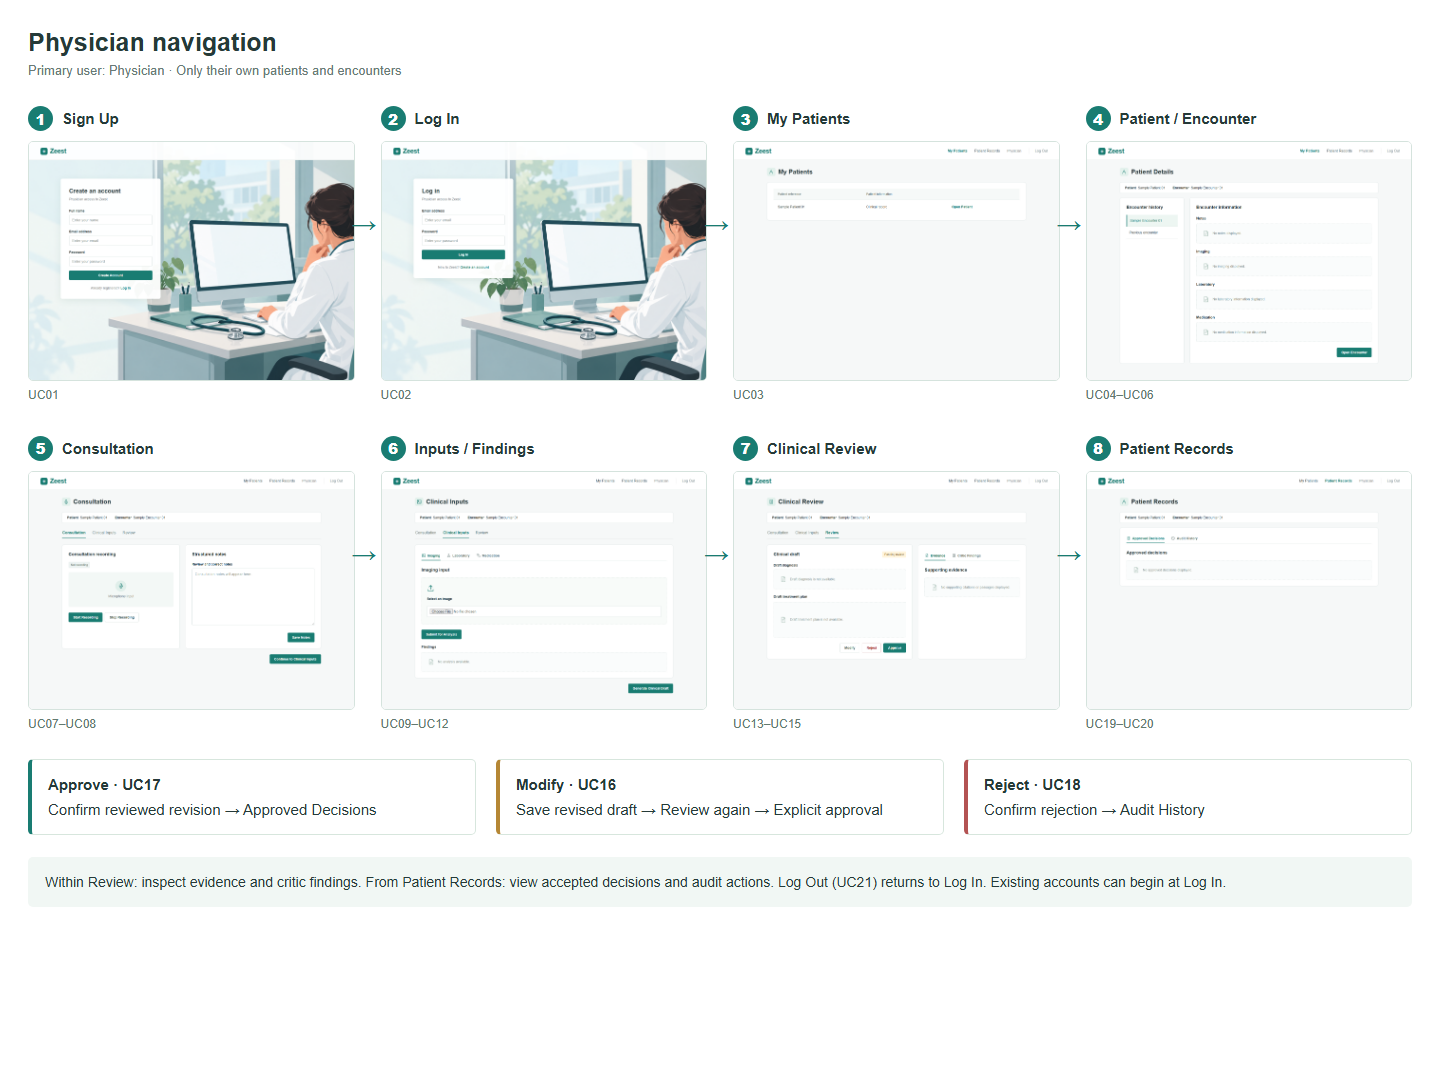
\includegraphics[width=\textwidth,height=0.80\textheight,keepaspectratio]{Figures/kashaf_D02_primary_navigation.png}
\caption{Primary physician navigation through the numbered screen thumbnails. Review branches to modification, approval or rejection; Patient Records exposes approved decisions and audit history. Logout returns to Login.}
\label{fig:kashaf:navigation}
\end{figure}

\begin{figure}[!htbp]
\centering
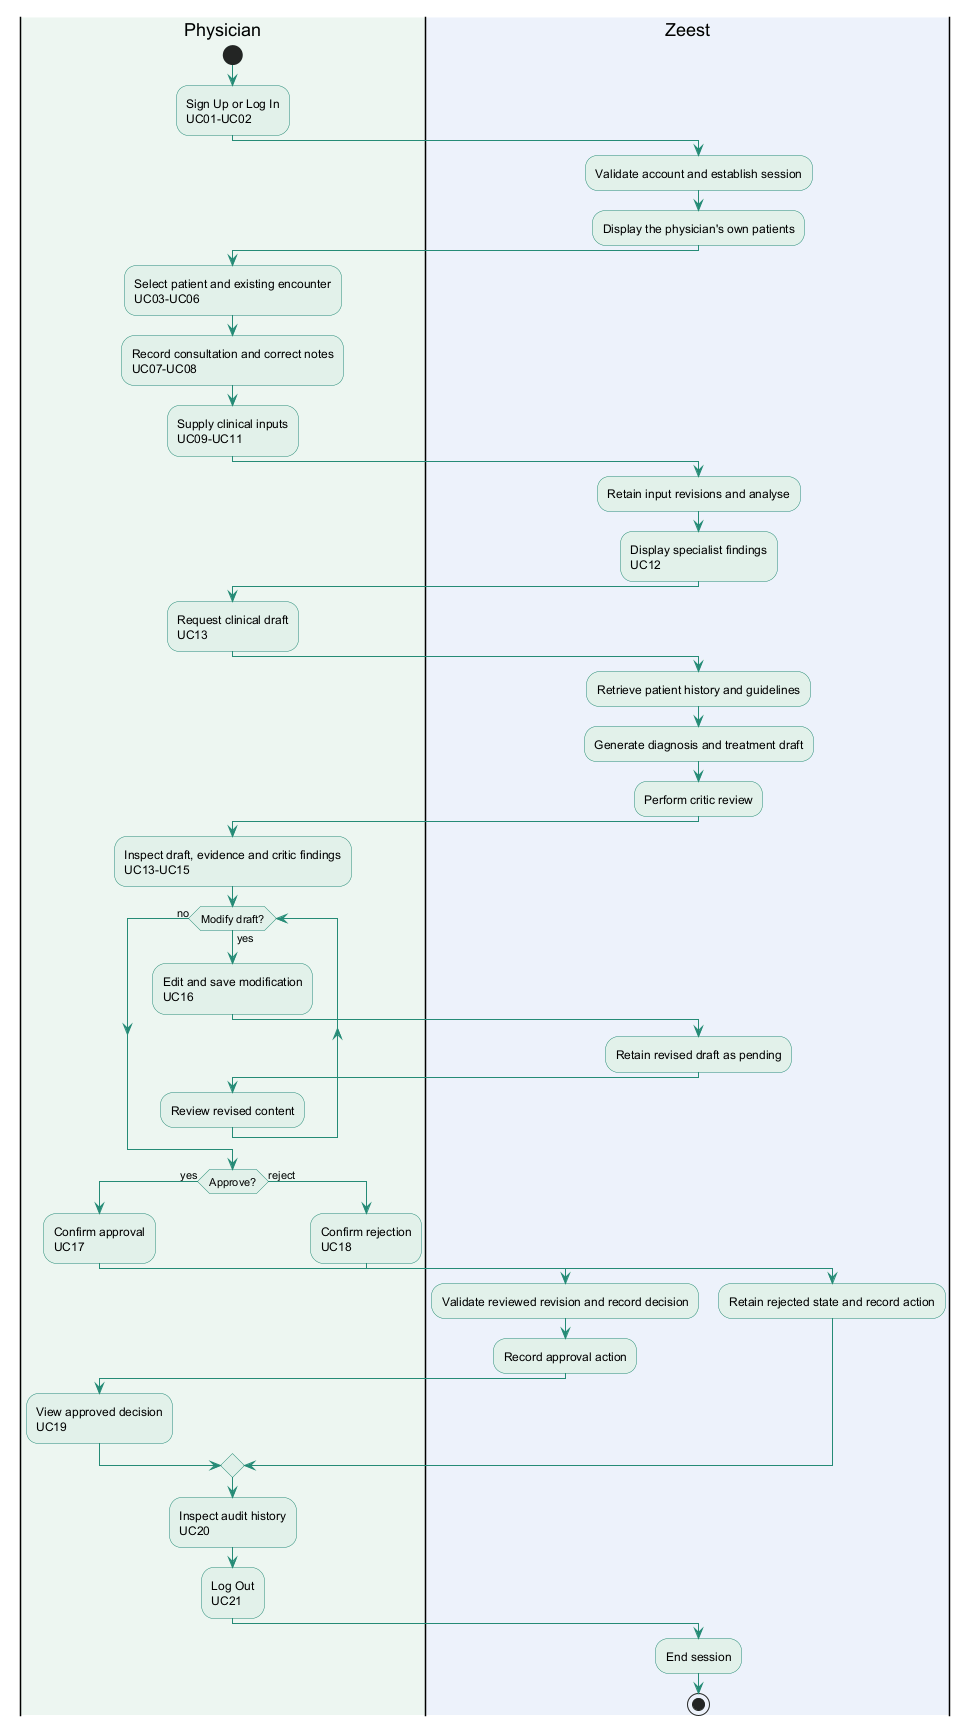
\includegraphics[width=0.96\textwidth,height=0.86\textheight,keepaspectratio]{Figures/kashaf_D02_doctor_navigation.png}
\caption{Physician--Zeest swimlane navigation retained alongside the screen-thumbnail flow. Physician actions appear in the left lane and system processing in the right, including ownership checks, clinical analysis, draft modification, explicit approval or rejection, audit review and logout.}
\label{fig:kashaf:swimlane-navigation}
\end{figure}

\begin{figure}[!htbp]
\centering
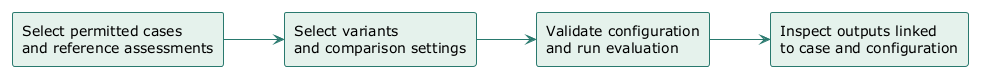
\includegraphics[width=0.96\textwidth,height=.22\textheight,keepaspectratio]{Figures/kashaf_research_navigation.png}
\caption{Research-team navigation for UC22: select permitted cases, configure variants, validate and run evaluation, then inspect outputs associated with each case and configuration.}
\label{fig:kashaf:research-navigation}
\end{figure}

\begin{figure}[!htbp]
\centering
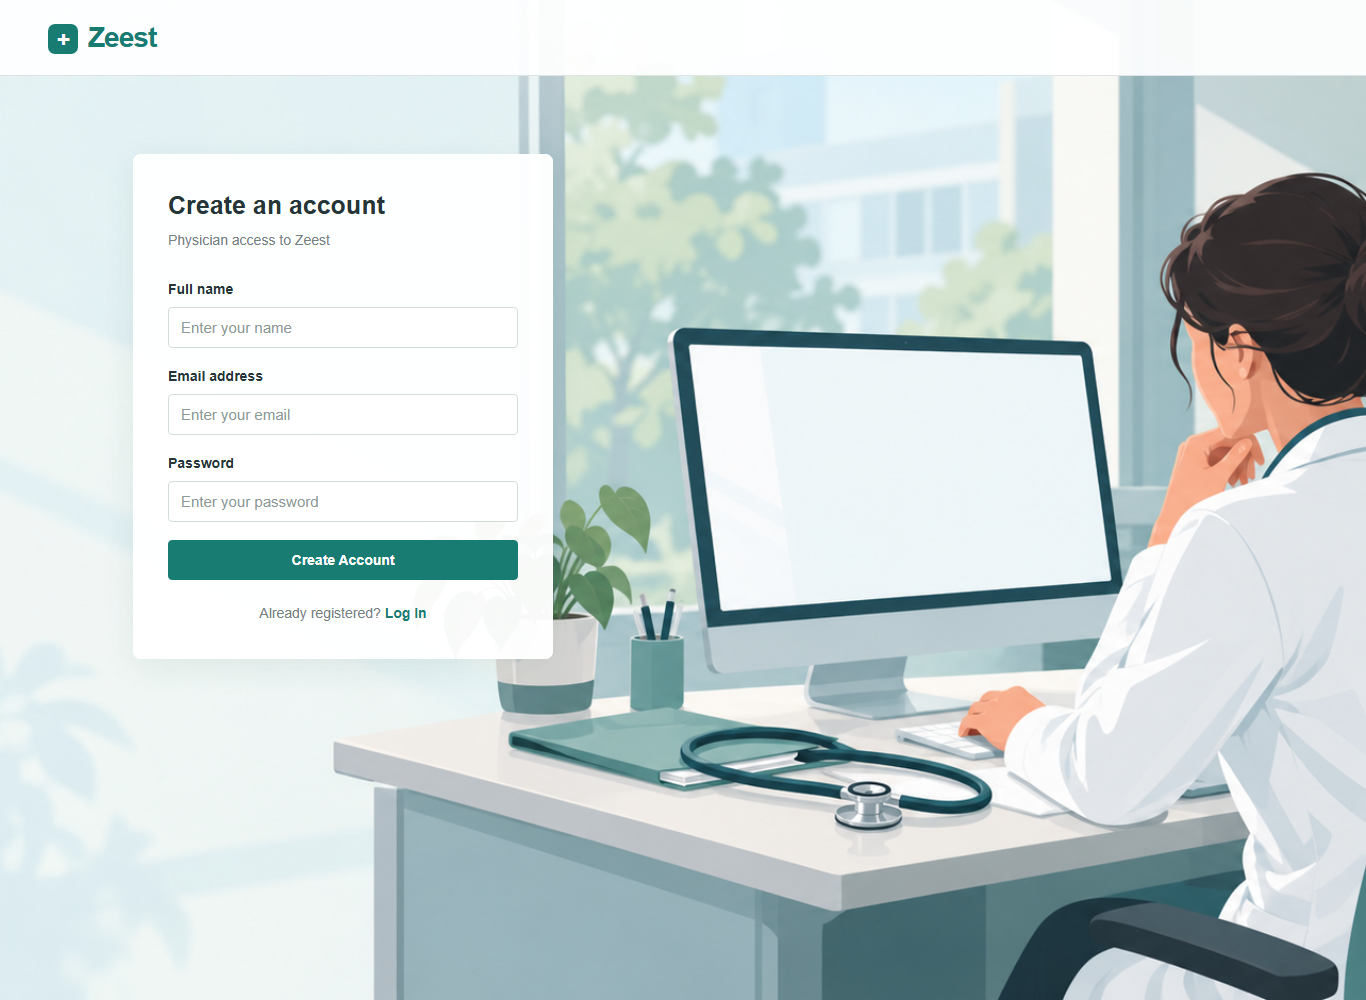
\includegraphics[width=0.96\textwidth,keepaspectratio]{Figures/kashaf_G01_signup.png}
\caption{Physician registration form with name, email and password fields (UC01).}
\label{fig:kashaf:gui-signup}

\centering
\vspace{10pt}
\centering
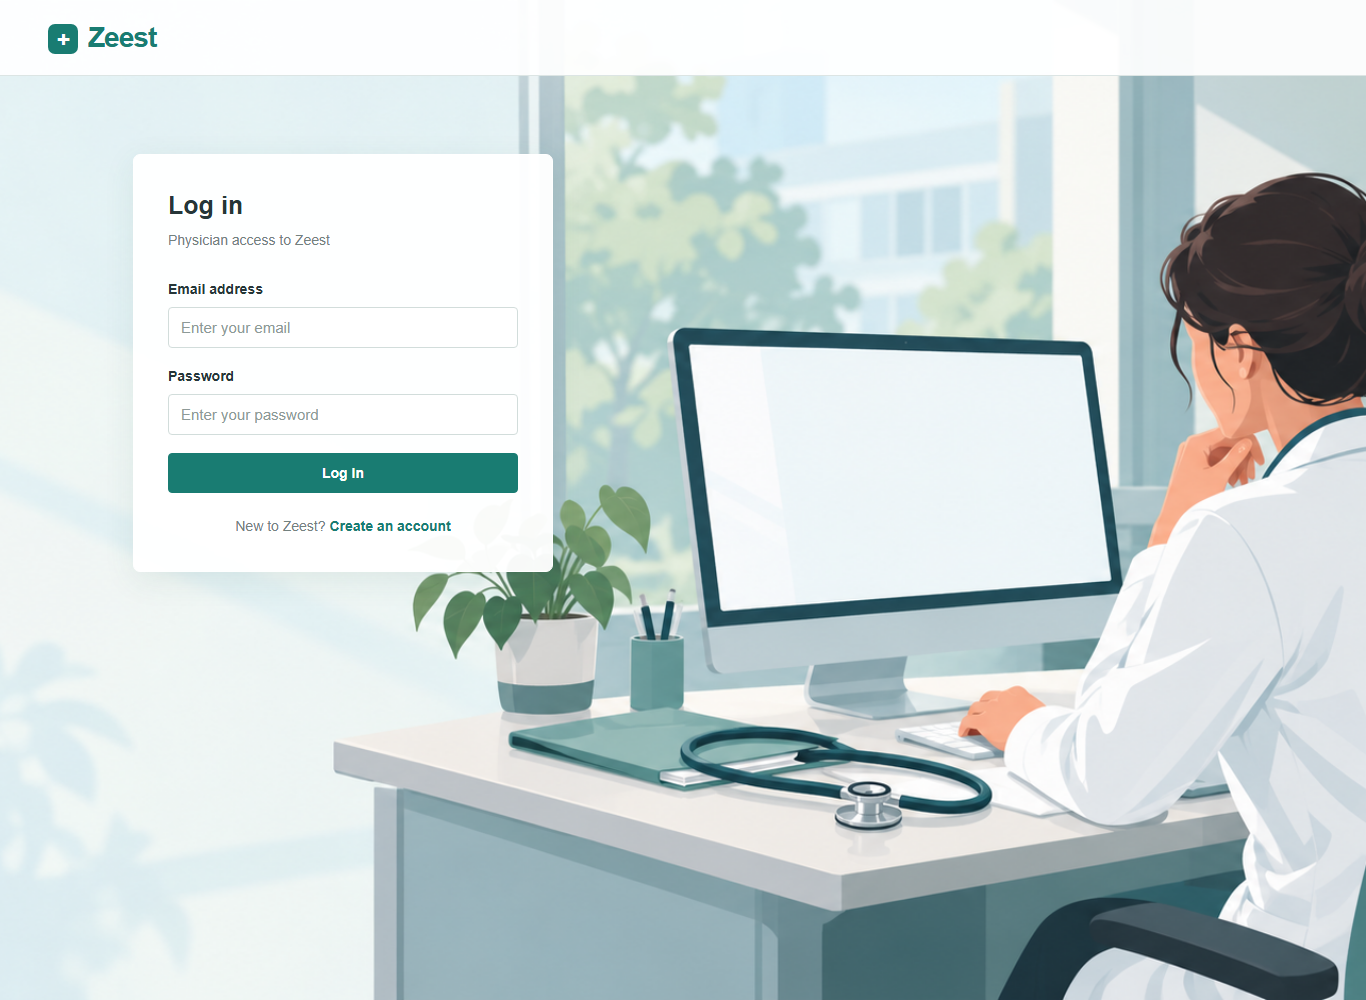
\includegraphics[width=0.96\textwidth,keepaspectratio]{Figures/kashaf_G02_login.png}
\caption{Physician login form and account-access controls (UC02, UC21).}
\label{fig:kashaf:gui-login}
\end{figure}

\begin{figure}[!htbp]
\centering
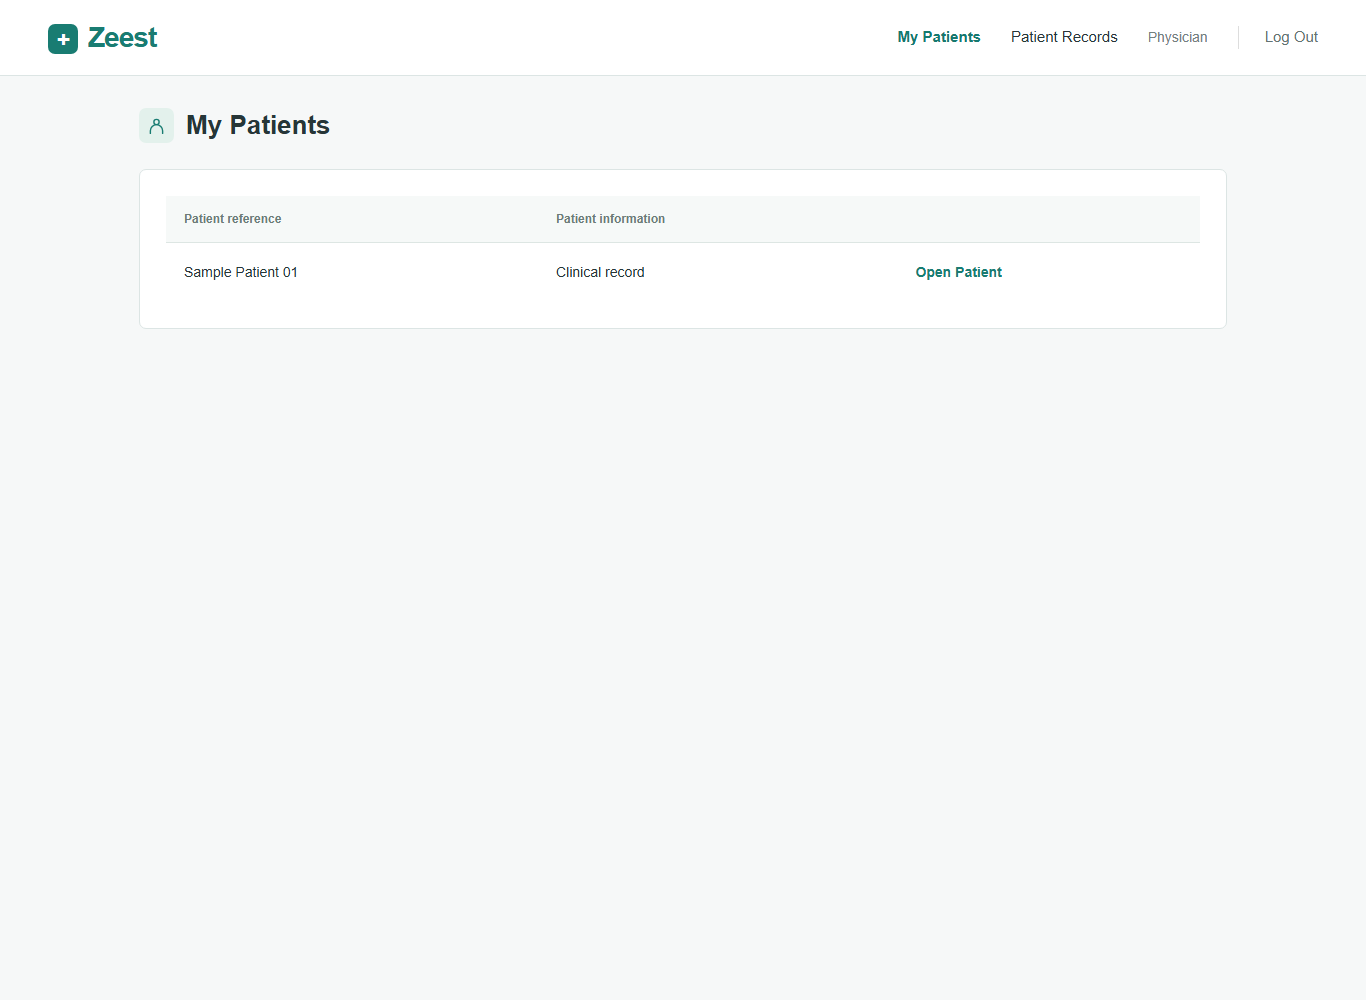
\includegraphics[width=0.96\textwidth,keepaspectratio]{Figures/kashaf_G03_patients.png}
\caption{Physician patient list and selection controls (UC03, UC21).}
\label{fig:kashaf:gui-patients}

\centering
\vspace{10pt}
\centering
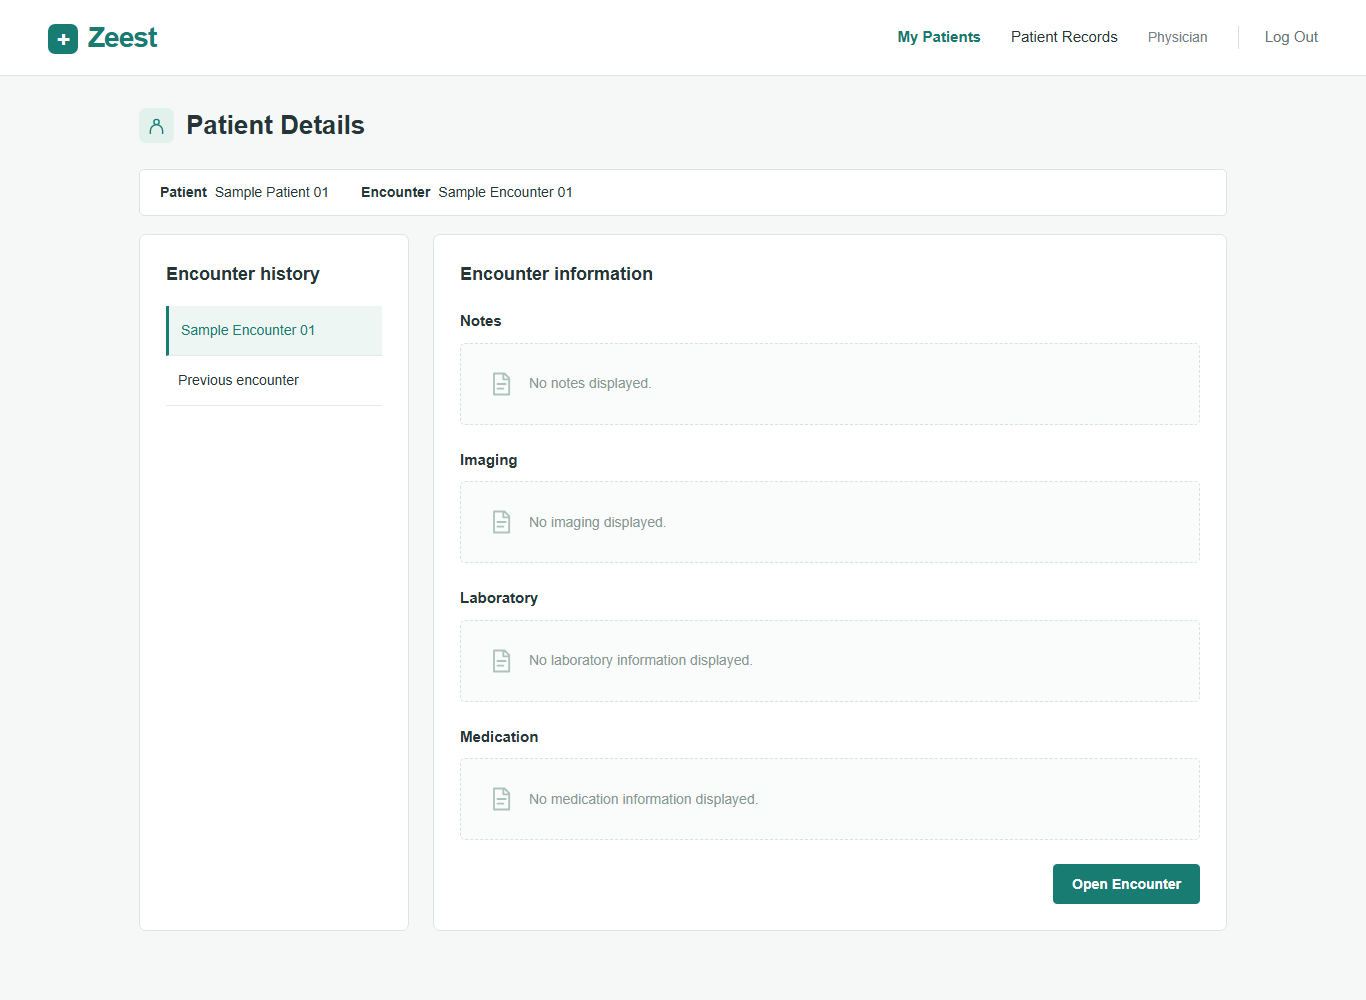
\includegraphics[width=0.96\textwidth,keepaspectratio]{Figures/kashaf_G04_history.png}
\caption{Patient context, history and encounter selection (Physician, UC04--UC06).}
\label{fig:kashaf:gui-history}
\end{figure}

\begin{figure}[!htbp]
\centering
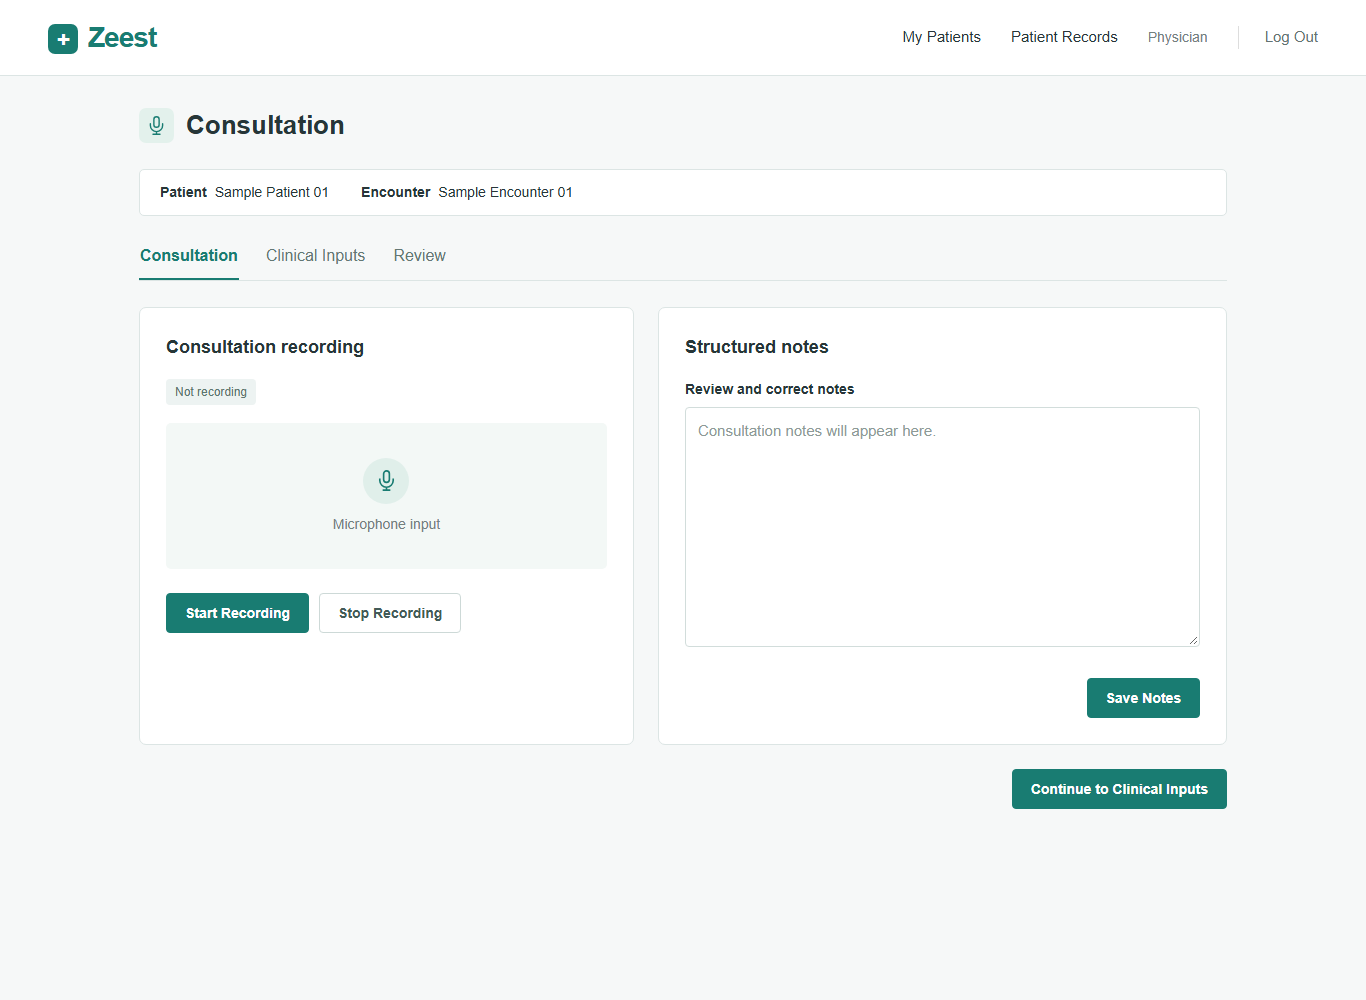
\includegraphics[width=0.96\textwidth,height=.88\textheight,keepaspectratio]{Figures/kashaf_G05_consultation.png}
\caption{Consultation recording controls and editable notes (Physician, UC07--UC08).}
\label{fig:kashaf:gui-consultation}

\centering
\end{figure}

\begin{figure}[!htbp]
\centering
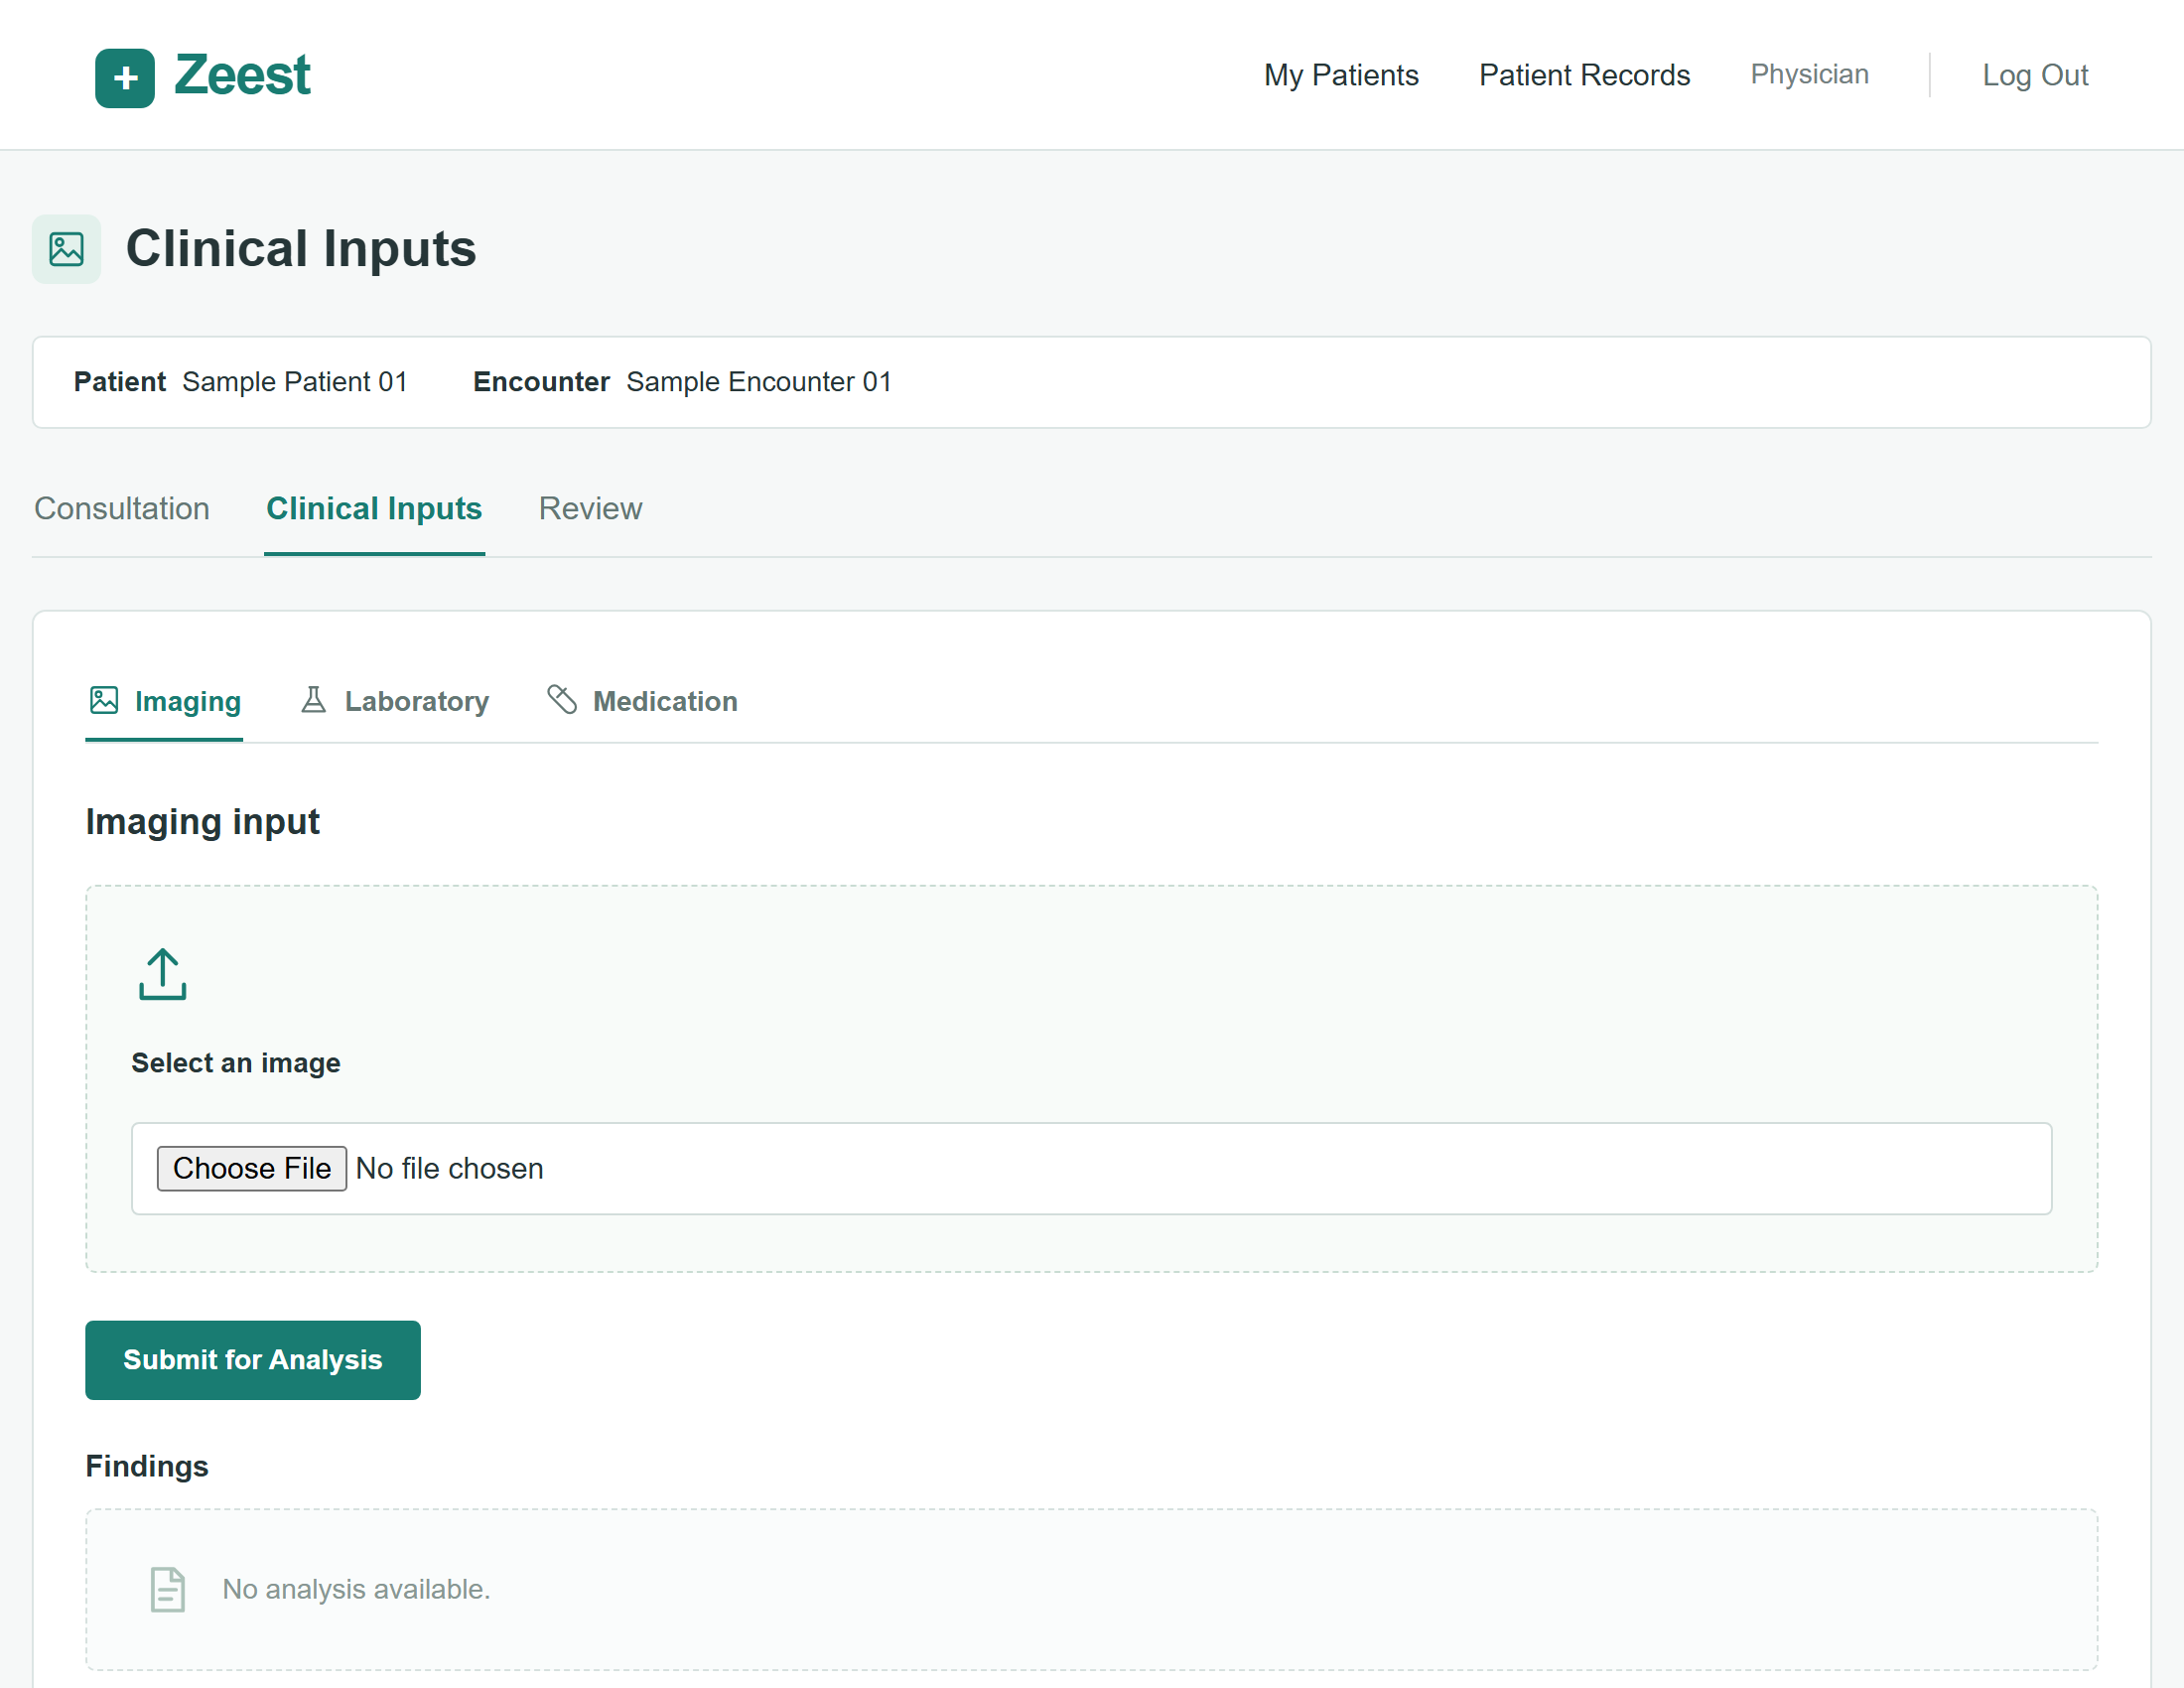
\includegraphics[width=0.96\textwidth,height=.88\textheight,keepaspectratio]{Figures/kashaf_G06_imaging.png}
\caption{Imaging upload and findings area (Physician, UC09, UC12).}
\label{fig:kashaf:gui-imaging}
\end{figure}

\begin{figure}[!htbp]
\centering
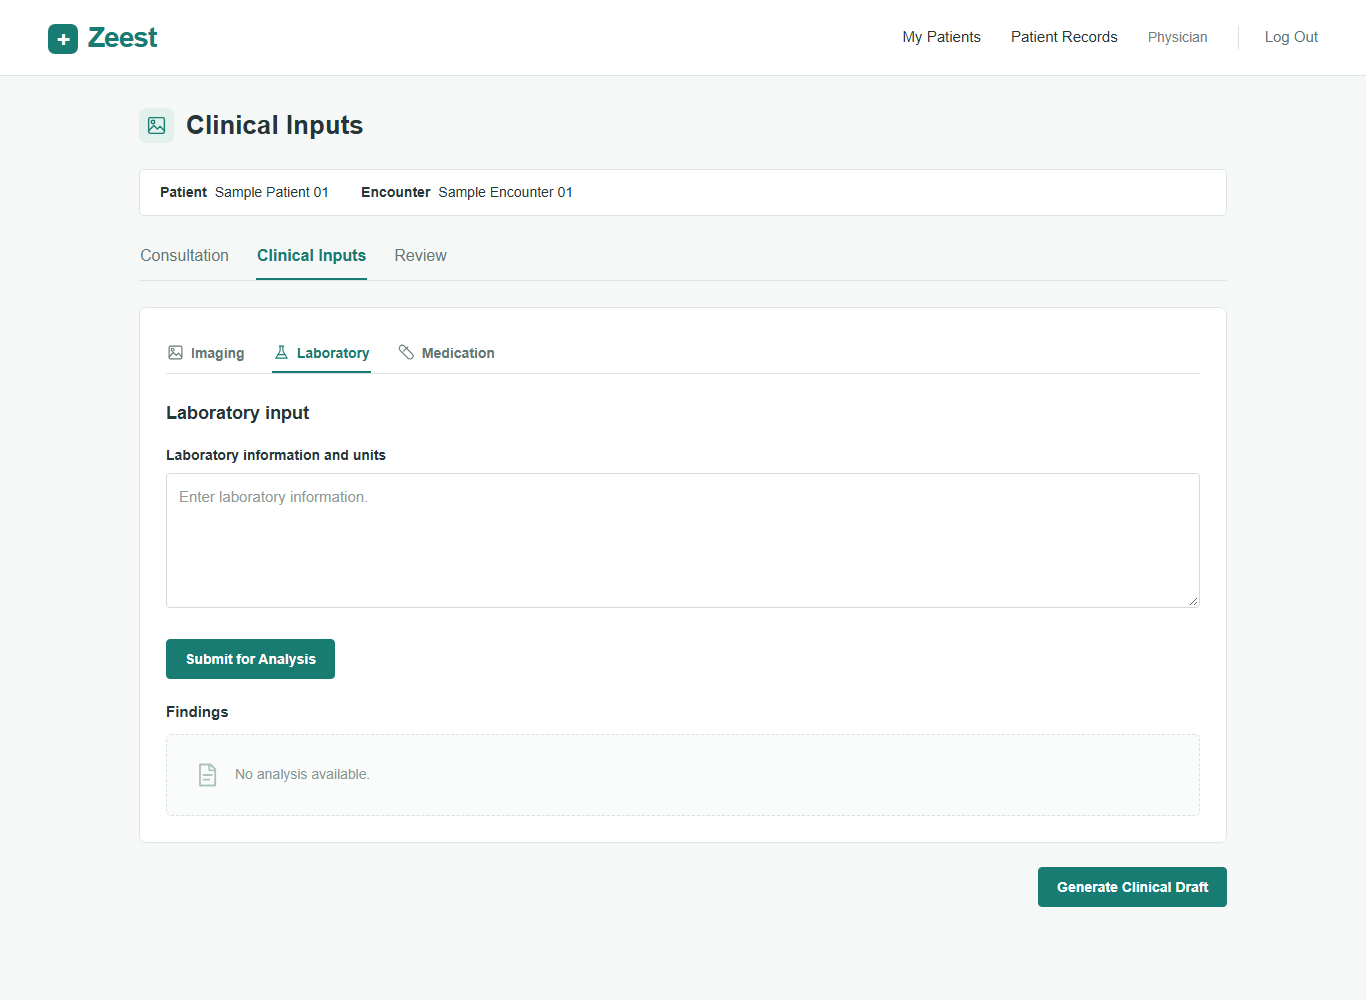
\includegraphics[width=0.96\textwidth,height=.88\textheight,keepaspectratio]{Figures/kashaf_G07_laboratory.png}
\caption{Laboratory input and findings area (Physician, UC10, UC12).}
\label{fig:kashaf:gui-laboratory}

\centering
\end{figure}

\begin{figure}[!htbp]
\centering
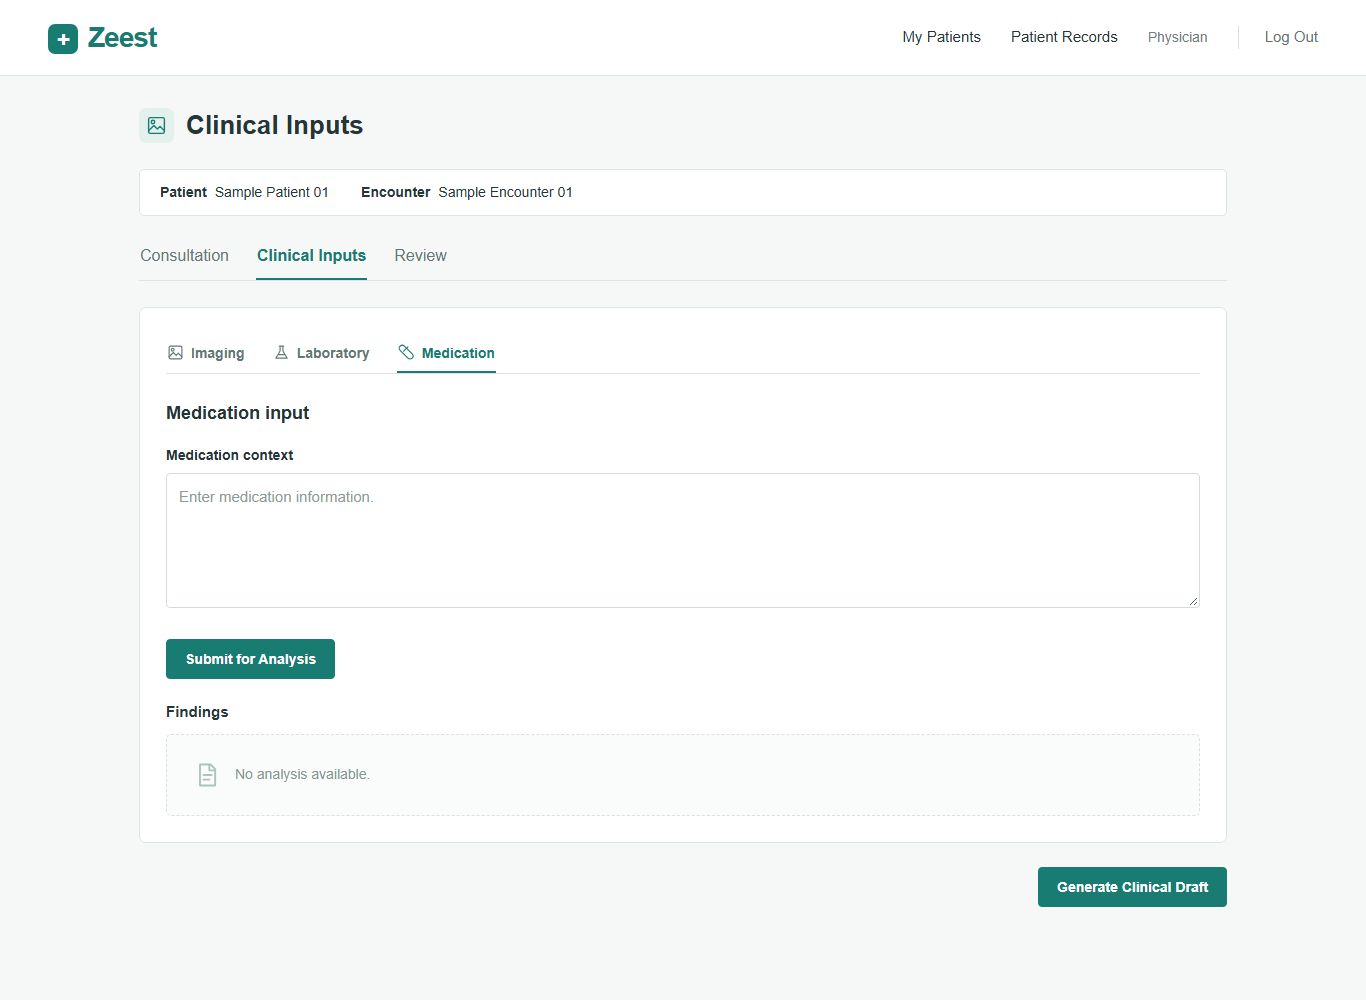
\includegraphics[width=0.96\textwidth,height=.88\textheight,keepaspectratio]{Figures/kashaf_G08_medication.png}
\caption{Medication input and findings area (Physician, UC11, UC12).}
\label{fig:kashaf:gui-medication}
\end{figure}

\begin{figure}[!htbp]
\centering
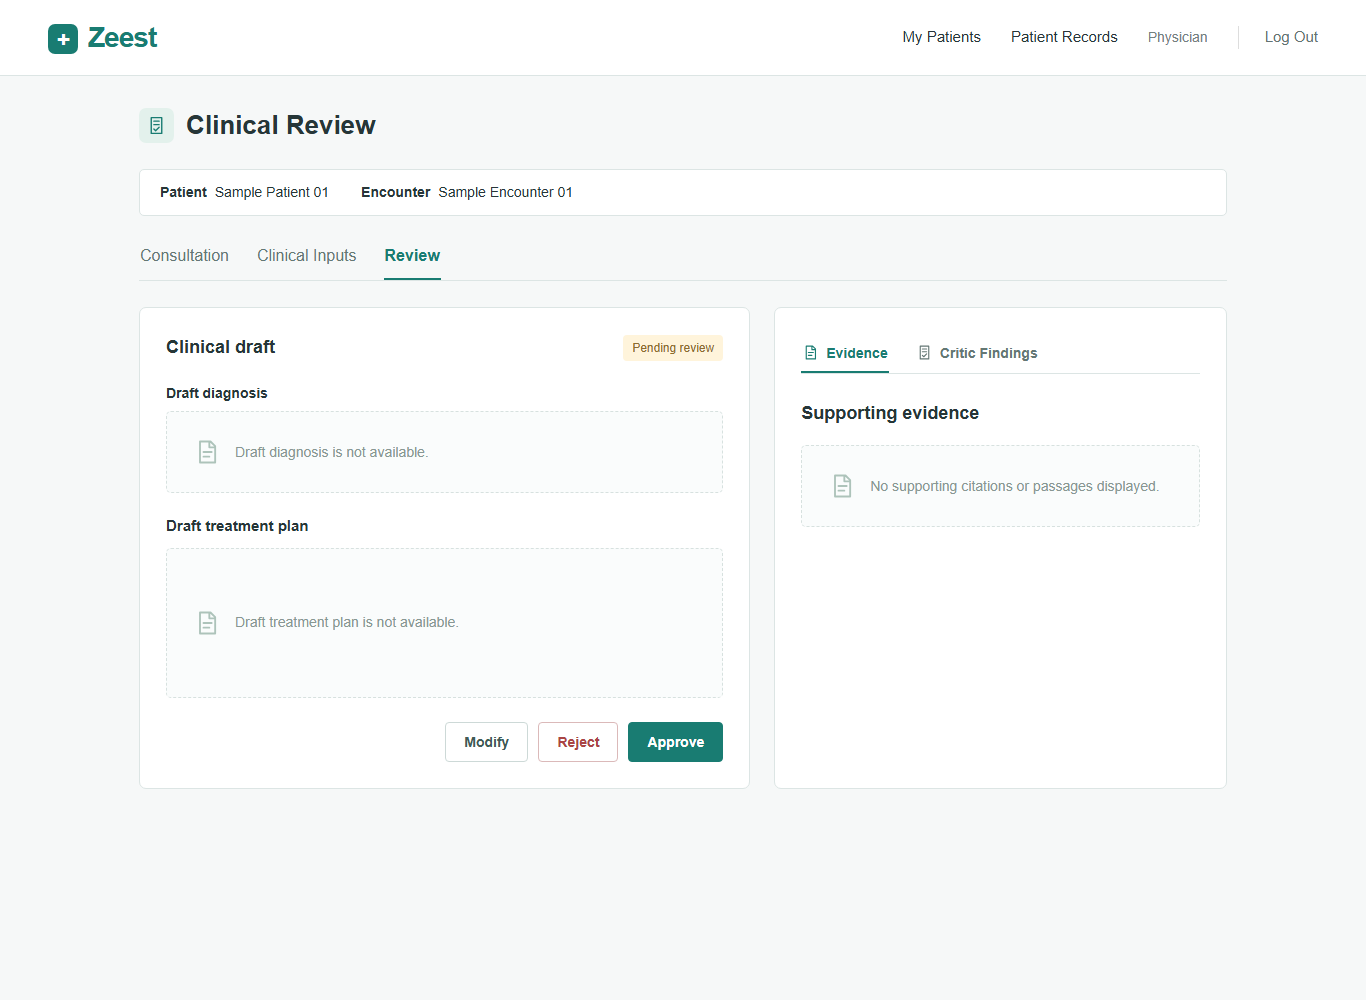
\includegraphics[width=0.96\textwidth,keepaspectratio]{Figures/kashaf_G09_review.png}
\caption{Clinical draft and supporting evidence tabs (Physician, UC13--UC14).}
\label{fig:kashaf:gui-review}

\centering
\vspace{10pt}
\centering
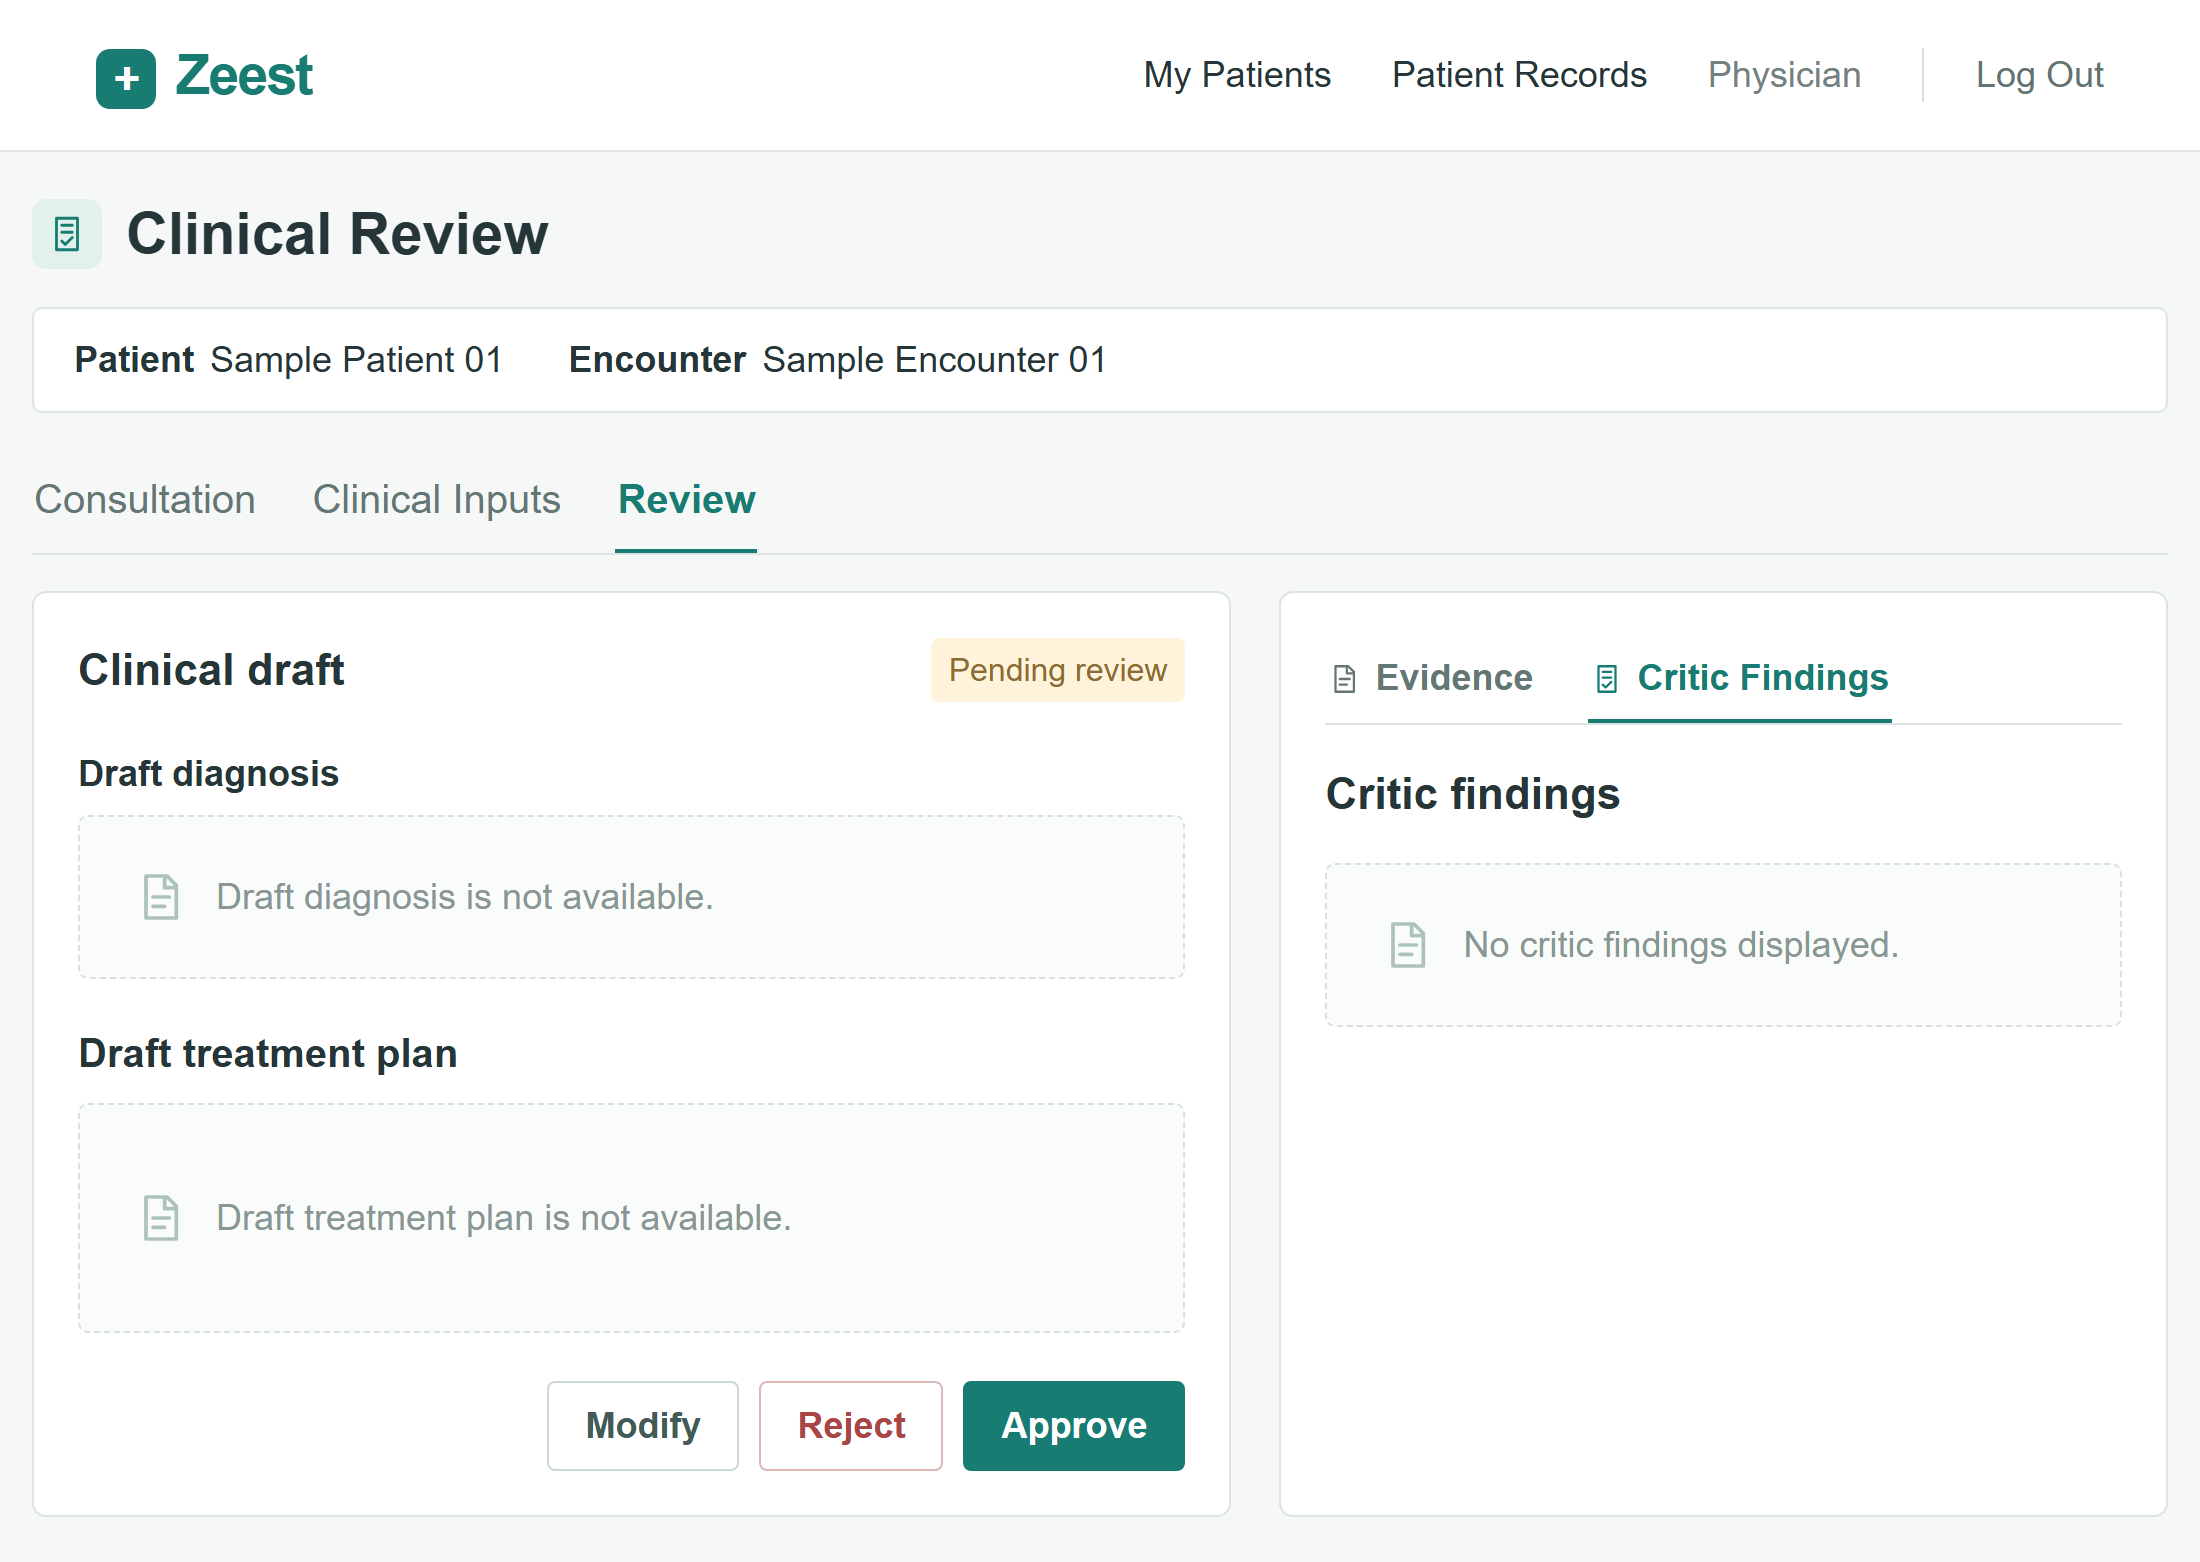
\includegraphics[width=0.96\textwidth,keepaspectratio]{Figures/kashaf_G10_critic.png}
\caption{Critic findings beside the clinical draft (Physician, UC15).}
\label{fig:kashaf:gui-critic}
\end{figure}

\begin{figure}[!htbp]
\centering
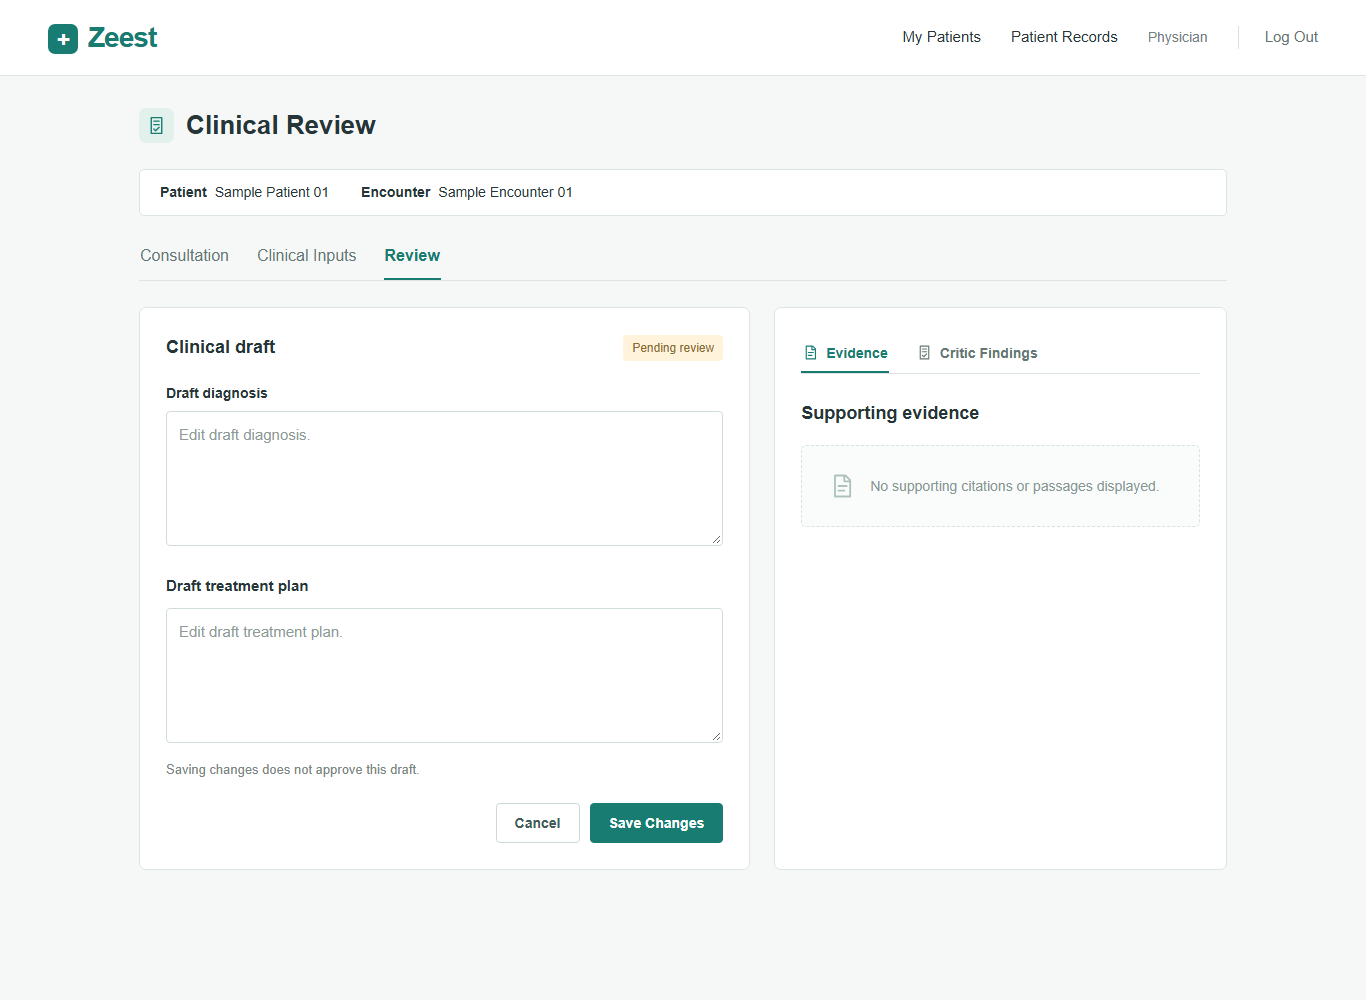
\includegraphics[width=0.96\textwidth,height=.88\textheight,keepaspectratio]{Figures/kashaf_G11_modify.png}
\caption{Draft revision editor and save controls (Physician, UC16).}
\label{fig:kashaf:gui-modify}

\centering
\end{figure}

\begin{figure}[!htbp]
\centering
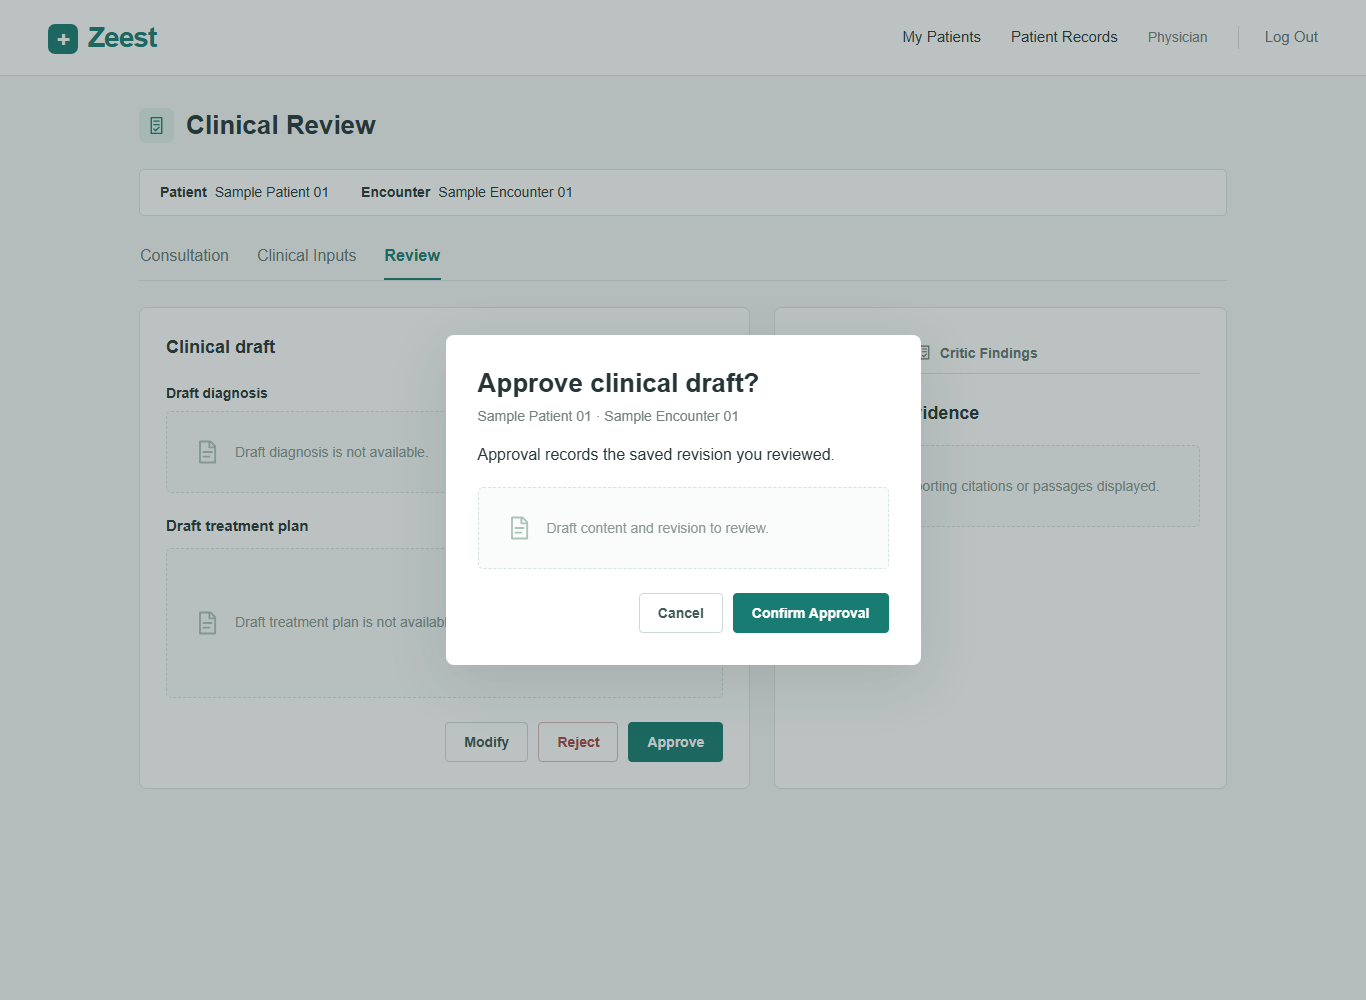
\includegraphics[width=0.96\textwidth,height=.88\textheight,keepaspectratio]{Figures/kashaf_G12_approve.png}
\caption{Confirmation dialog for explicit draft approval (Physician, UC17).}
\label{fig:kashaf:gui-approve}
\end{figure}

\begin{figure}[!htbp]
\centering
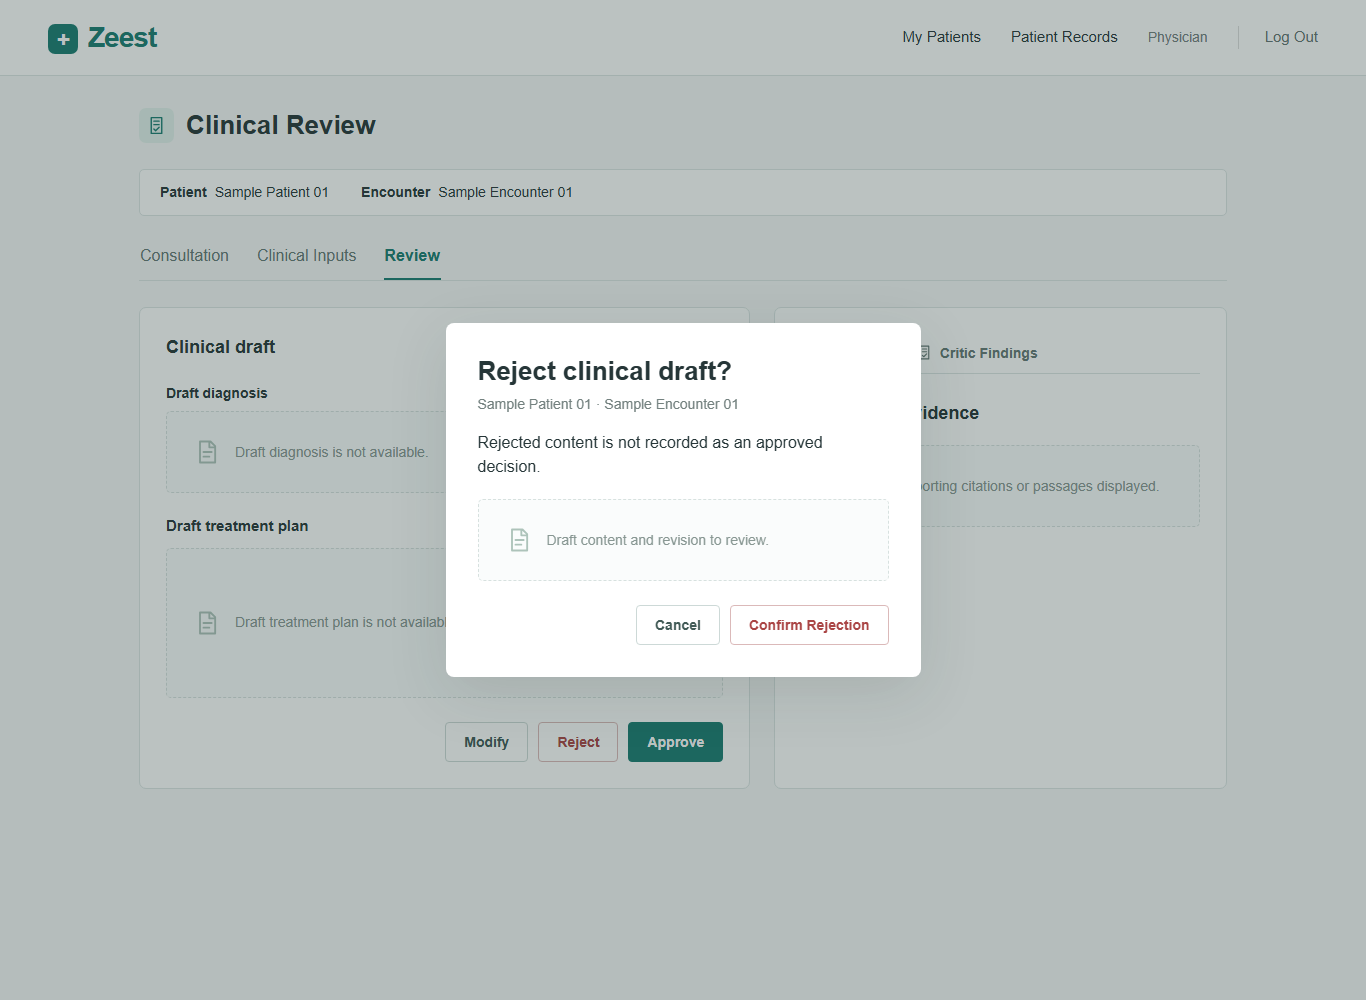
\includegraphics[width=0.96\textwidth,keepaspectratio]{Figures/kashaf_G13_reject.png}
\caption{Confirmation dialog for draft rejection (Physician, UC18).}
\label{fig:kashaf:gui-reject}

\centering
\vspace{10pt}
\centering
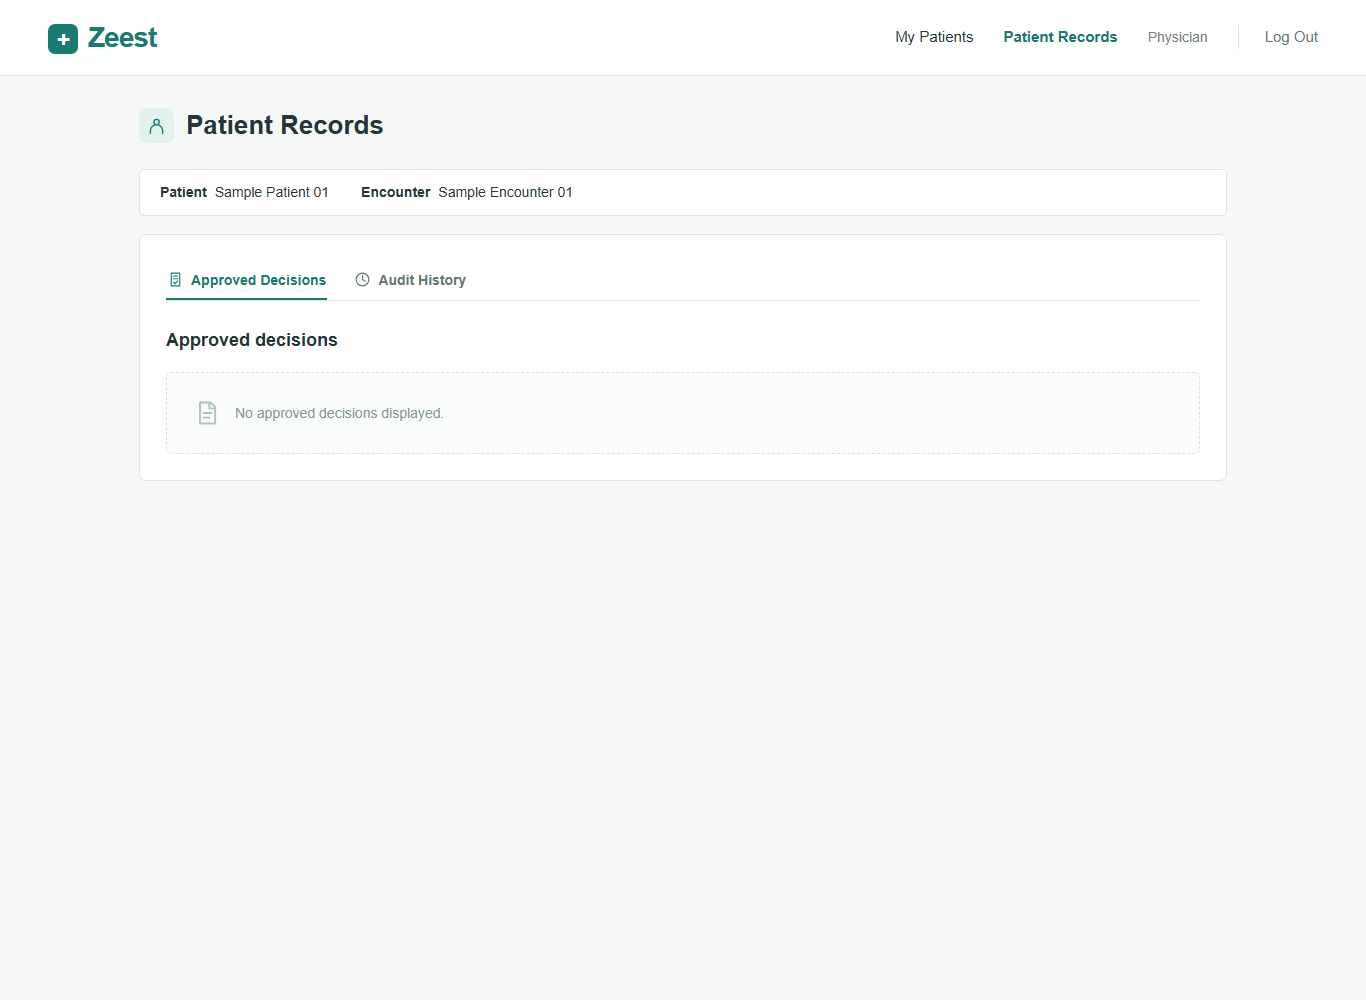
\includegraphics[width=0.96\textwidth,keepaspectratio]{Figures/kashaf_G14_decisions.png}
\caption{Selected encounter approved-decision view (Physician, UC19).}
\label{fig:kashaf:gui-decisions}
\end{figure}

\begin{figure}[!htbp]
\centering
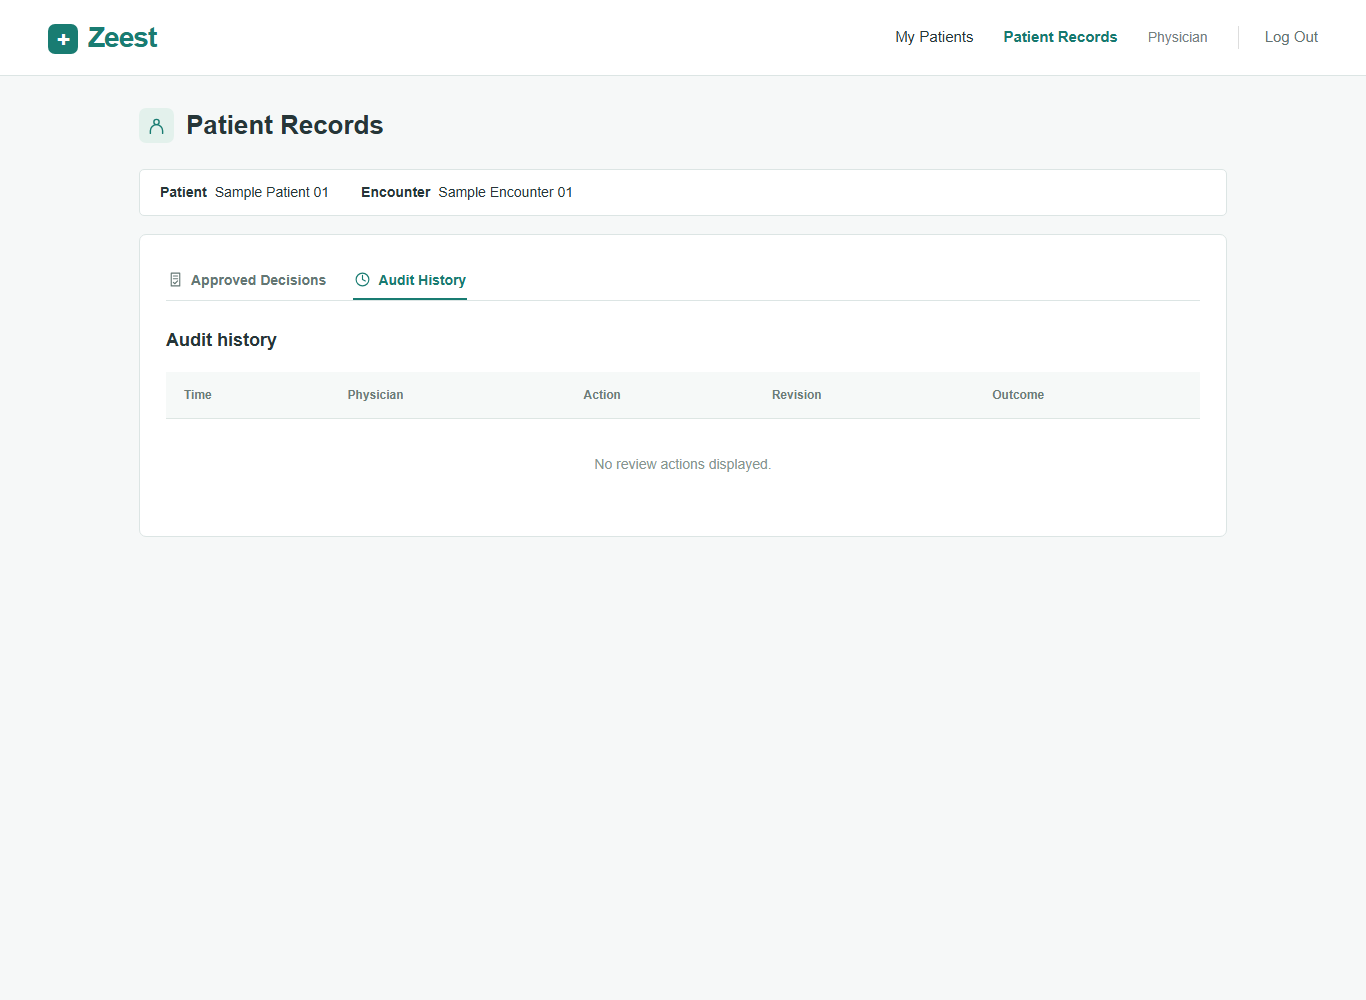
\includegraphics[width=0.96\textwidth,keepaspectratio]{Figures/kashaf_G15_audit.png}
\caption{Encounter review-action history table (Physician, UC20).}
\label{fig:kashaf:gui-audit}

\centering
\vspace{10pt}
\centering
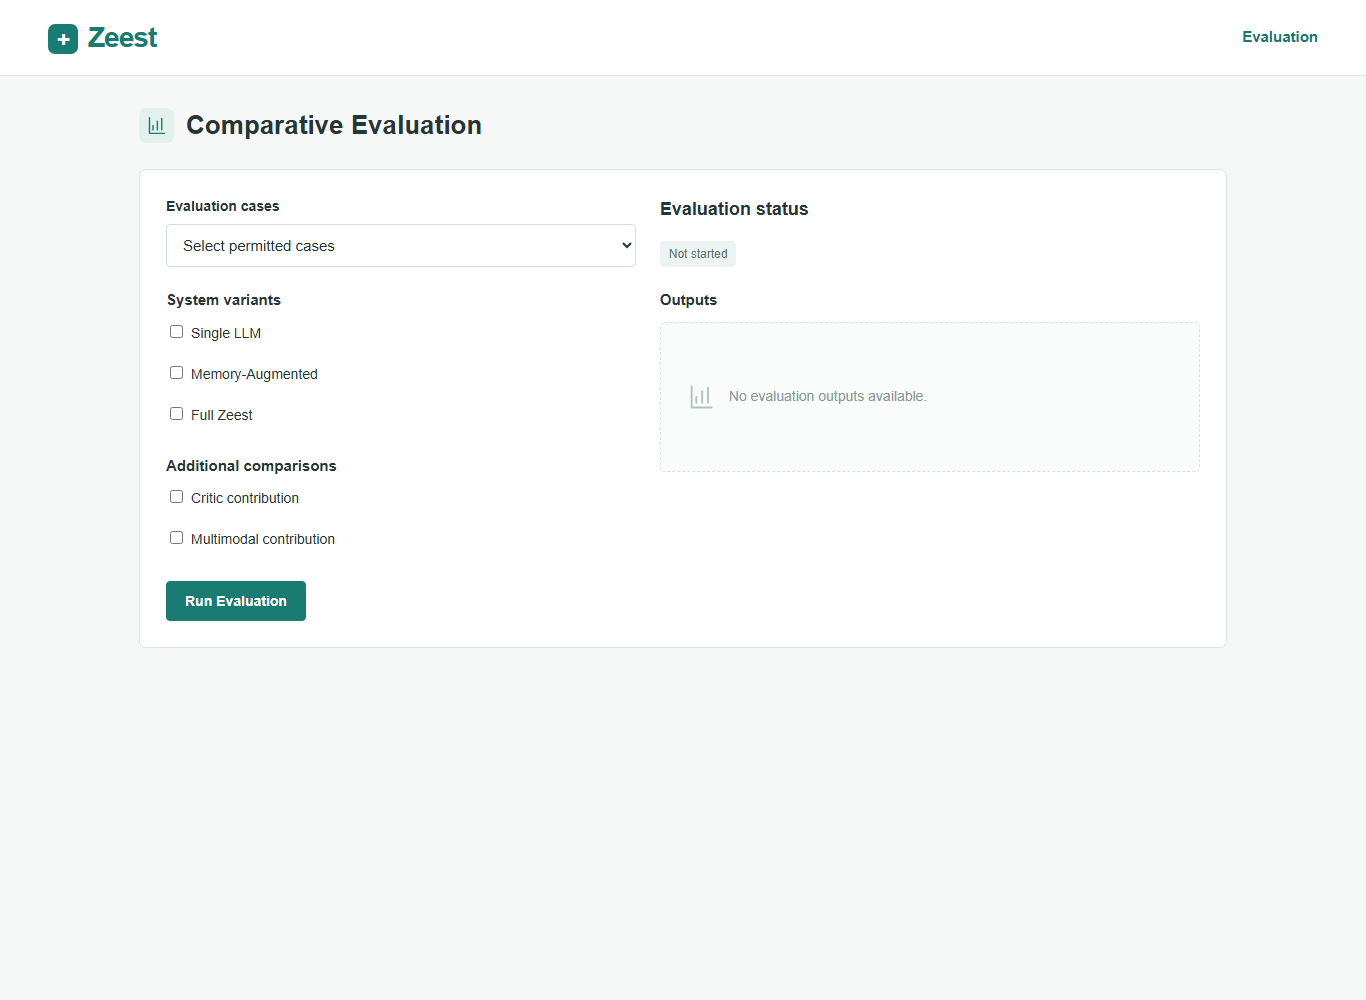
\includegraphics[width=0.96\textwidth,keepaspectratio]{Figures/kashaf_G16_evaluation.png}
\caption{Case, variant and run controls for comparative evaluation (Research team, UC22).}
\label{fig:kashaf:gui-evaluation}
\end{figure}


\section{Database Design}

The logical design separates physician accounts, patient ownership, clinical information, generated drafts and accepted decisions. Each patient has one responsible physician, and encounters inherit that ownership through the patient. Clinical case inputs retain saved revisions, allowing findings and draft preparation to identify their exact source content. Draft revisions keep diagnosis and treatment text distinct from approval actions and accepted decisions. Retrieved evidence and critic reviews refer to the assessed revision. Semantic representations originate from an input revision or an approved decision. Separate evaluation records connect permitted cases, run settings and recorded outputs. These relationships preserve continuity, source traceability and physician authority across the defined clinical workflow. The schema is a logical design rather than an implemented database. Patient ownership and revision consistency require explicit validation alongside foreign keys. Model-dependent vector dimensions remain configuration choices, and evaluation outputs represent records to be populated after actual runs rather than supplied numerical findings.

\subsection{ER Diagram}

Figure~\ref{fig:kashaf:er} presents the complete conceptual model with entities, relationship diamonds and attribute ovals together. Dashed regions group accounts and clinical information, drafts and supporting evidence, physician review and memory, and comparative evaluation. Blue rectangles identify entities, green ovals identify attributes, and amber diamonds identify named relationships. Primary keys are underlined and foreign keys are marked FK. Cardinalities express ownership and record associations, while revision keys preserve the exact content used or reviewed. Figures~\ref{fig:kashaf:er-clinical}, \ref{fig:kashaf:er-drafts}, \ref{fig:kashaf:er-review} and~\ref{fig:kashaf:er-evaluation} enlarge the same regions; cross-region relationships remain visible in the complete model. The grouped enlargements retain the same entity and relationship names as the overview, allowing attributes and cardinalities to be read at print size. Login and registration are account operations rather than separate persistent clinical entities. Evaluation links remain separate from clinical decisions, so a comparative output cannot become an approved patient record merely because it was saved. Region enlargements preserve the same underlying schema.

\begin{figure}[!htbp]
\centering
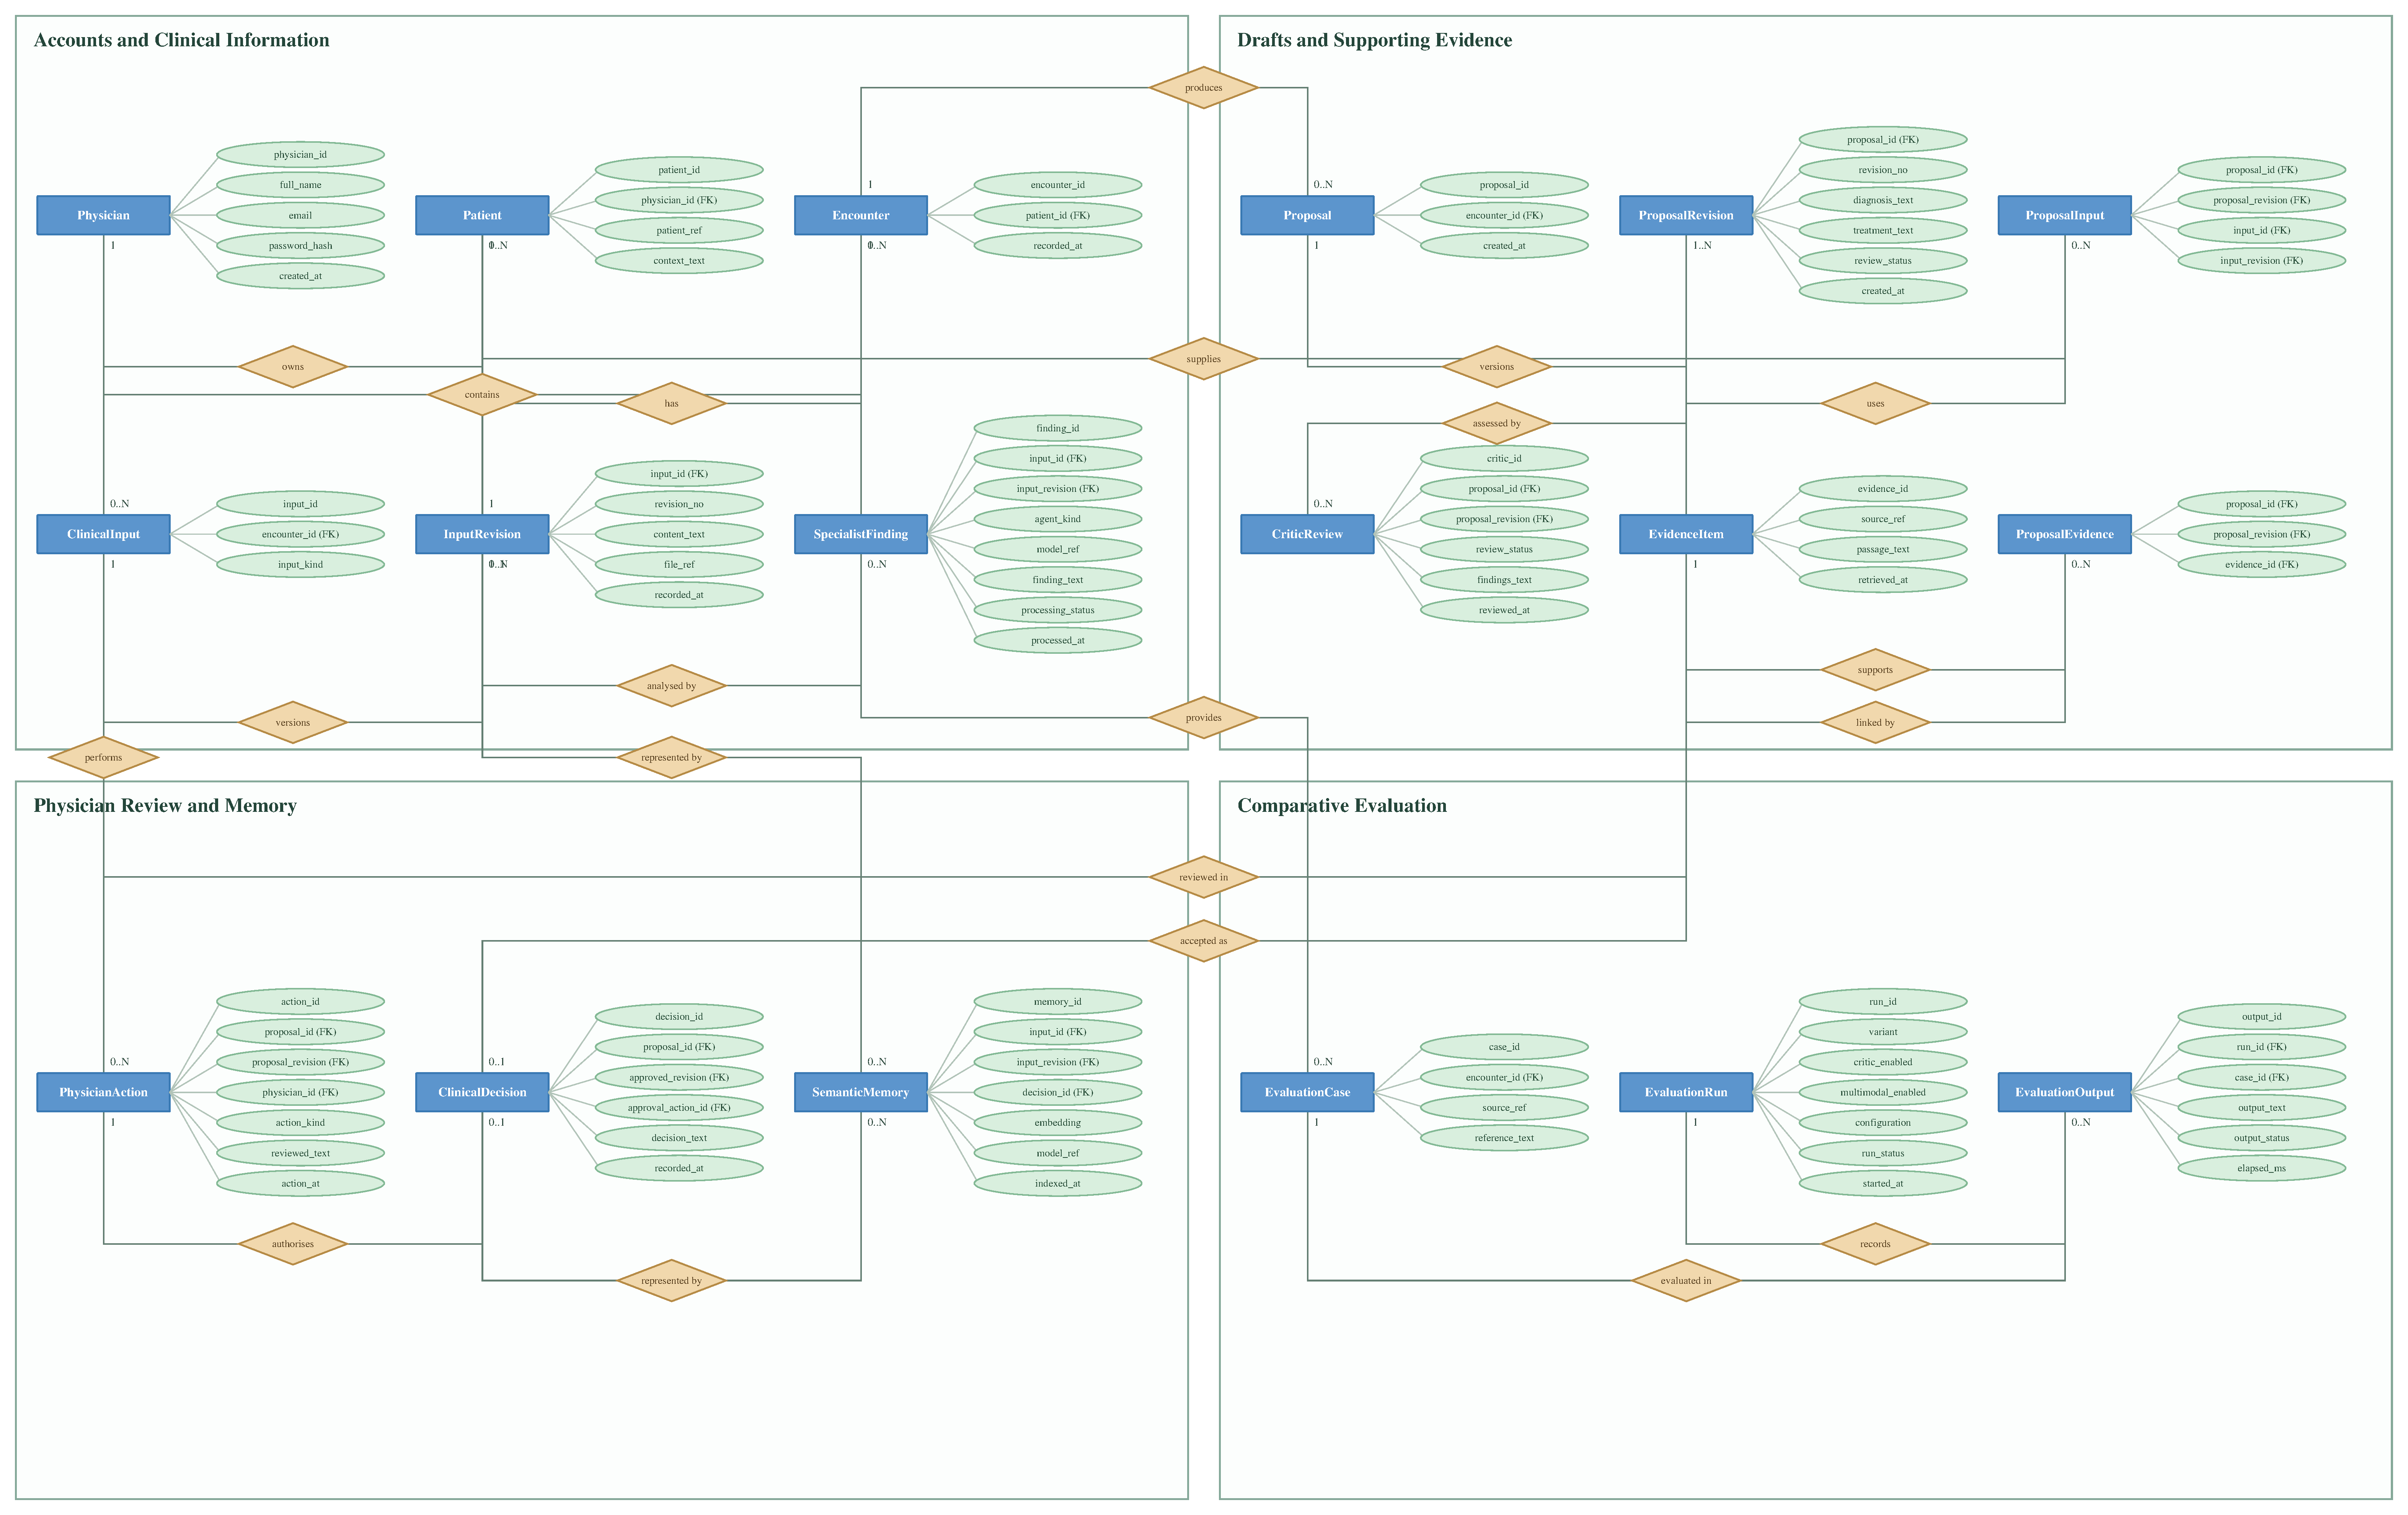
\includegraphics[width=\textwidth,height=0.80\textheight,keepaspectratio]{Figures/kashaf_D03_conceptual_combined.pdf}
\caption{Complete grouped conceptual ER model with entity, attribute and relationship symbols.}
\label{fig:kashaf:er}
\end{figure}

\begin{figure}[!htbp]
\centering
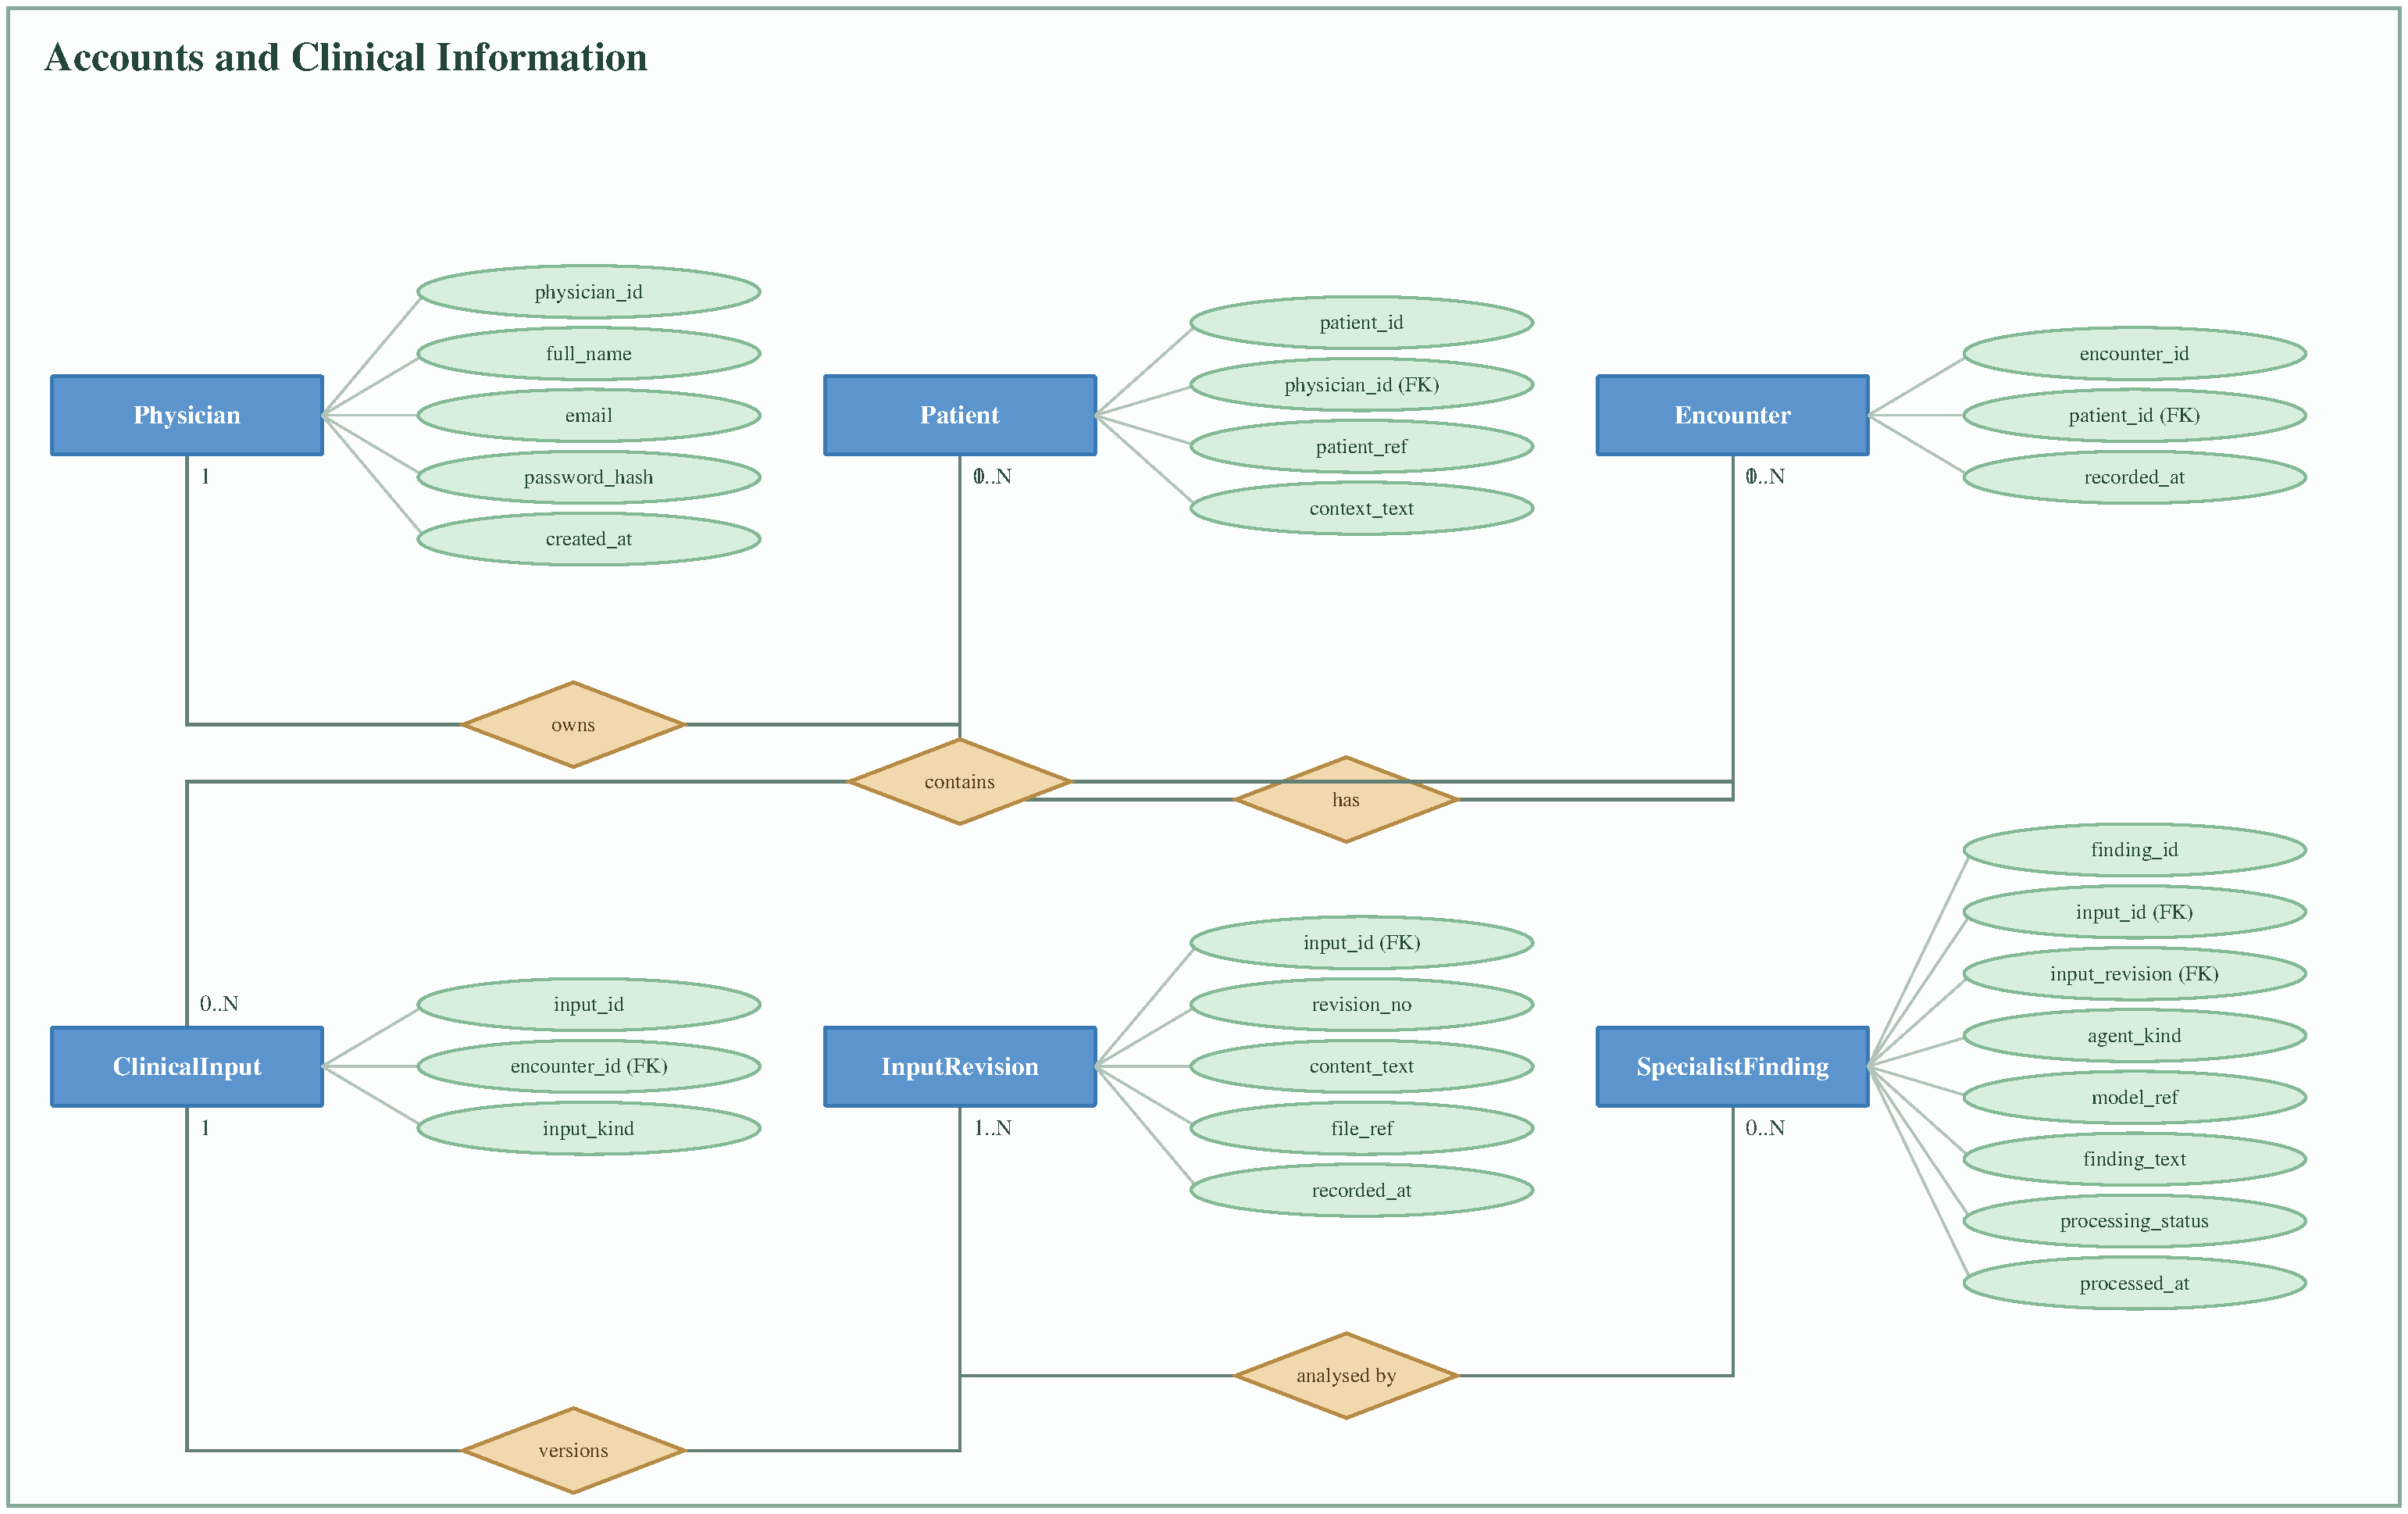
\includegraphics[width=\textwidth,height=0.80\textheight,keepaspectratio]{Figures/kashaf_D03_combined_clinical.pdf}
\caption{Accounts and clinical sources with attributes and relationship cardinalities.}
\label{fig:kashaf:er-clinical}
\end{figure}

\begin{figure}[!htbp]
\centering
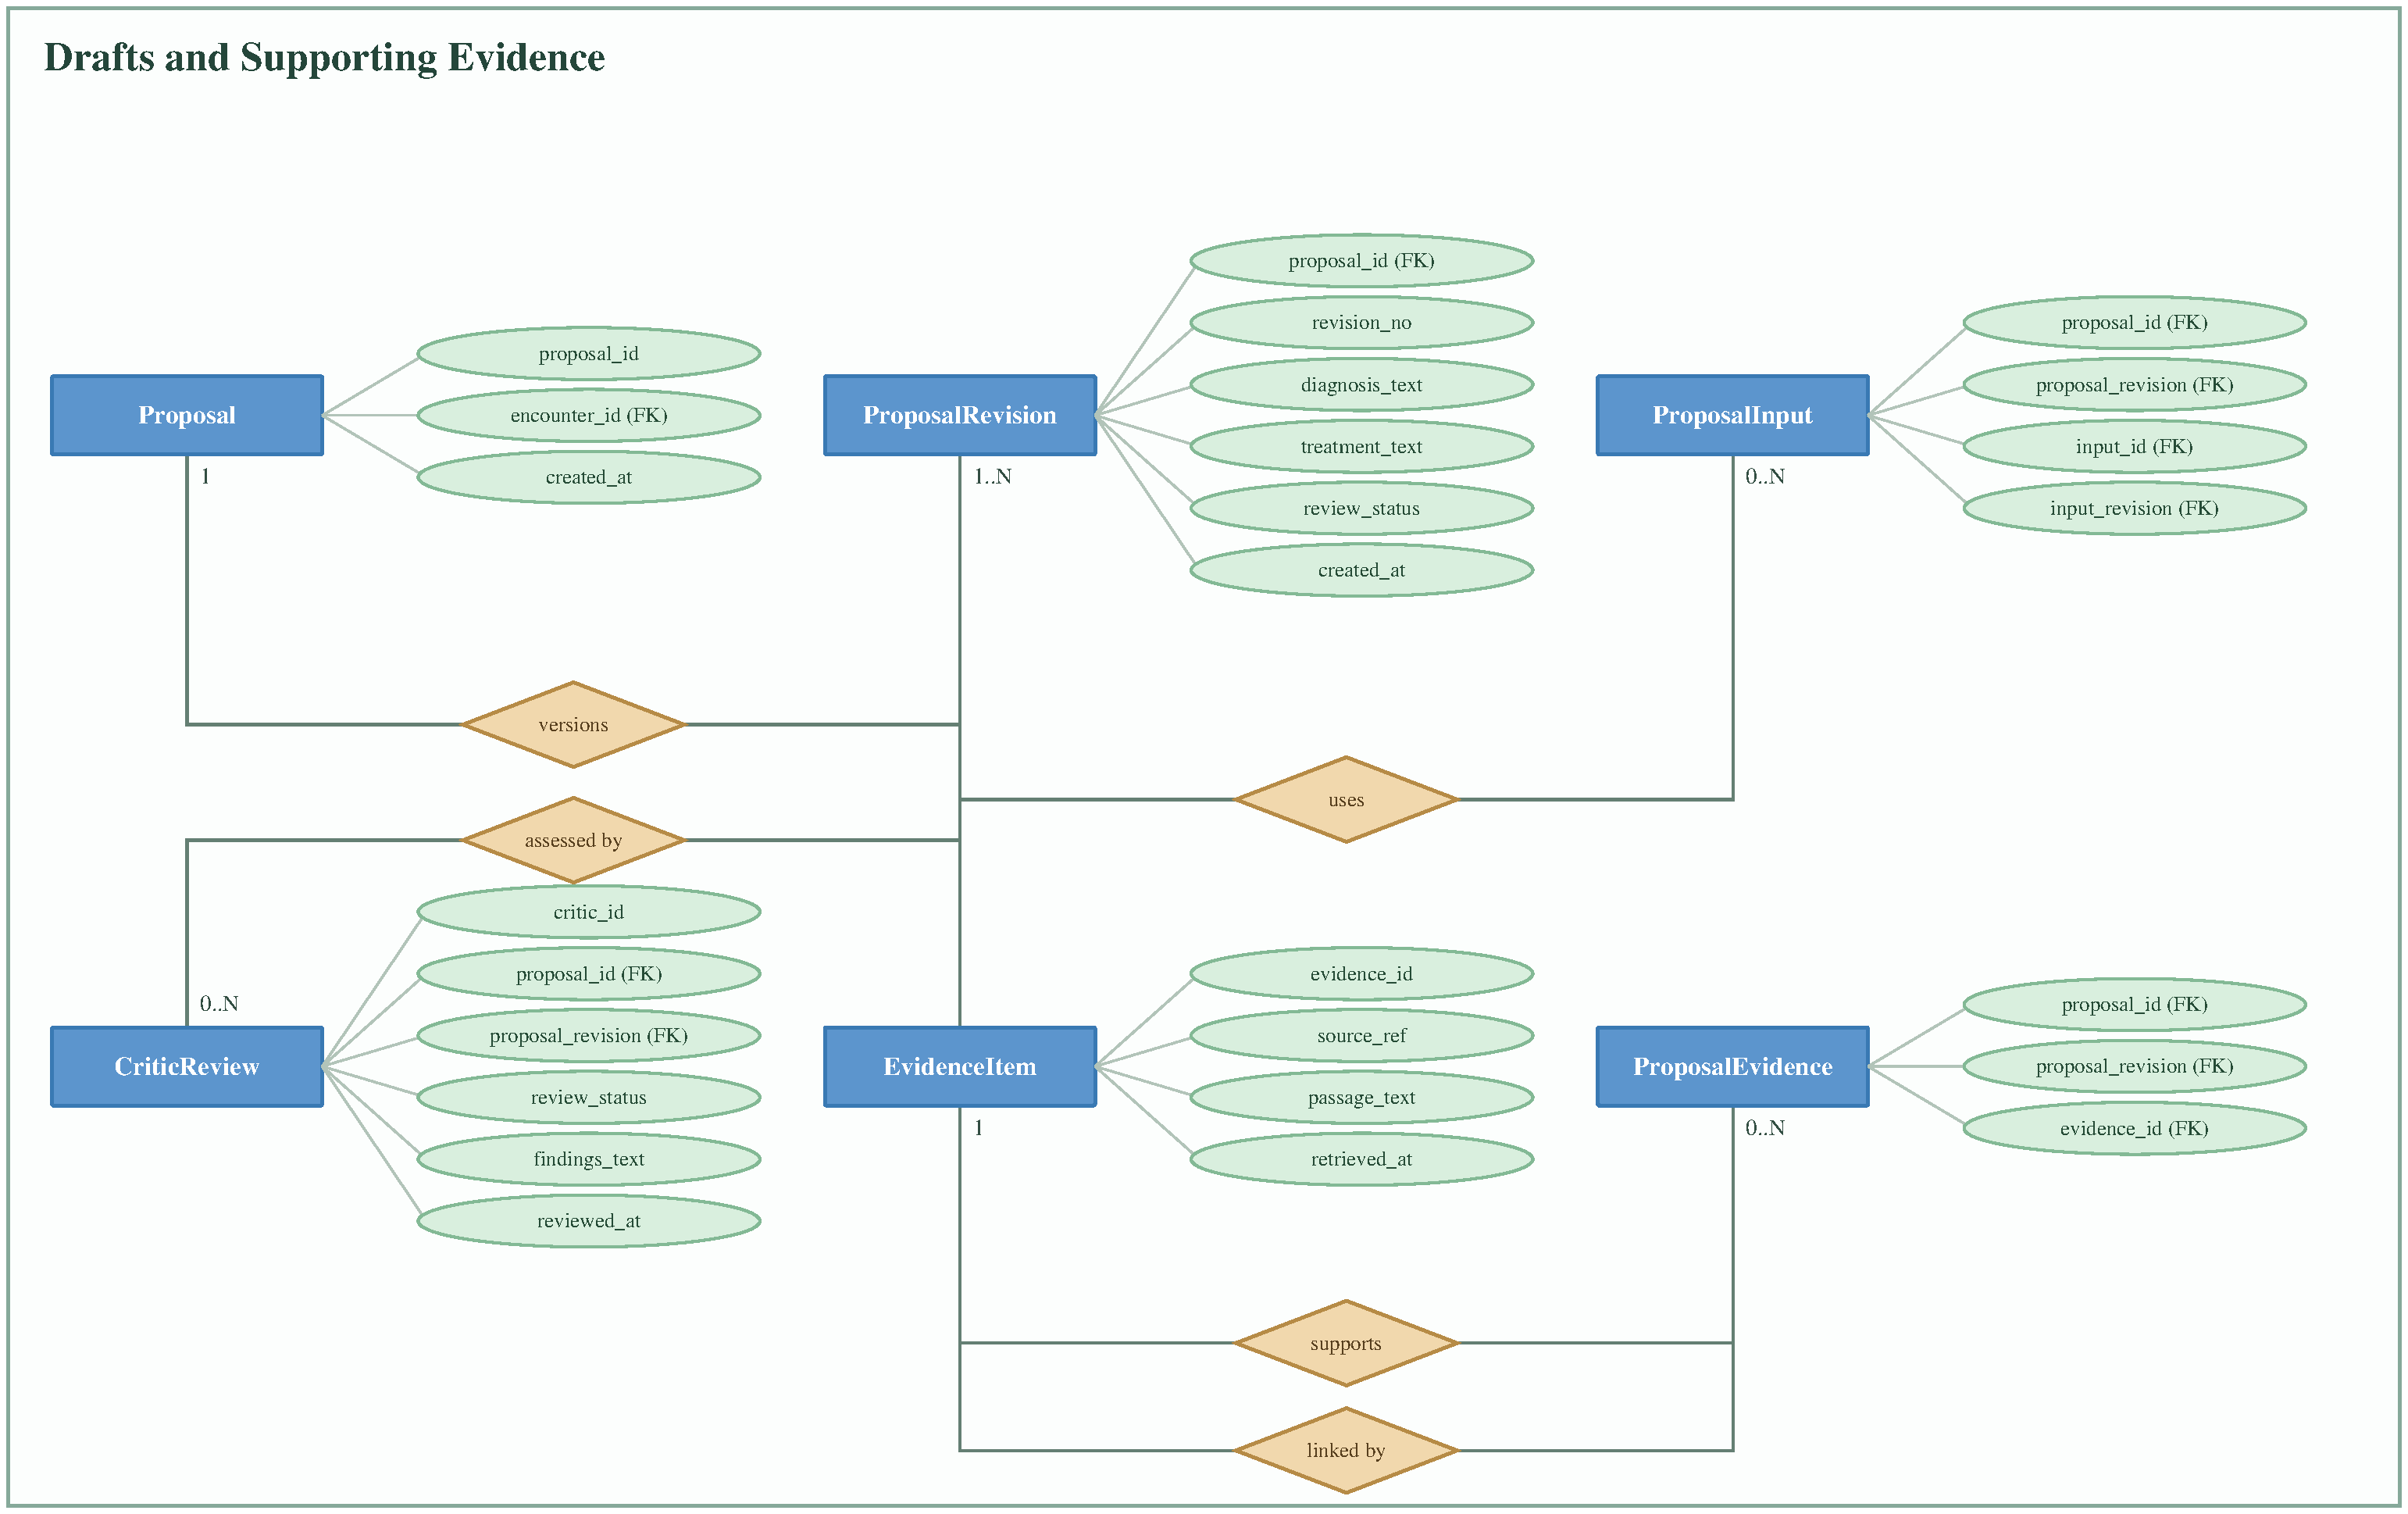
\includegraphics[width=\textwidth,height=0.80\textheight,keepaspectratio]{Figures/kashaf_D03_combined_drafts.pdf}
\caption{Draft revisions, evidence and critic review with attributes and relationships.}
\label{fig:kashaf:er-drafts}
\end{figure}

\begin{figure}[!htbp]
\centering
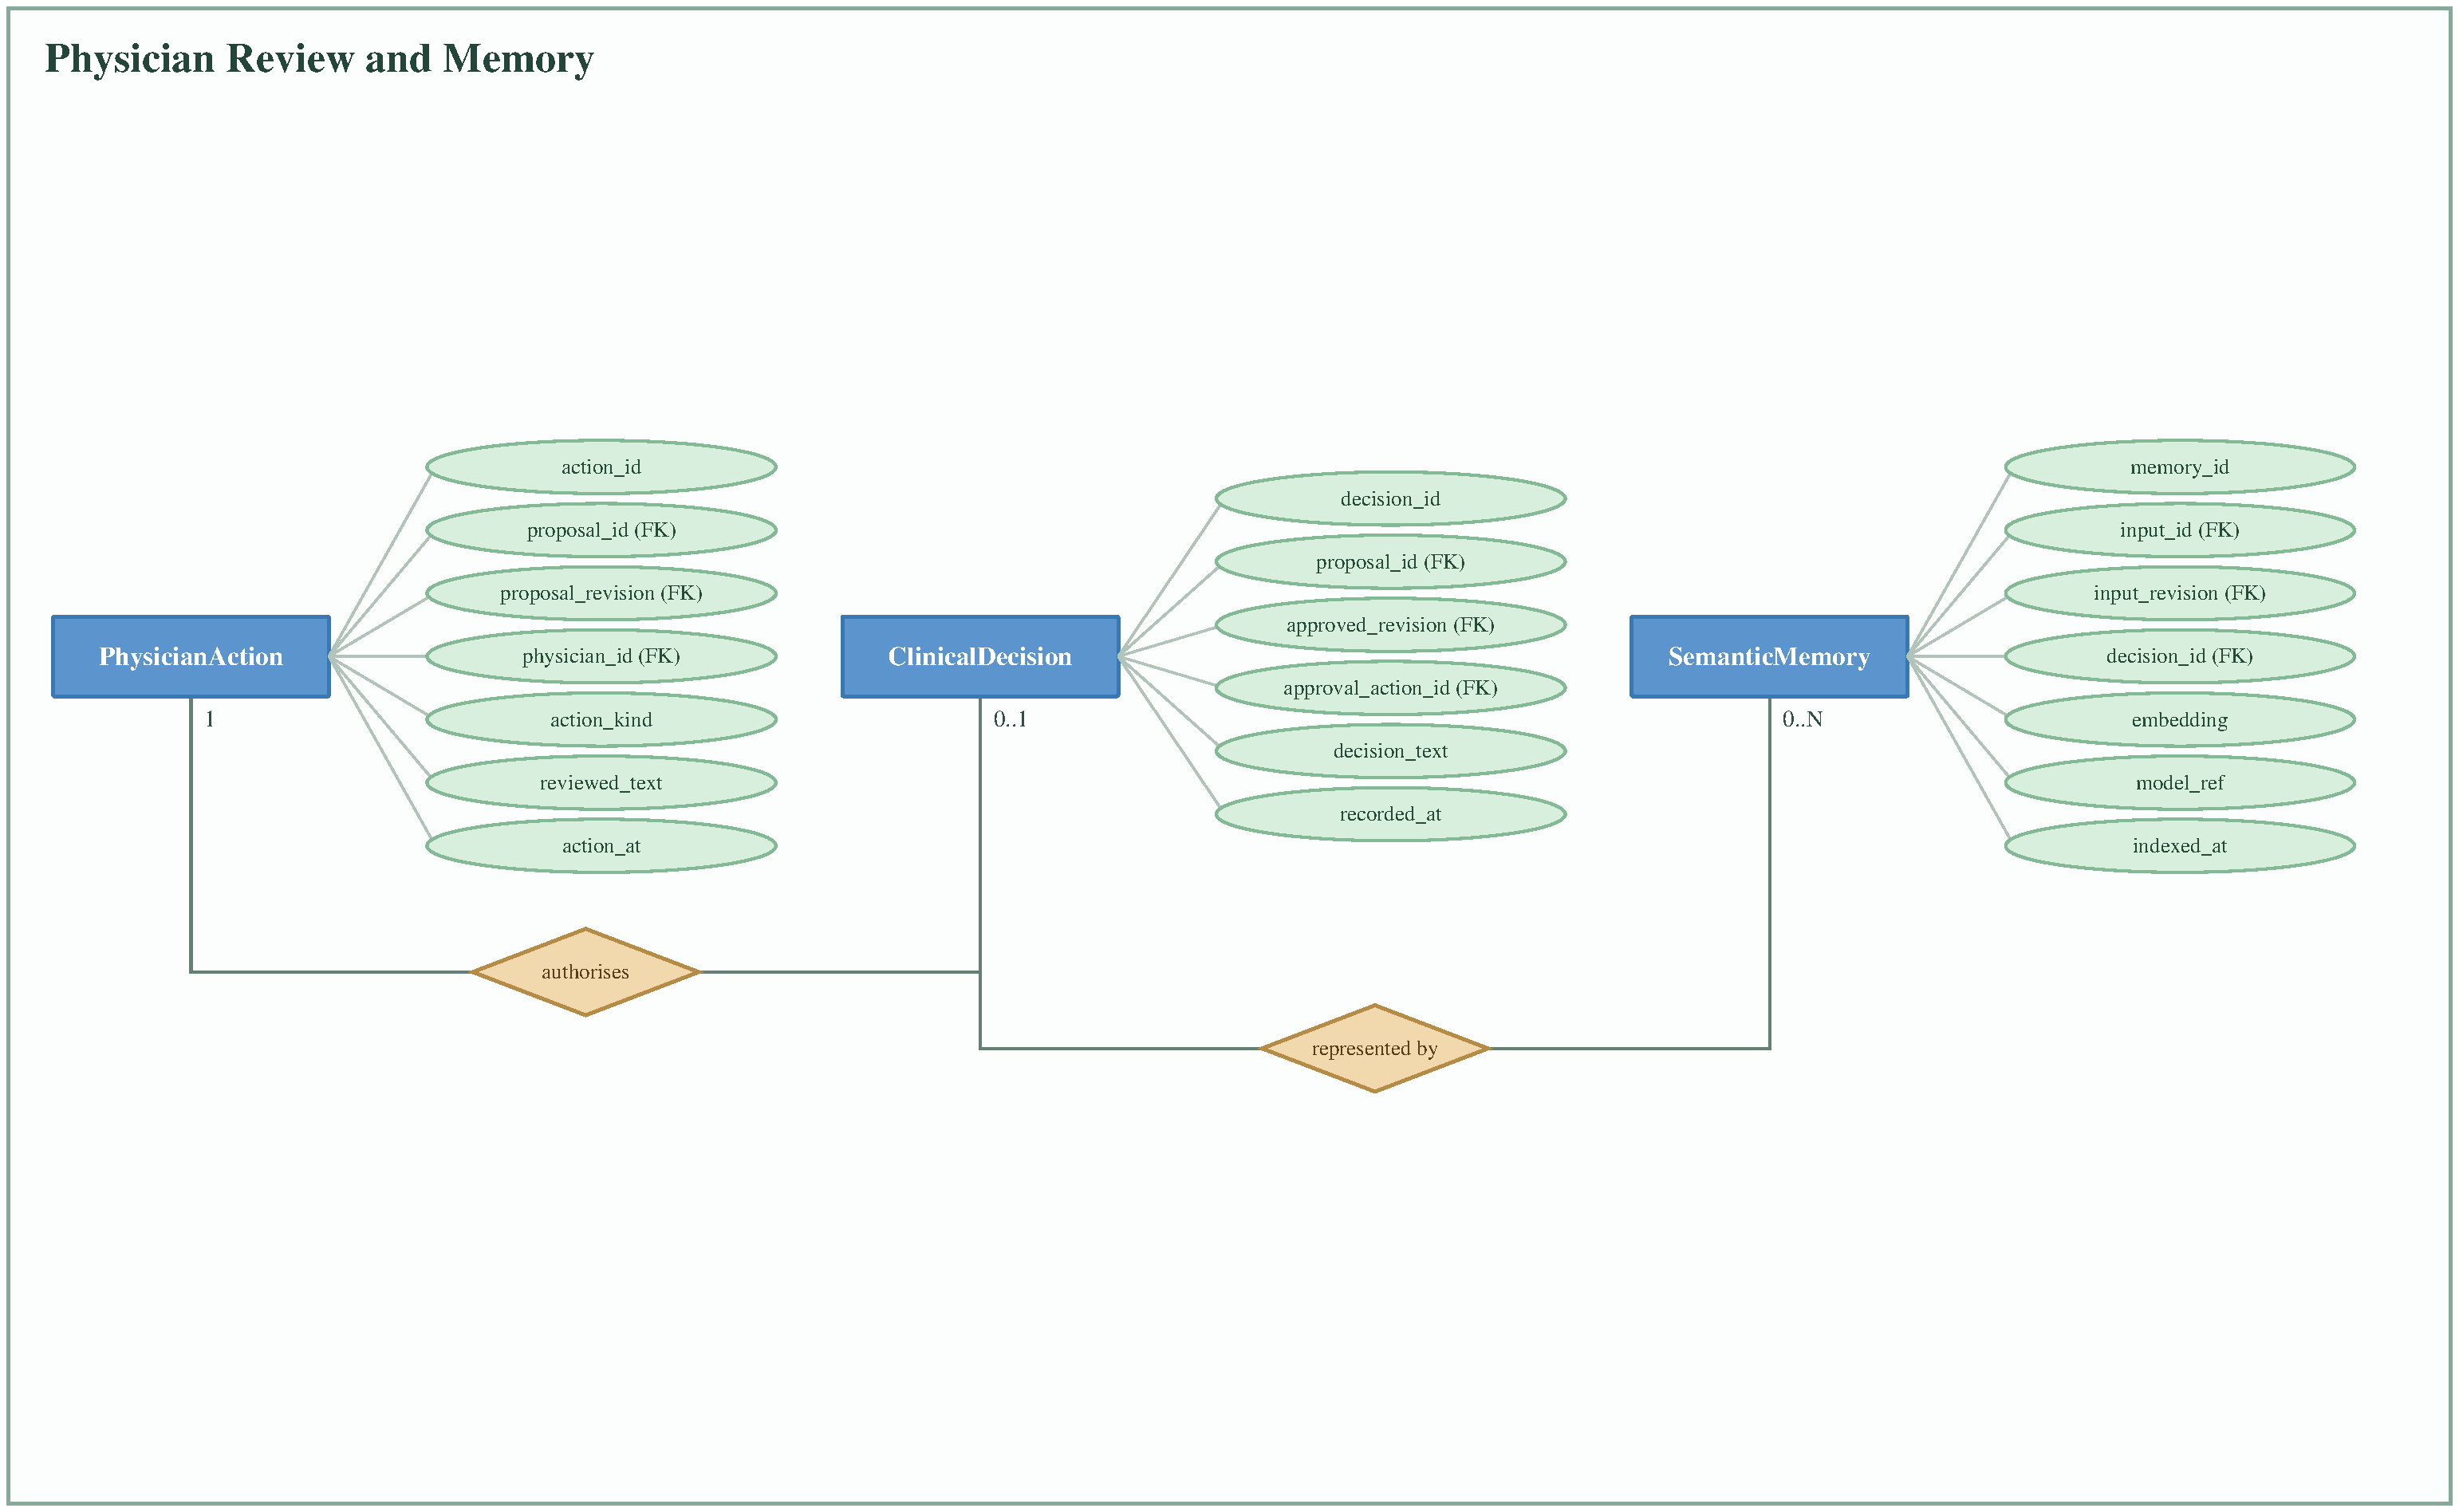
\includegraphics[width=\textwidth,height=0.80\textheight,keepaspectratio]{Figures/kashaf_D03_combined_review.pdf}
\caption{Physician actions, accepted decisions and semantic memory relationships.}
\label{fig:kashaf:er-review}
\end{figure}

\begin{figure}[!htbp]
\centering
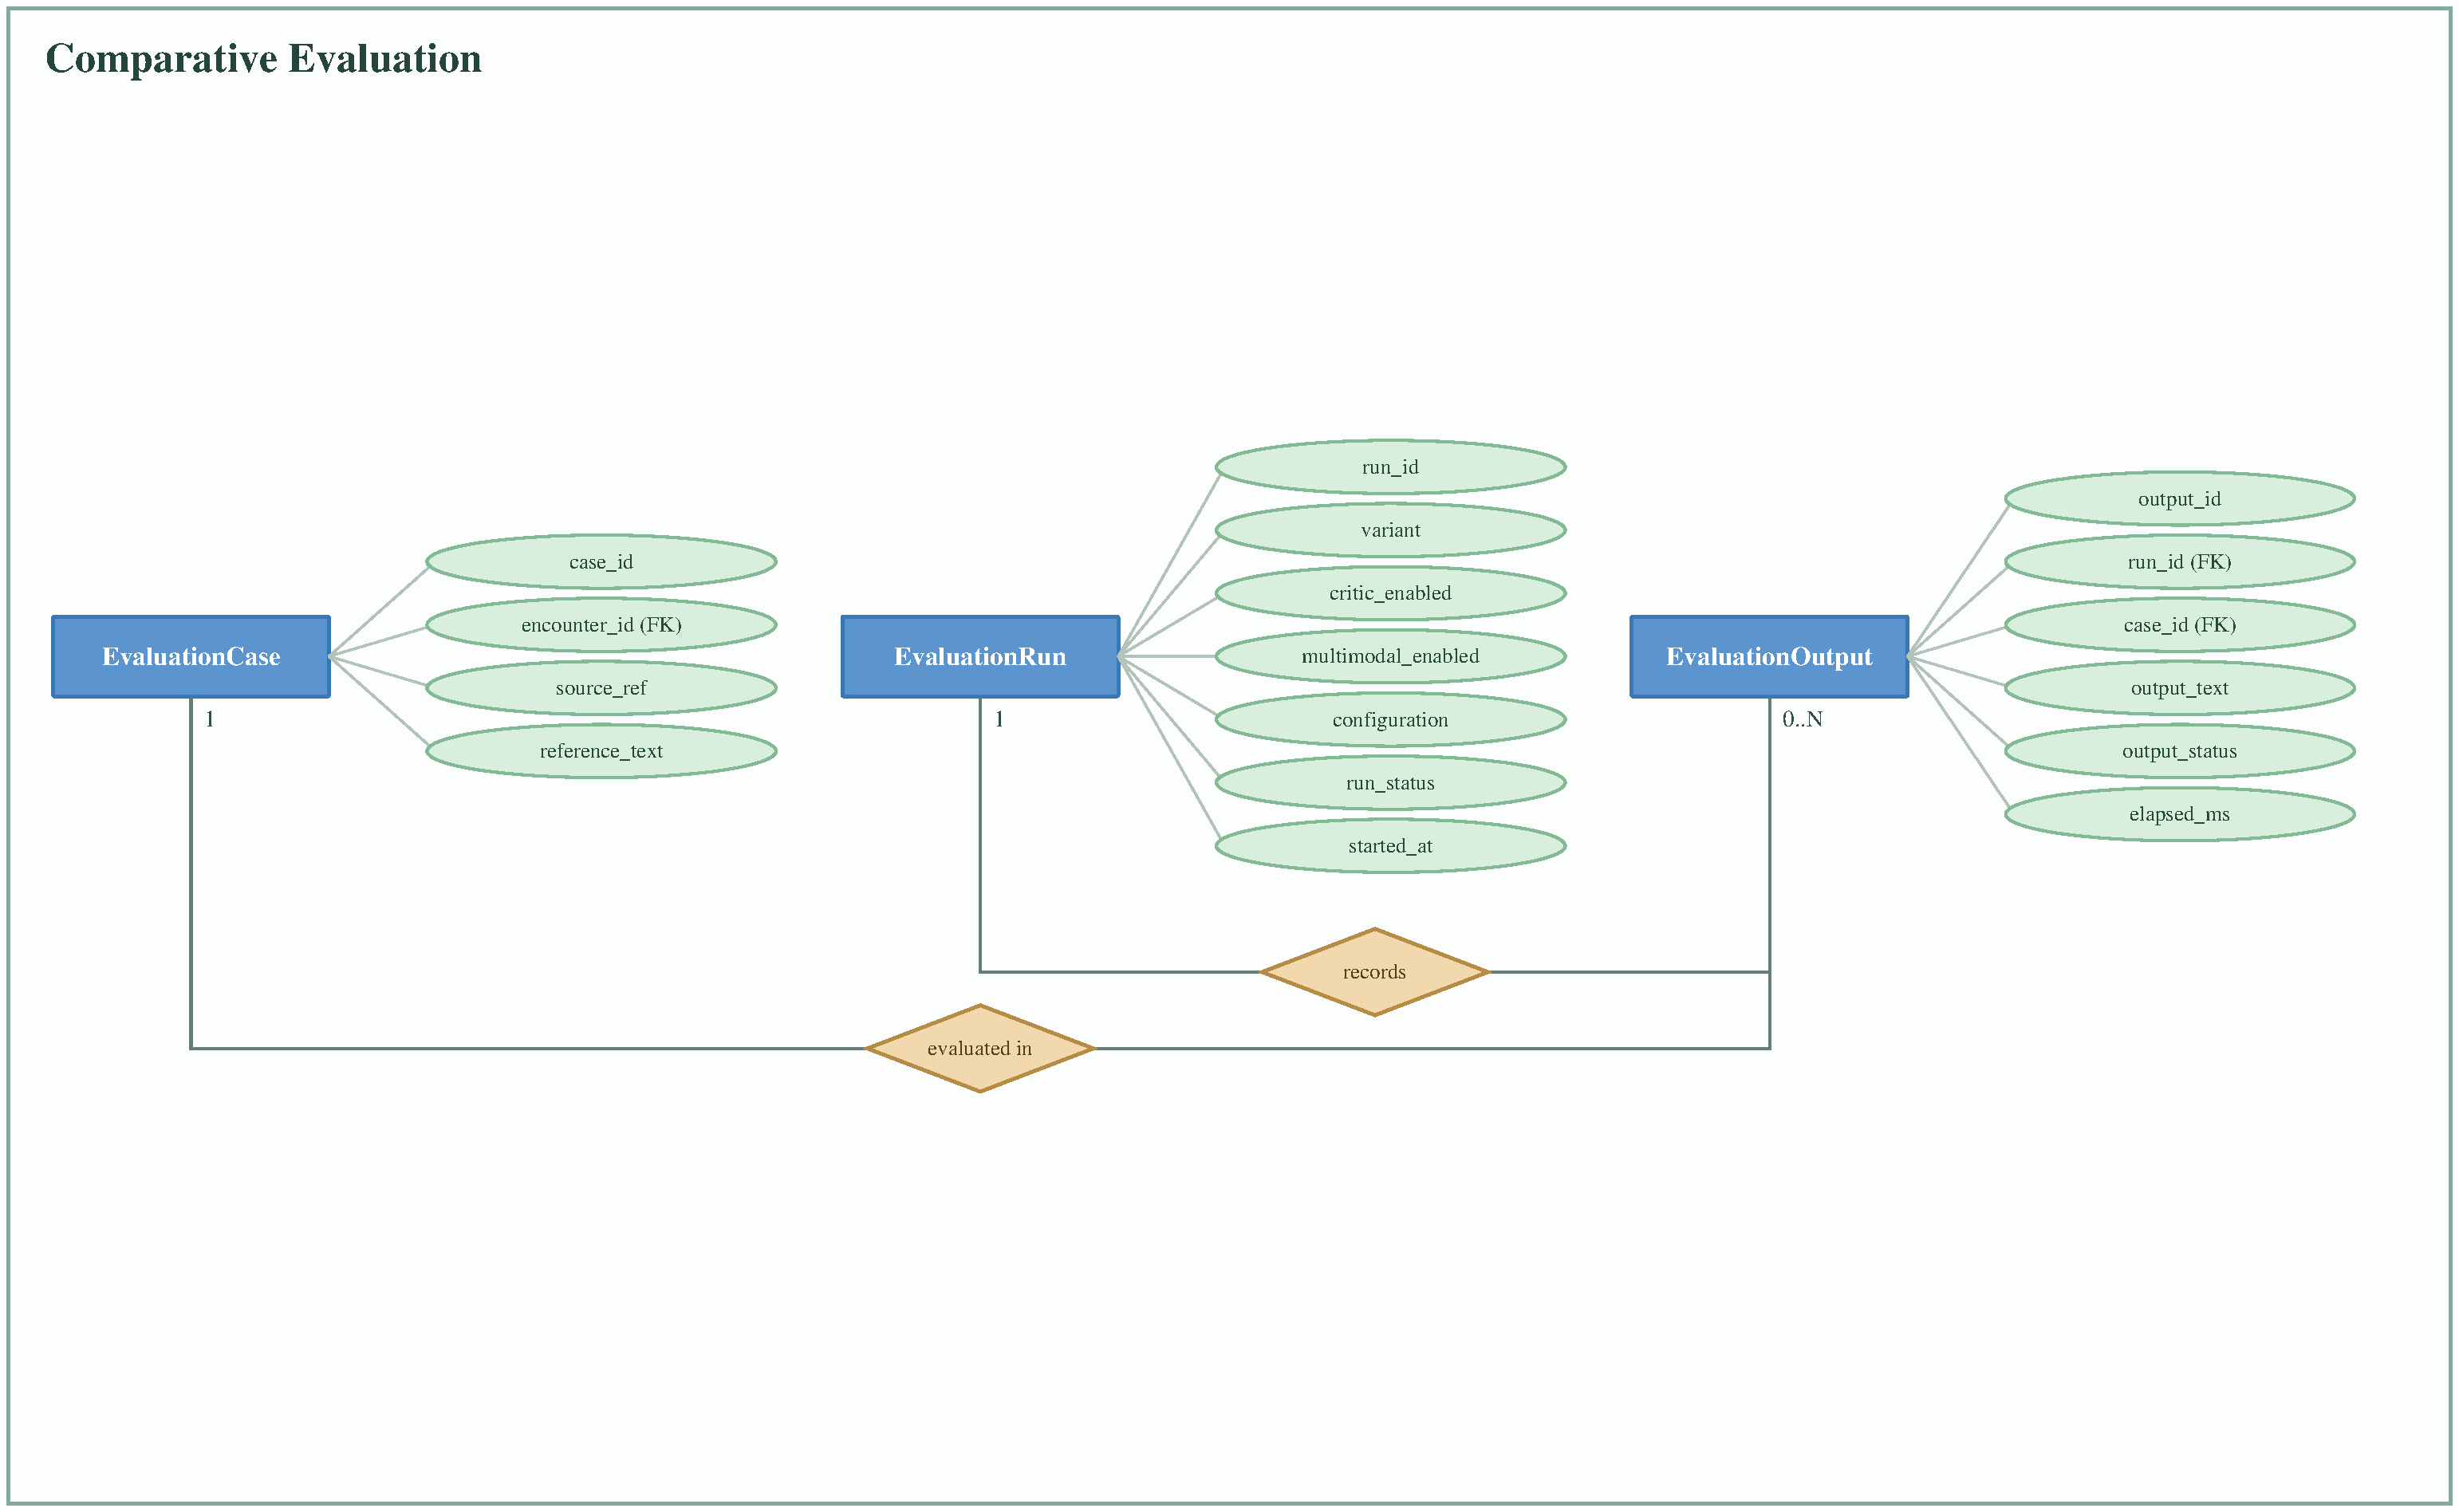
\includegraphics[width=\textwidth,height=0.80\textheight,keepaspectratio]{Figures/kashaf_D03_combined_evaluation.pdf}
\caption{Evaluation cases, configurations and recorded output relationships.}
\label{fig:kashaf:er-evaluation}
\end{figure}

\subsection{Data Dictionary}

Tables~\ref{tab:kashaf:dict-physician} onward define the entities, attributes, data types, constraints and meanings used by the logical schema. Primary keys identify records, composite keys preserve associations, and nullable fields accommodate absent values only where their processing state permits. Each patient's physician association governs access to encounters, case inputs, drafts, actions and decisions. Corrections create input revisions rather than replacing saved content; draft evidence, recorded critic findings and source links identify the exact revision they support. Approval validates the reviewed revision and physician action together, records matching accepted content, and permits at most one decision for that revision. Modified or rejected drafts remain outside accepted decisions. Semantic memory links authorised input revisions or approved decisions to their vector representations, with model-dependent dimensions configured after model selection. Evaluation fields describe case definitions, configurations and outputs; numerical measurements are populated only after an executed run. These relationships maintain source traceability without inventing missing clinical information.

\begin{reporttable}
\setlength{\tabcolsep}{5pt}
\centering
\small
\caption{Physician attributes, types and constraints.}
\label{tab:kashaf:dict-physician}
\begin{tabular}{|p{0.23\textwidth}|p{0.13\textwidth}|p{0.22\textwidth}|p{0.31\textwidth}|}
\hline
Attribute & Type & Constraints & Meaning \\ \hline
\texttt{physician\_id} & UUID & PK; not null & Unique physician account. \\ \hline
\texttt{full\_name} & text & Required; not null & Name supplied at registration. \\ \hline
\texttt{email} & text & Unique; not null & Normalised registration and login email. \\ \hline
\texttt{password\_hash} & text & Required; not null & Salted hash; plaintext passwords are never stored. \\ \hline
\texttt{created\_at} & timestamptz & Required; not null & Account creation time. \\ \hline
\end{tabular}
\end{reporttable}

\begin{reporttable}
\setlength{\tabcolsep}{5pt}
\centering
\small
\caption{Patient attributes, types and constraints.}
\label{tab:kashaf:dict-patient}
\begin{tabular}{|p{0.23\textwidth}|p{0.13\textwidth}|p{0.22\textwidth}|p{0.31\textwidth}|}
\hline
Attribute & Type & Constraints & Meaning \\ \hline
\texttt{patient\_id} & UUID & PK; not null & Unique patient record. \\ \hline
\texttt{physician\_id} & UUID & FK; not null & Physician who owns the record. \\ \hline
\texttt{patient\_ref} & text & Unique; not null & De-identified or synthetic reference. \\ \hline
\texttt{context\_text} & text & Optional; nullable & Available patient context. \\ \hline
\end{tabular}
\end{reporttable}

\begin{reporttable}
\setlength{\tabcolsep}{5pt}
\centering
\small
\caption{Encounter attributes, types and constraints.}
\label{tab:kashaf:dict-encounter}
\begin{tabular}{|p{0.23\textwidth}|p{0.13\textwidth}|p{0.22\textwidth}|p{0.31\textwidth}|}
\hline
Attribute & Type & Constraints & Meaning \\ \hline
\texttt{encounter\_id} & UUID & PK; not null & Unique encounter. \\ \hline
\texttt{patient\_id} & UUID & FK; not null & Patient associated with this encounter. \\ \hline
\texttt{recorded\_at} & timestamptz & Required; not null & Encounter date and time. \\ \hline
\end{tabular}
\end{reporttable}

\begin{reporttable}
\setlength{\tabcolsep}{5pt}
\centering
\small
\caption{ClinicalInput attributes, types and constraints.}
\label{tab:kashaf:dict-clinicalinput}
\begin{tabular}{|p{0.23\textwidth}|p{0.13\textwidth}|p{0.22\textwidth}|p{0.31\textwidth}|}
\hline
Attribute & Type & Constraints & Meaning \\ \hline
\texttt{input\_id} & UUID & PK; not null & Stable identifier of the supplied input. \\ \hline
\texttt{encounter\_id} & UUID & FK; not null & Encounter where the input originates. \\ \hline
\texttt{input\_kind} & text & Check; not null & Notes, imaging, laboratory or medication. \\ \hline
\end{tabular}
\end{reporttable}

\begin{reporttable}
\setlength{\tabcolsep}{5pt}
\centering
\small
\caption{InputRevision attributes, types and constraints.}
\label{tab:kashaf:dict-inputrevision}
\begin{tabular}{|p{0.23\textwidth}|p{0.13\textwidth}|p{0.22\textwidth}|p{0.31\textwidth}|}
\hline
Attribute & Type & Constraints & Meaning \\ \hline
\texttt{input\_id} & UUID & PK/FK; not null & Clinical input being versioned. \\ \hline
\texttt{revision\_no} & integer & PK; >0; not null & Saved revision of this input. \\ \hline
\texttt{content\_text} & text & Check; not null & Text content where applicable. \\ \hline
\texttt{file\_ref} & text & Check; not null & Stored file reference where applicable. \\ \hline
\texttt{recorded\_at} & timestamptz & Required; not null & Revision recording time. \\ \hline
\end{tabular}
\end{reporttable}

\begin{reporttable}
\setlength{\tabcolsep}{5pt}
\centering
\small
\caption{SpecialistFinding attributes, types and constraints.}
\label{tab:kashaf:dict-specialistfinding}
\begin{tabular}{|p{0.23\textwidth}|p{0.13\textwidth}|p{0.22\textwidth}|p{0.31\textwidth}|}
\hline
Attribute & Type & Constraints & Meaning \\ \hline
\texttt{finding\_id} & UUID & PK; not null & Unique analysis finding or processing record. \\ \hline
\texttt{input\_id} & UUID & FK pair; not null & Source clinical input. \\ \hline
\texttt{input\_revision} & integer & FK pair; not null & Exact analysed input revision. \\ \hline
\texttt{agent\_kind} & text & Check; not null & Imaging, laboratory or medication agent. \\ \hline
\texttt{model\_ref} & text & Optional; nullable & Model/resource identifier where applicable. \\ \hline
\texttt{finding\_text} & text & Check; not null & Available specialist findings. \\ \hline
\texttt{processing\_status} & text & Check; not null & Pending, complete or failed. \\ \hline
\texttt{processed\_at} & timestamptz & Optional; nullable & Completion or failure time. \\ \hline
\end{tabular}
\end{reporttable}

\begin{reporttable}
\setlength{\tabcolsep}{5pt}
\centering
\small
\caption{Proposal attributes, types and constraints.}
\label{tab:kashaf:dict-proposal}
\begin{tabular}{|p{0.23\textwidth}|p{0.13\textwidth}|p{0.22\textwidth}|p{0.31\textwidth}|}
\hline
Attribute & Type & Constraints & Meaning \\ \hline
\texttt{proposal\_id} & UUID & PK; not null & Stable identifier of a clinical draft. \\ \hline
\texttt{encounter\_id} & UUID & FK; not null & Encounter for which the draft is generated. \\ \hline
\texttt{created\_at} & timestamptz & Required; not null & Draft creation time. \\ \hline
\end{tabular}
\end{reporttable}

\begin{reporttable}
\setlength{\tabcolsep}{5pt}
\centering
\small
\caption{ProposalRevision attributes, types and constraints.}
\label{tab:kashaf:dict-proposalrevision}
\begin{tabular}{|p{0.23\textwidth}|p{0.13\textwidth}|p{0.22\textwidth}|p{0.31\textwidth}|}
\hline
Attribute & Type & Constraints & Meaning \\ \hline
\texttt{proposal\_id} & UUID & PK/FK; not null & Draft being versioned. \\ \hline
\texttt{revision\_no} & integer & PK; >0; not null & Saved draft revision. \\ \hline
\texttt{diagnosis\_text} & text & Required; not null & Generated or physician-edited diagnosis draft. \\ \hline
\texttt{treatment\_text} & text & Required; not null & Generated or physician-edited treatment draft. \\ \hline
\texttt{review\_status} & text & Check; not null & Pending, approved or rejected. \\ \hline
\texttt{created\_at} & timestamptz & Required; not null & Time this revision is saved. \\ \hline
\end{tabular}
\end{reporttable}

\begin{reporttable}
\setlength{\tabcolsep}{5pt}
\centering
\small
\caption{ProposalInput attributes, types and constraints.}
\label{tab:kashaf:dict-proposalinput}
\begin{tabular}{|p{0.23\textwidth}|p{0.13\textwidth}|p{0.22\textwidth}|p{0.31\textwidth}|}
\hline
Attribute & Type & Constraints & Meaning \\ \hline
\texttt{proposal\_id} & UUID & PK/FK pair; not null & Draft using the input. \\ \hline
\texttt{proposal\_revision} & integer & PK/FK pair; not null & Exact draft revision. \\ \hline
\texttt{input\_id} & UUID & PK/FK pair; not null & Current or historical source input. \\ \hline
\texttt{input\_revision} & integer & PK/FK pair; not null & Exact source input revision used. \\ \hline
\end{tabular}
\end{reporttable}

\begin{reporttable}
\setlength{\tabcolsep}{5pt}
\centering
\small
\caption{CriticReview attributes, types and constraints.}
\label{tab:kashaf:dict-criticreview}
\begin{tabular}{|p{0.23\textwidth}|p{0.13\textwidth}|p{0.22\textwidth}|p{0.31\textwidth}|}
\hline
Attribute & Type & Constraints & Meaning \\ \hline
\texttt{critic\_id} & UUID & PK; not null & Unique critic-review operation. \\ \hline
\texttt{proposal\_id} & UUID & FK pair; not null & Assessed clinical draft. \\ \hline
\texttt{proposal\_revision} & integer & FK pair; not null & Exact assessed revision. \\ \hline
\texttt{review\_status} & text & Check; not null & Pending, complete or failed. \\ \hline
\texttt{findings\_text} & text & Check; not null & Safety and consistency findings when complete. \\ \hline
\texttt{reviewed\_at} & timestamptz & Optional; nullable & Time the review completes or fails. \\ \hline
\end{tabular}
\end{reporttable}

\begin{reporttable}
\setlength{\tabcolsep}{5pt}
\centering
\small
\caption{EvidenceItem attributes, types and constraints.}
\label{tab:kashaf:dict-evidenceitem}
\begin{tabular}{|p{0.23\textwidth}|p{0.13\textwidth}|p{0.22\textwidth}|p{0.31\textwidth}|}
\hline
Attribute & Type & Constraints & Meaning \\ \hline
\texttt{evidence\_id} & UUID & PK; not null & Unique retrieved evidence item. \\ \hline
\texttt{source\_ref} & text & Required; not null & Citation or source reference. \\ \hline
\texttt{passage\_text} & text & Required; not null & Retrieved supporting passage. \\ \hline
\texttt{retrieved\_at} & timestamptz & Required; not null & Evidence retrieval time. \\ \hline
\end{tabular}
\end{reporttable}

\begin{reporttable}
\setlength{\tabcolsep}{5pt}
\centering
\small
\caption{ProposalEvidence attributes, types and constraints.}
\label{tab:kashaf:dict-proposalevidence}
\begin{tabular}{|p{0.23\textwidth}|p{0.13\textwidth}|p{0.22\textwidth}|p{0.31\textwidth}|}
\hline
Attribute & Type & Constraints & Meaning \\ \hline
\texttt{proposal\_id} & UUID & PK/FK pair; not null & Draft supported by evidence. \\ \hline
\texttt{proposal\_revision} & integer & PK/FK pair; not null & Exact supported revision. \\ \hline
\texttt{evidence\_id} & UUID & PK/FK; not null & Retrieved evidence item. \\ \hline
\end{tabular}
\end{reporttable}

\begin{reporttable}
\setlength{\tabcolsep}{5pt}
\centering
\small
\caption{PhysicianAction attributes, types and constraints.}
\label{tab:kashaf:dict-physicianaction}
\begin{tabular}{|p{0.23\textwidth}|p{0.13\textwidth}|p{0.22\textwidth}|p{0.31\textwidth}|}
\hline
Attribute & Type & Constraints & Meaning \\ \hline
\texttt{action\_id} & UUID & PK; not null & Unique physician review action. \\ \hline
\texttt{proposal\_id} & UUID & FK pair; not null & Clinical draft being reviewed. \\ \hline
\texttt{proposal\_revision} & integer & FK pair; not null & Exact reviewed revision. \\ \hline
\texttt{physician\_id} & UUID & FK; not null & Physician performing the action. \\ \hline
\texttt{action\_kind} & text & Check; not null & Modify, approve or reject. \\ \hline
\texttt{reviewed\_text} & text & Required; not null & Snapshot of the content associated with the action. \\ \hline
\texttt{action\_at} & timestamptz & Required; not null & Action recording time. \\ \hline
\end{tabular}
\end{reporttable}

\begin{reporttable}
\setlength{\tabcolsep}{5pt}
\centering
\small
\caption{ClinicalDecision attributes, types and constraints.}
\label{tab:kashaf:dict-clinicaldecision}
\begin{tabular}{|p{0.23\textwidth}|p{0.13\textwidth}|p{0.22\textwidth}|p{0.31\textwidth}|}
\hline
Attribute & Type & Constraints & Meaning \\ \hline
\texttt{decision\_id} & UUID & PK; not null & Unique approved clinical decision. \\ \hline
\texttt{proposal\_id} & UUID & FK pair; not null & Originating clinical draft. \\ \hline
\texttt{approved\_revision} & integer & FK pair; unique pair; not null & Explicitly accepted draft revision. \\ \hline
\texttt{approval\_action\_id} & UUID & Unique FK; not null & Matching physician approval action. \\ \hline
\texttt{decision\_text} & text & Required; not null & Exact accepted diagnosis and treatment content. \\ \hline
\texttt{recorded\_at} & timestamptz & Required; not null & Decision recording time. \\ \hline
\end{tabular}
\end{reporttable}

\begin{reporttable}
\setlength{\tabcolsep}{5pt}
\centering
\small
\caption{SemanticMemory attributes, types and constraints.}
\label{tab:kashaf:dict-semanticmemory}
\begin{tabular}{|p{0.23\textwidth}|p{0.13\textwidth}|p{0.22\textwidth}|p{0.31\textwidth}|}
\hline
Attribute & Type & Constraints & Meaning \\ \hline
\texttt{memory\_id} & UUID & PK; not null & Unique semantic representation. \\ \hline
\texttt{input\_id} & UUID & FK pair; not null & Input source when applicable. \\ \hline
\texttt{input\_revision} & integer & FK pair; not null & Exact input-source revision. \\ \hline
\texttt{decision\_id} & UUID & FK; not null & Approved-decision source when applicable. \\ \hline
\texttt{embedding} & vector(TBD) & Required; not null & Vector using the selected embedding dimension. \\ \hline
\texttt{model\_ref} & text & Required; not null & Embedding model identifier and version. \\ \hline
\texttt{indexed\_at} & timestamptz & Required; not null & Indexing time. \\ \hline
\end{tabular}
\end{reporttable}

\begin{reporttable}
\setlength{\tabcolsep}{5pt}
\centering
\small
\caption{EvaluationCase attributes, types and constraints.}
\label{tab:kashaf:dict-evaluationcase}
\begin{tabular}{|p{0.23\textwidth}|p{0.13\textwidth}|p{0.22\textwidth}|p{0.31\textwidth}|}
\hline
Attribute & Type & Constraints & Meaning \\ \hline
\texttt{case\_id} & UUID & PK; not null & Unique permitted evaluation case. \\ \hline
\texttt{encounter\_id} & UUID & FK; not null & Case encounter supplying clinical context. \\ \hline
\texttt{source\_ref} & text & Required; not null & Dataset or synthetic-case provenance. \\ \hline
\texttt{reference\_text} & text & Optional; nullable & Reference assessment when established. \\ \hline
\end{tabular}
\end{reporttable}

\begin{reporttable}
\setlength{\tabcolsep}{5pt}
\centering
\small
\caption{EvaluationRun attributes, types and constraints.}
\label{tab:kashaf:dict-evaluationrun}
\begin{tabular}{|p{0.23\textwidth}|p{0.13\textwidth}|p{0.22\textwidth}|p{0.31\textwidth}|}
\hline
Attribute & Type & Constraints & Meaning \\ \hline
\texttt{run\_id} & UUID & PK; not null & Unique configured research run. \\ \hline
\texttt{variant} & text & Check; not null & Single LLM, memory-augmented or full Zeest. \\ \hline
\texttt{critic\_enabled} & boolean & Required; not null & Declared critic configuration. \\ \hline
\texttt{multimodal\_enabled} & boolean & Required; not null & Declared multimodal configuration. \\ \hline
\texttt{configuration} & jsonb & Required; not null & Model/resource versions and comparison settings. \\ \hline
\texttt{run\_status} & text & Check; not null & Configured, running, complete or failed. \\ \hline
\texttt{started\_at} & timestamptz & Optional; nullable & Actual run start time, when executed. \\ \hline
\end{tabular}
\end{reporttable}

\begin{reporttable}
\setlength{\tabcolsep}{5pt}
\centering
\small
\caption{EvaluationOutput attributes, types and constraints.}
\label{tab:kashaf:dict-evaluationoutput}
\begin{tabular}{|p{0.23\textwidth}|p{0.13\textwidth}|p{0.22\textwidth}|p{0.31\textwidth}|}
\hline
Attribute & Type & Constraints & Meaning \\ \hline
\texttt{output\_id} & UUID & PK; not null & Unique run/case output. \\ \hline
\texttt{run\_id} & UUID & FK; unique pair; not null & Research run producing this output. \\ \hline
\texttt{case\_id} & UUID & FK; unique pair; not null & Evaluation case used by the run. \\ \hline
\texttt{output\_text} & text & Check; not null & Recorded system output after execution. \\ \hline
\texttt{output\_status} & text & Check; not null & Pending, complete or failed. \\ \hline
\texttt{elapsed\_ms} & numeric & Optional; >=0; nullable & Measured duration only when available. \\ \hline
\end{tabular}
\end{reporttable}


\section{ Risk Analysis}

\begin{reporttable}
\centering
\small
\caption{Project risks, consequences and intended responses.}
\label{tab:kashaf:risks}
\begin{tabular}{|p{0.06\textwidth}|p{0.2\textwidth}|p{0.27\textwidth}|p{0.33\textwidth}|}
\hline
ID & Risk & Consequence & Response \\ \hline
R01 & Data/model access & The selected clinical domain cannot be supported. & Confirm permitted cases and validated models before integration. \\ \hline
R02 & Transcription/input quality & Incomplete or incorrect case information. & Allow note correction and report unusable inputs. \\ \hline
R03 & Insufficient evidence & Draft recommendations lack inspectable support. & Show retrieved sources and make missing evidence explicit. \\ \hline
R04 & Unsupported reasoning & Recommendations contain inconsistent findings. & Use critic review and retain physician decision authority. \\ \hline
R05 & Patient-context mismatch & History or inputs are assigned to the wrong case. & Validate patient/encounter keys across processing and storage. \\ \hline
R06 & Approval/revision error & Recorded content differs from the physician-approved draft. & Bind approval to the exact revision and content snapshot. \\ \hline
R07 & Integration/service failure & The processing workflow is incomplete or incompatible. & Define contracts and expose stage-specific failures. \\ \hline
R08 & Evaluation resources & Variant comparisons cannot answer the research questions. & Agree references, common cases and comparison conditions. \\ \hline
\end{tabular}
\end{reporttable}

% Finish this section's floats before the next heading.

Table~\ref{tab:kashaf:risks} outlines risks concerning resource permissions, supported clinical coverage, incomplete evidence, incorrect patient context and revision-specific approval. Their responses establish verification activities rather than completed mitigation outcomes. Dataset and model selection must confirm permitted use and task suitability before cases enter processing or comparison. Source identifiers and ownership checks must remain consistent through retrieval, analysis and review, while unavailable resources require visible failure states. Evidence inspection and critic findings support physician judgement without guaranteeing correctness. Approval must accept the reviewed revision and preserve matching action and decision records, including when requests fail or repeat. Integration tests and controlled comparisons are needed to assess these responses after implementation. The requirements, use cases, interface designs and logical schema therefore define a clinical workflow, while the methodology and architecture specify how its behaviour can be investigated. No performance result, executed acceptance test or demonstrated clinical safety outcome is established by these design artefacts.

\section{Conclusion}

The requirements establish a connected workflow from account access and physician-specific patient selection to consultation capture, specialist findings and clinical review. Functional requirements identify the operations users need, while quality attributes and non-functional requirements define ownership, integrity, traceability and understandable processing states. Use-case tables describe normal and alternative paths, and interface mappings connect these interactions to the corresponding screens. The logical schema preserves input revisions, draft sources, review actions and accepted decisions so corrections and approval refer to identifiable content. Registration supports account access without introducing additional clinical roles, and each physician remains restricted to their own patients. Together, these specifications make the intended behaviour assessable through functional and integrity checks. Numerical performance limits and clinical resource configurations require an agreed environment before measurement. The requirements provide the contract for implementation and evaluation; they do not establish completed acceptance tests or clinical effectiveness. Subsequent design must preserve these relationships when connecting application services, agents and storage.

\endgroup
